%%%%%%%%%%%%%%%%%%%%%%%%%%%%%%%%%%%%%%%%%%%%%%%%%%%%%%%%%%%%%%%%%%%%%%
% Overleaf (WriteLaTeX) Example: Molecular Chemistry Presentation
%
% Source: http://www.overleaf.com
%
% In these slides we show how Overleaf can be used with standard 
% chemistry packages to easily create professional presentations.
% 
% Feel free to distribute this example, but please keep the referral
% to overleaf.com
% 
%%%%%%%%%%%%%%%%%%%%%%%%%%%%%%%%%%%%%%%%%%%%%%%%%%%%%%%%%%%%%%%%%%%%%%
% How to use Overleaf: 
%
% You edit the source code here on the left, and the preview on the
% right shows you the result within a few seconds.
%
% Bookmark this page and share the URL with your co-authors. They can
% edit at the same time!
%
% You can upload figures, bibliographies, custom classes and
% styles using the files menu.
%
% If you're new to LaTeX, the wikibook is a great place to start:
% http://en.wikibooks.org/wiki/LaTeX
%
%%%%%%%%%%%%%%%%%%%%%%%%%%%%%%%%%%%%%%%%%%%%%%%%%%%%%%%%%%%%%%%%%%%%%%

\documentclass[hyperref={colorlinks,citecolor=blue,linkcolor=blue,urlcolor=blue}]{beamer}

% For more themes, color themes and font themes, see:
% http://deic.uab.es/~iblanes/beamer_gallery/index_by_theme.html
%
\mode<presentation>
{
  \usetheme{Madrid}       % or try default, Darmstadt, Warsaw, ...
  \usecolortheme{default} % or try albatross, beaver, crane, ...
  \usefonttheme{serif}    % or try default, structurebold, ...
  \setbeamertemplate{navigation symbols}{}
  \setbeamertemplate{caption}[numbered]
} 

\usepackage[english]{babel}
\usepackage[utf8x]{inputenc}
\usepackage{chemfig}
\usepackage[version=3]{mhchem}
\usepackage{tikz}
\usetikzlibrary{plotmarks}
\usepackage{pgfplots}
\usepackage{lineno}
\usepackage{tikz}
\usepackage{xcolor}
\usepackage{subcaption}
\usepackage{pgf}  
\usepackage{svg}
\usepackage{ragged2e}
\usepackage{booktabs}
\usepackage{float}
\usepackage{caption}
\captionsetup{font=footnotesize}
\usepackage{xcolor}
\usepackage{nccmath} 
% \usetikzlibrary{external}
% \tikzexternalize[prefix=figures/generated/]
\newlength\figureheight
\newlength\figurewidth
% \addtobeamertemplate{navigation symbols}{}{%
%     \usebeamerfont{footline}%
%     \usebeamercolor[fg]{footline}%
%     \hspace{5em}%
%     \insertframenumber/\inserttotalframenumber
% }
% Syntax: \colorboxed[<color model>]{<color specification>}{<math formula>}
\newcommand*{\colorboxed}{}
\def\colorboxed#1#{%
  \colorboxedAux{#1}%
}
\newcommand*{\colorboxedAux}[3]{%
  % #1: optional argument for color model
  % #2: color specification
  % #3: formula
  \begingroup
    \colorlet{cb@saved}{.}%
    \color#1{#2}%
    \boxed{%
      \color{cb@saved}%
      #3%
    }%
  \endgroup
}
\setbeamertemplate{navigation symbols}{}
% \setbeamertemplate{footline}[frame number]{}
\setbeamertemplate{page number in head/foot}[totalframenumber]


\setbeamertemplate{footline}
{
  \leavevmode%
  \hbox{%
    \begin{beamercolorbox}[wd=0.33\paperwidth,ht=2.5ex,dp=1.125ex,left]{author in head/foot}%
      \tiny \hspace{1em}Cristian A. Blanco Martínez
    \end{beamercolorbox}%
    \begin{beamercolorbox}[wd=0.34\paperwidth,ht=2.5ex,dp=1.125ex,center]{institute in head/foot}%
      \tiny Universidad Tecnológica de Pereira
    \end{beamercolorbox}%
    \begin{beamercolorbox}[wd=0.33\paperwidth,ht=2.5ex,dp=1.125ex,right]{date in head/foot}%
      \tiny {\tiny \insertshortdate{}} \hspace{1em} {\tiny \insertframenumber{} / \inserttotalframenumber} \hspace{1em}
    \end{beamercolorbox}%
  }%
  \vskip0pt%
}



% On Overleaf, these lines give you sharper preview images.
% You might want to `comment them out before you export, though.
\usepackage{pgfpages}
\pgfpagesuselayout{resize to}[%
  physical paper width=8in, physical paper height=6in]

% Here's where the presentation starts, with the info for the title slide
\title[]{Optimization and Prediction in Natural Gas Networks Using Graph Neural Networks and MPCC-Based Models}
% \author{Cristian Alejandro Blanco Martínez}
\author{
    \texorpdfstring{
        \begin{tabular}{c}
            Author: Cristian Alejandro Blanco Martínez \\
            Director: David Augusto Cárdenas Peña
        \end{tabular}
    }{Cristian Alejandro Blanco Martínez, David Augusto Cárdenas Peña}
}

\institute{Universidad Tecnológica de Pereira \\ 
Grupo de investigación Automática}
\date{\scriptsize \today}

\begin{document}

\begin{frame}
  \titlepage

  \vfill % Empuja los logos hacia la parte inferior
  \begin{minipage}{0.32\linewidth}
    
\includegraphics[height=2cm]{figures/logos/utp.jpg}
  \end{minipage}
  \hfill
  \begin{minipage}{0.32\linewidth}
    \flushright
    
\includegraphics[height=2cm]{figures/logos/mie.jpg}
  \end{minipage}
  \hfill
  \begin{minipage}{0.32\linewidth}
    \centering
    
\includegraphics[height=2cm]{figures/logos/automatica.jpeg}
  \end{minipage}
\end{frame}

\begin{frame}{Agenda}
  \tableofcontents
\end{frame}


\section{Motivation \& Problem Statement}
\begin{frame}{Energy Context \& Relevance of Natural Gas}
\footnotesize
\justifying
In Colombia, natural gas is widely used across the residential, commercial, industrial, and thermal power sectors. Its importance becomes evident during dry seasons, when hydroelectric generation is reduced and thermal plants, fueled by natural gas, step in to maintain electricity supply  \cite{Promigas_2021}.
\\
\begin{figure}[h]
    \centering
    \footnotesize
    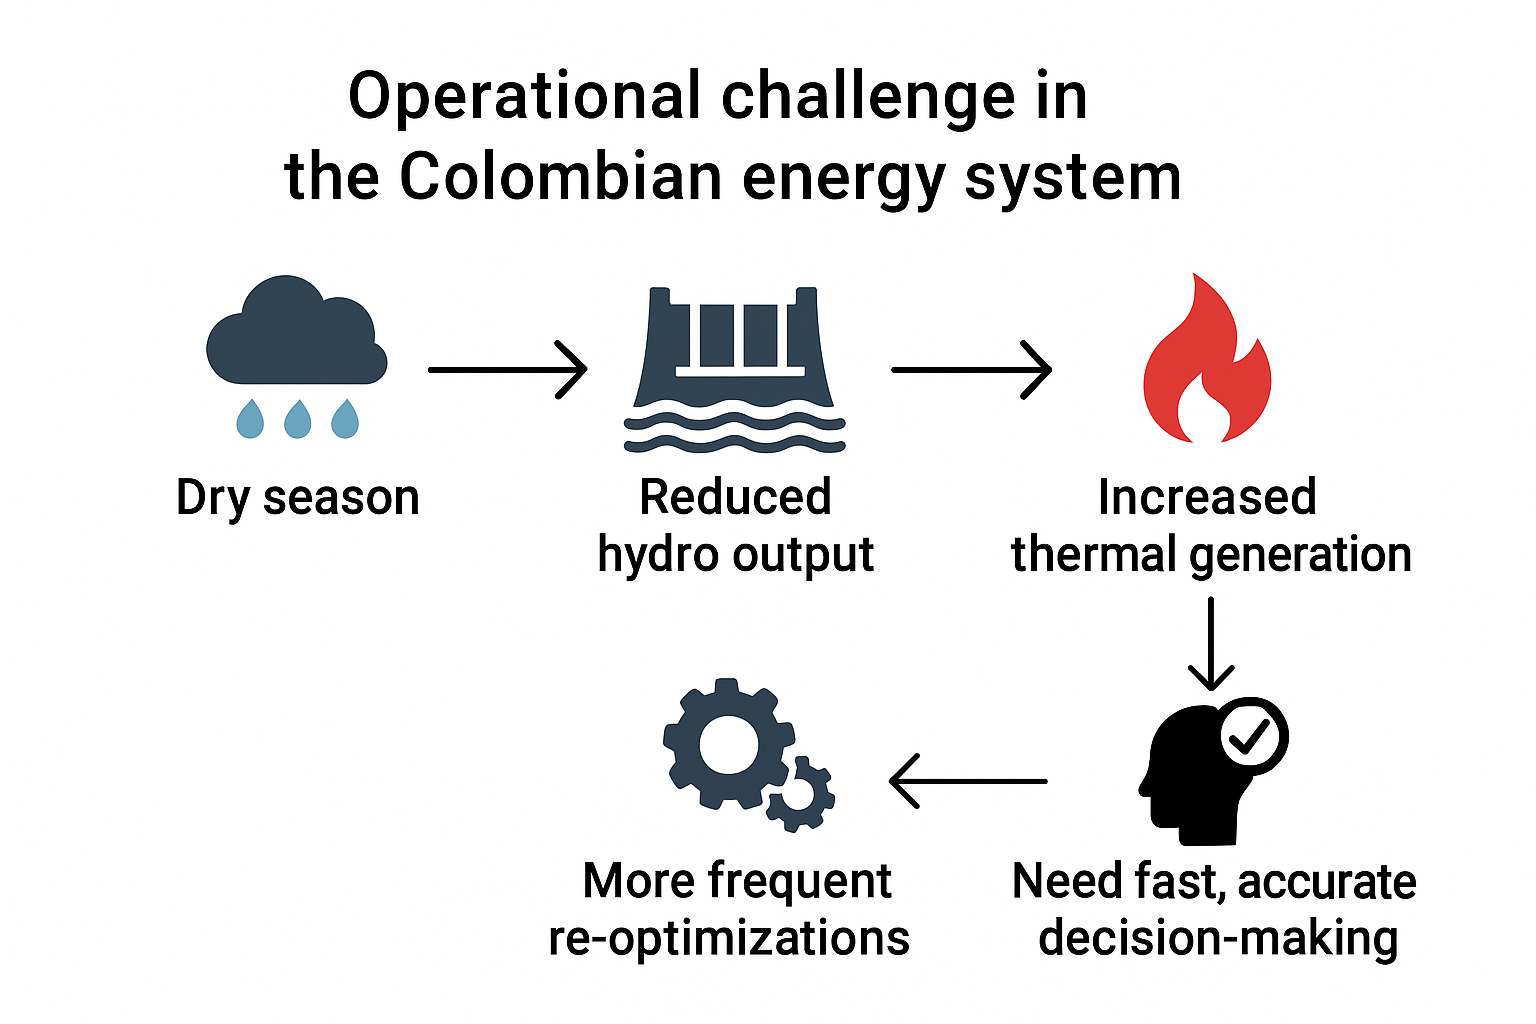
\includegraphics[width=0.6\textwidth]{figures/hydro_vs_thermal.png}
\end{figure}
\end{frame}


\begin{frame}{Motivation \& Problem Statement}
\justifying
\footnotesize 

\begin{itemize}
    \footnotesize 
    \item \textbf{Large-scale natural gas networks} require solving complex optimization problems \cite{9831787}.
    \item Increasing network size and operational constraints lead to:
    \begin{itemize}
        \footnotesize 
        \item Long execution times
        \item Difficulty in real-time or near real-time decision making
    \end{itemize}
    \item Classical approaches are accurate but often \textbf{computationally expensive}.
\end{itemize}

\textit{Solving a network with 592 nodes and 460 edges takes ~5 min on average, while a larger one with 660 nodes and more than 500 edges requires ~30 min using the same MILP-based optimizer \cite{artice_time_comparison}}.

\vspace{0.5cm}
\textbf{Main Problem:} There is a need for methods that preserve accuracy while significantly reducing computation time.
\end{frame}



\begin{frame}{Problem Statement: Specific Challenges}
\justifying
\footnotesize
From the general problem of natural gas transportation optimization, three specific challenges can be identified:
\begin{enumerate}
    \footnotesize
    \item \textbf{High computational cost:}  
    Solving large-scale optimization problems requires long execution times, limiting the feasibility of real-time or near real-time operation.

    \item \textbf{Pipeline modeling complexity:}  
    The Weymouth equation introduces nonlinearities, discontinuities, and nonconvexities that generate approximation errors and numerical instability.

    \item \textbf{Uncertainty in demand:}  
    Variability in hydropower generation and the growth of renewable sources create uncertainty in the demand for natural gas, requiring flexible and stochastic optimization approaches.
\end{enumerate}

\vspace{0.5cm}
\textbf{Research Question:} How can an optimization tool be developed that seeks to improve the solution to the problem of natural gas transportation, taking into account computational cost, growing energy demand, and the uncertainty associated with this factor?
\end{frame}



\section{Objectives}
\begin{frame}{Objectives}
\footnotesize
\textbf{General Objective:}
\begin{itemize}
    \item Develop an optimization tool that integrates knowledge of the gas transportation network topology, a suitable approximation of the Weymouth equation and stochastic optimization techniques to address the gas transportation task taking into account the uncertainties related to hydroelectric generation and the growth of alternative energy sources.
\end{itemize}

    \textbf{Specific Objectives:}
\begin{enumerate}
    \footnotesize
    \item Design a Graph Neural Networks-based approach of regression that integrates knowledge of natural gas network topology to reduce computational time for operation estimation.    
    \item Develop an optimization model for natural gas transportation systems that takes into account the Weymouth equation for reducing that reduces the approximation error in pipeline gas flow calculations.
    \item Develop a stochastic gas flow dispatch optimization strategy that quantifies the uncertainty in the objective variables and decision variables associated with the operation of the gas system taking into account the constraints of the transportation problem.
\end{enumerate}
\end{frame}


\section{Objective 1 - Natural Gas System Prediction Using Graph Neural Networks}
\begin{frame}{Objective 1 - Natural Gas System as a Graph}
    \footnotesize
    \justifying
    A natural gas network can be represented as a directed graph, 
    where nodes correspond to elements such as wells, users, or storage facilities, 
    and edges represent pipelines and compressors.
    
    % Dividimos el slide en dos columnas usando minipage
    \begin{minipage}[c]{0.48\linewidth}
        \centering
        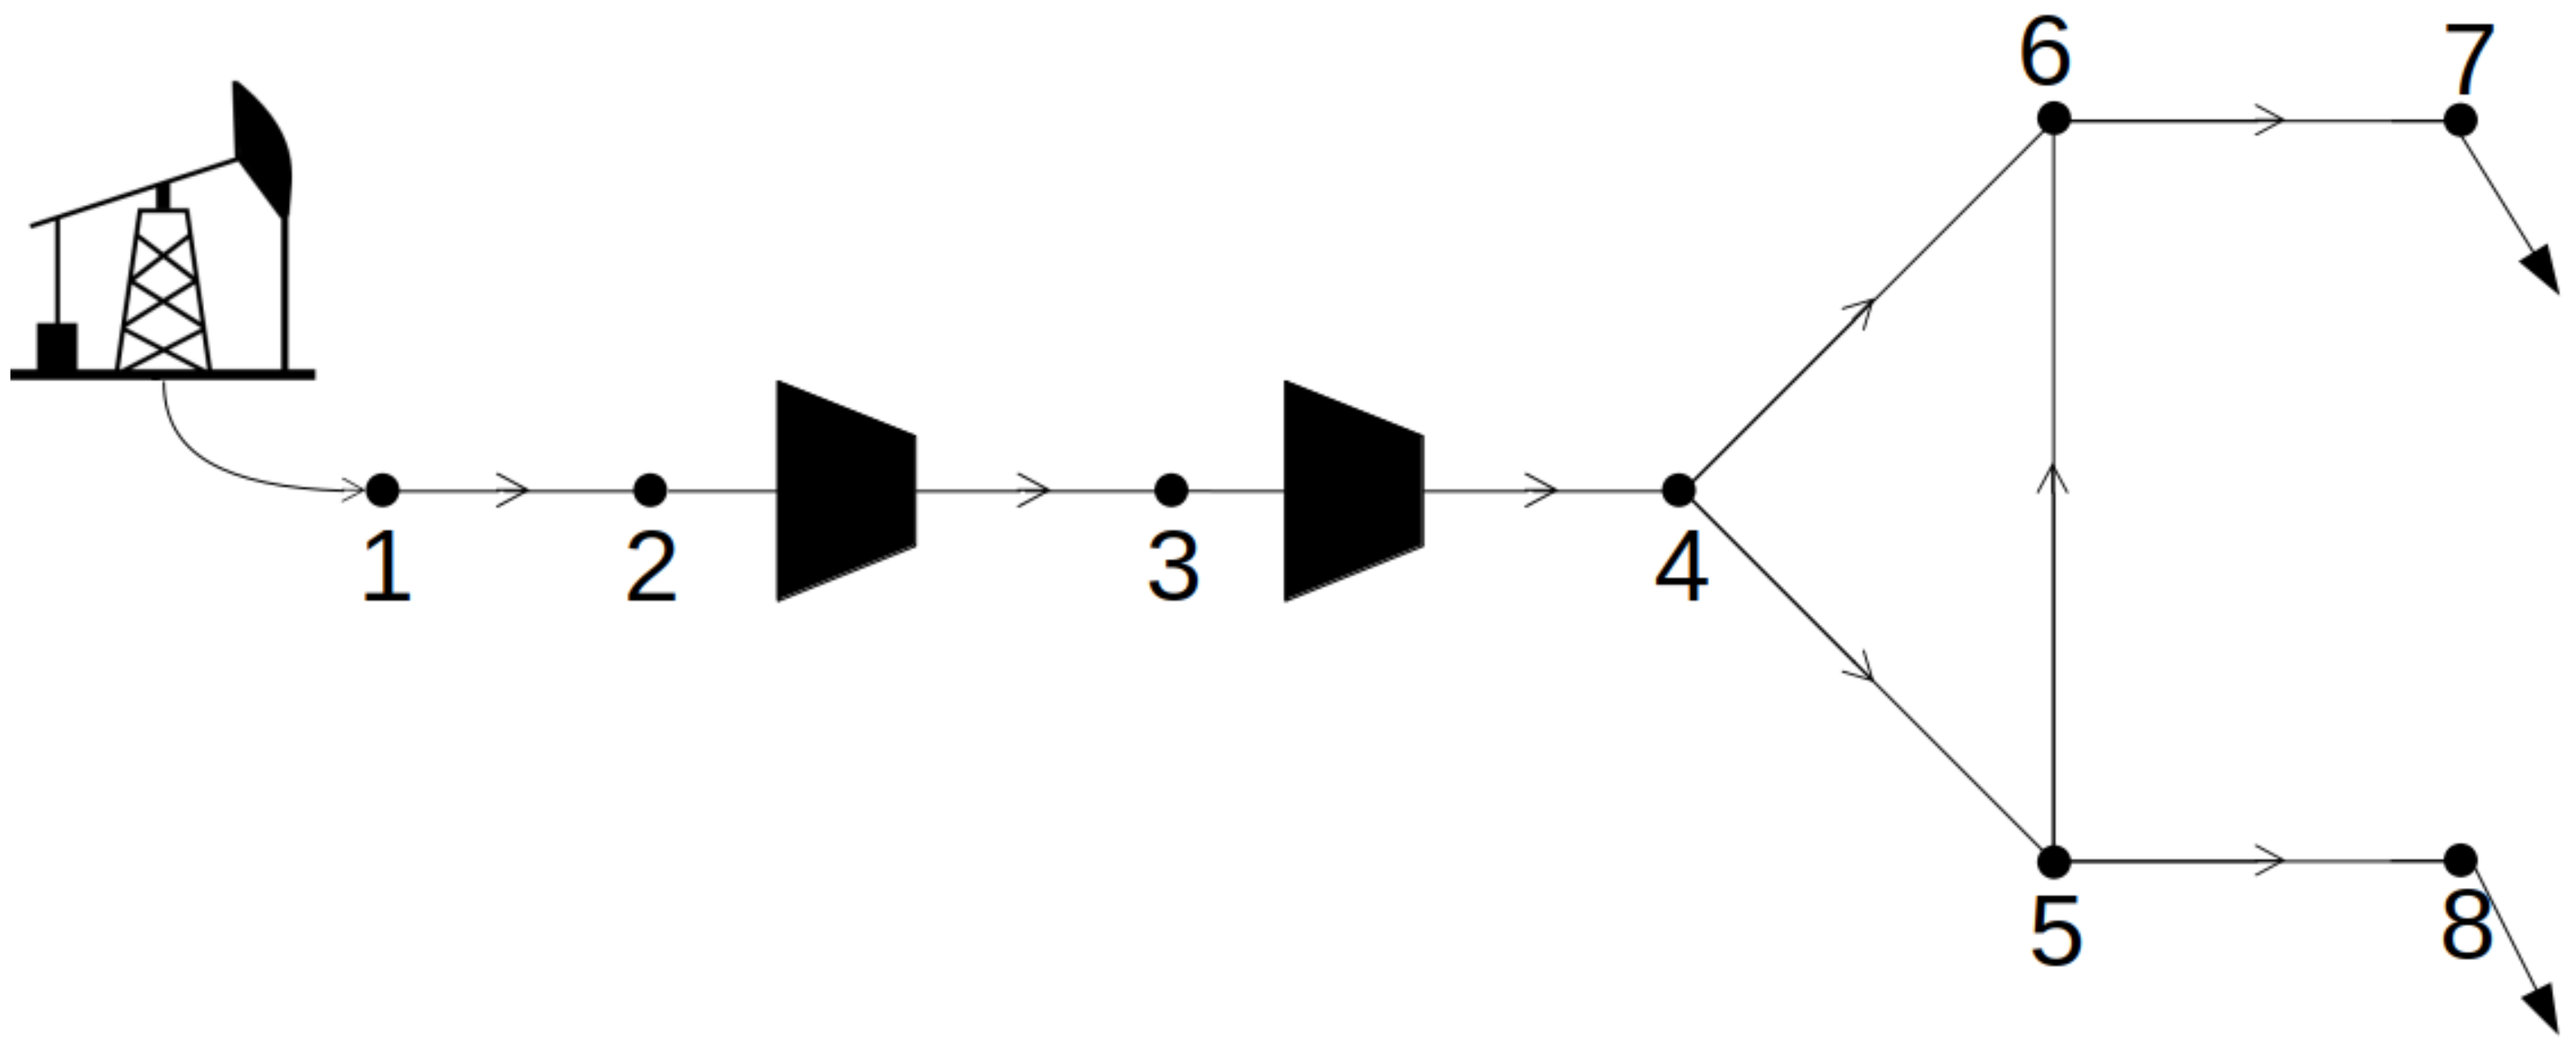
\includegraphics[width=1\linewidth]{figures/8_node_system.png} 
    \end{minipage}\hfill
    \begin{minipage}[c]{0.48\linewidth}
        \centering
        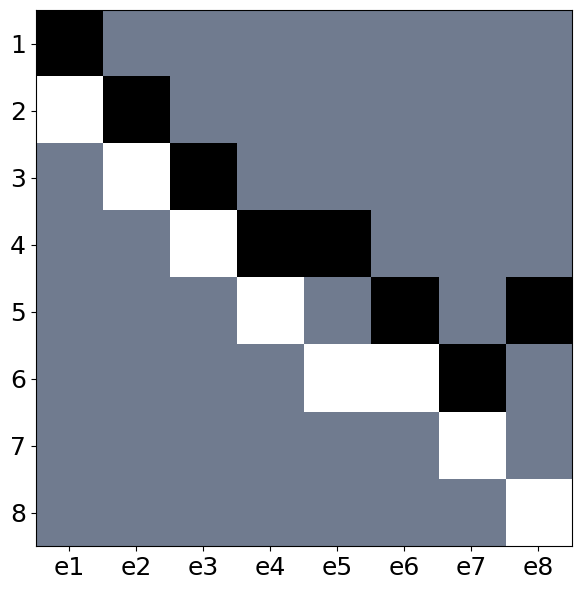
\includegraphics[width=0.65\linewidth]{figures/incidence_matrix.png} 
    \end{minipage}
    
    \vspace{0.3cm}
    \textbf{Objective:} Achieve near-optimizer accuracy with significant runtime reduction.
\end{frame}


\begin{frame}{Optimization Problem: Objective and Constraints}
\footnotesize
The gas network consists of wells $\mathcal{W}$ (supply nodes), pipelines $\mathcal{P}$, compressors $\mathcal{C}$ and unsupplied demand $\mathcal{U}$ (demand nodes) 

\[
\min_{\mathcal{P}, \mathcal{F}} 
\sum_{w \in \mathcal{W}} C_{w} f_{w} +
\sum_{p \in \mathcal{P}} C_{p} f_{p} +
\sum_{c \in \mathcal{C}} C_{c} f_{c} +
\sum_{u \in \mathcal{U}} C_{u} f_{u}
\]
where $C_i$ is the cost per unit flow at element $i$, and $f_i$ is the corresponding gas flow.

\begin{align}
    \underline{f_{w}} \leq f_{w} \leq \overline{f_{w}} 
    &\quad \forall \ w \in \mathcal{W} 
    &&\parbox{3cm}{\centering Well capacity} \label{eq:well_limits} \\
    -\overline{f_{p}} \leq f_{p} \leq \overline{f_{p}} 
    &\quad \forall \ p \in \mathcal{P} 
    &&\parbox{3cm}{\centering Pipeline limits} \label{eq:pipe_limits} \\
    0 \leq f_{u} \leq \overline{f_{u}} 
    &\quad \forall \ u \in \mathcal{U} 
    &&\parbox{3cm}{\centering Demand satisfaction} \label{eq:dem_limit_gas} \\
    \sum_{m:(m,n)\in\mathcal{A}} f_{m} 
    &= \sum_{m':(n,m')\in\mathcal{A}} f_{m'} 
    &&\parbox{3cm}{\centering Nodal gas balance} \label{eq:gas_balance}
\end{align}
\end{frame}


\begin{frame}{CensNet Layers: Integrating Node \& Edge Features}
\footnotesize
\textbf{Motivation:}  
Traditional GCNs focus mainly on \textit{node features} and ignore \textit{edge features}, missing part of the graph’s information.

\medskip
\textbf{CensNet innovation:}
\begin{itemize}
    \item Alternates between \textbf{node layers} and \textbf{edge layers}.
    \item Each layer type updates its own features while using information from the other:
    \begin{itemize}
        \item \footnotesize \textbf{Node layer:} Node embeddings are updated using both node adjacency and transformed edge features.
        \item \footnotesize \textbf{Edge layer:} Edge embeddings are updated using edge adjacency and transformed node features.
    \end{itemize}
    \item Uses an \textit{incidence matrix} \( \mathbf{T} \) to pivot between node and edge domains.
\end{itemize}

\medskip
\textbf{Benefits:}
\begin{itemize}
    \item Captures both \textit{structural} (adjacency) and \textit{relational} (edge) information.
    \item Enhances long-range dependencies through alternating propagation.
\end{itemize}
\end{frame}


\begin{frame}{Node layer propagation}
\footnotesize

\[
\mathbf{H}_v^{(l+1)} \;=\; \sigma\Big(
\big( \mathbf{T}\,\Phi(\mathbf{H}_e^{(l)}\mathbf{p}_e)\,\mathbf{T}^\top \;\odot\; \tilde{\mathbf{A}}_v \big)
\; \big(\mathbf{H}_v^{(l)} \mathbf{W}_v \big)
\Big)
\]

\vspace{0.5cm}

\textbf{Definitions:}
\begin{itemize}\footnotesize
    \item \(N_v\): number of nodes.
    \item \(D_v, D_v'\): input and output node feature dimensions.
    \item \(\mathbf{H}_v^{(l)} \in \mathbb{R}^{N_v \times D_v}\): node features at layer \(l\).
    \item \(\mathbf{H}_e^{(l)} \in \mathbb{R}^{N_e \times D_e}\): edge features at layer \(l\).
    \item \(\mathbf{p}_e \in \mathbb{R}^{D_e}\): learnable projection vector for edges.
    \item \(\mathbf{T} \in \{0,1\}^{N_v \times N_e}\): incidence matrix.
    \item \(\tilde{\mathbf{A}}_v \in \mathbb{R}^{N_v \times N_v}\): normalized node adjacency.
    \item \(\mathbf{W}_v \in \mathbb{R}^{D_v \times D_v'}\): learnable weight matrix.
    \item \(\sigma(\cdot)\): non-linear activation, applied element-wise.
    \item \(\Phi(\cdot)\): diagonalization operator.
\end{itemize}
\end{frame}


\begin{frame}{Edge layer propagation}
\footnotesize

\[
\mathbf{H}_e^{(l+1)} \;=\; \sigma\Big(
\big( \mathbf{T}^\top \,\Phi(\mathbf{H}_v^{(l)}\mathbf{p}_v)\,\mathbf{T} \;\odot\; \tilde{\mathbf{A}}_e \big)
\; \big(\mathbf{H}_e^{(l)} \mathbf{W}_e \big)
\Big)
\]

\vspace{0.5cm}

\textbf{Definitions:}
\begin{itemize}\footnotesize
    \item \(N_e\): number of edges.
    \item \(D_e, D_e'\): input and output edge feature dimensions.
    \item \(\mathbf{H}_e^{(l)} \in \mathbb{R}^{N_e \times D_e}\): edge features at layer \(l\).
    \item \(\mathbf{H}_v^{(l)} \in \mathbb{R}^{N_v \times D_v}\): node features at layer \(l\).
    \item \(\mathbf{p}_v \in \mathbb{R}^{D_v}\): learnable projection vector for nodes.
    \item \(\tilde{\mathbf{A}}_e \in \mathbb{R}^{N_e \times N_e}\): normalized edge adjacency (line graph).
    \item \(\mathbf{W}_e \in \mathbb{R}^{D_e \times D_e'}\): learnable weight matrix.
    \item \(\sigma(\cdot)\): non-linear activation, applied element-wise.
\end{itemize}
\textbf{Core idea:} Information “pivots” between node and edge spaces at each step, enriching representations.

\end{frame}

\begin{frame}{CensNet-based Model Architecture}
\scriptsize
\justifying
    \centering
    \resizebox{0.9\textwidth}{!}{%
        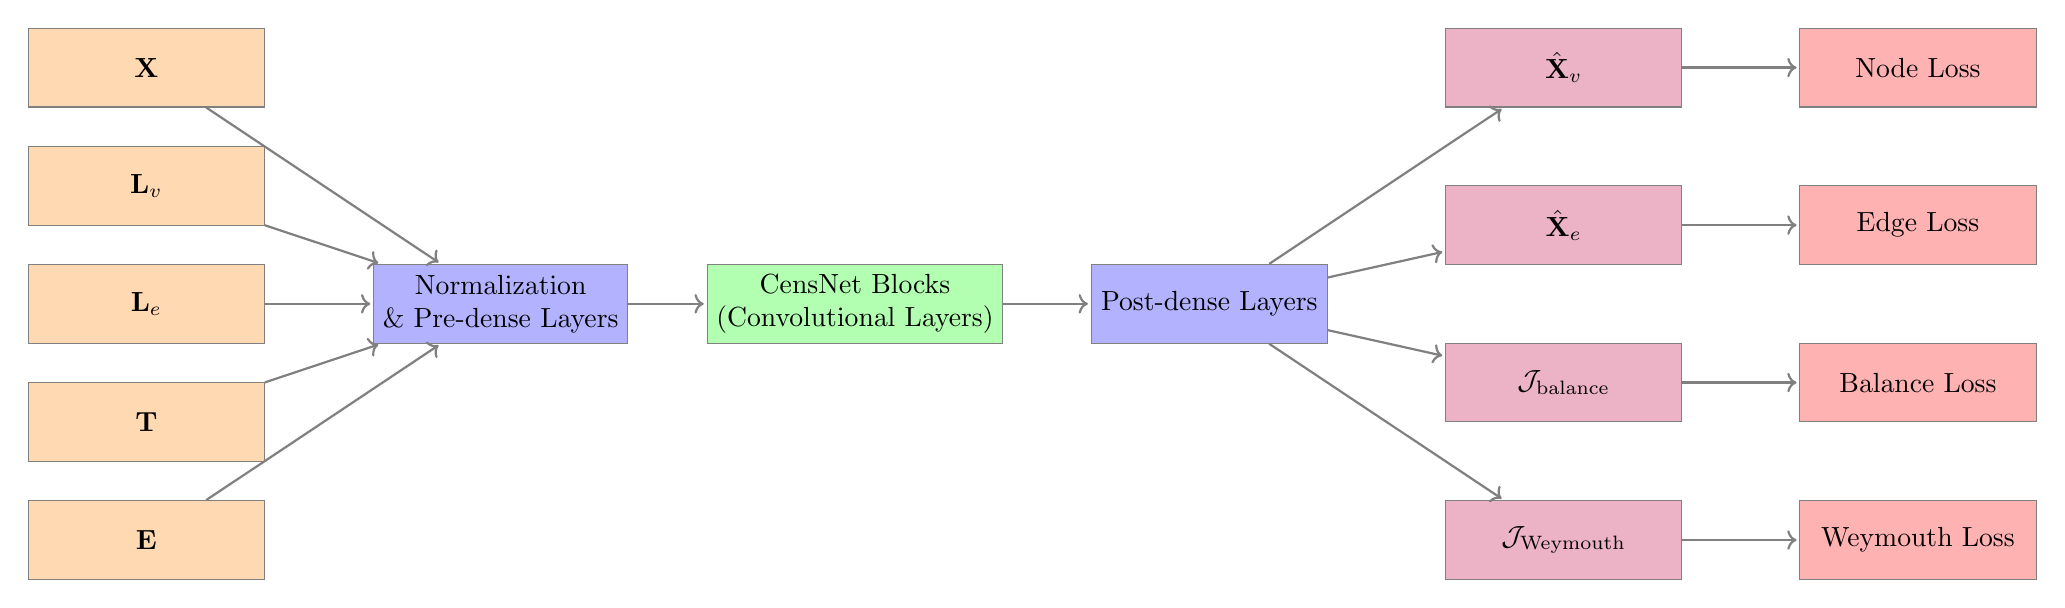
\begin{tikzpicture}[shorten >=1pt, ->, draw=black!50, node distance=1.5cm and 3.5cm, align=center]

    % Styles
    \tikzstyle{input} = [rectangle, draw, fill=orange!30, minimum width=3cm, minimum height=1cm]
    \tikzstyle{dense} = [rectangle, draw, fill=blue!30, minimum width=3cm, minimum height=1cm]
    \tikzstyle{conv} = [rectangle, draw, fill=green!30, minimum width=3cm, minimum height=1cm]
    \tikzstyle{output} = [rectangle, draw, fill=purple!30, minimum width=3cm, minimum height=1cm]
    \tikzstyle{loss} = [rectangle, draw, fill=red!30, minimum width=3cm, minimum height=1cm]
    \tikzstyle{arrow} = [->, thick]

    % Input Layer
    \node[input] (node_features) at (0,0) {\(\mathbf{X}\)};
    \node[input] (node_laplacian) [below of=node_features] {\(\mathbf{L}_v\)};
    \node[input] (edge_laplacian) [below of=node_laplacian] {\(\mathbf{L}_e\)};
    \node[input] (incidence_matrix) [below of=edge_laplacian] {\(\mathbf{T}\)};
    \node[input] (edge_features) [below of=incidence_matrix] {\(\mathbf{E}\)};

    % Normalization and Pre-dense Layer
    \node[dense] (norm_pre_dense) [right of=edge_laplacian, xshift=3cm] {Normalization \\ \& Pre-dense Layers};

    % Convolutional Layers
    \node[conv] (conv_layers) [right of=norm_pre_dense, xshift=3cm] {CensNet Blocks \\ (Convolutional Layers)};

    % Post-dense Layer
    \node[dense] (post_dense) [right of=conv_layers, xshift=3cm] {Post-dense Layers};

    % Outputs
    \node[output] (node_output) [right of=post_dense, xshift=3cm, yshift=3cm] {\(\hat{\mathbf{X}}_v\)};
    \node[output] (edge_output) [right of=post_dense, xshift=3cm, yshift=1cm] {\(\hat{\mathbf{X}}_e\)};
    \node[output] (balance_output) [right of=post_dense, xshift=3cm, yshift=-1cm] {\(\mathcal{J}_{\text{balance}}\)};
    \node[output] (weymouth_output) [right of=post_dense, xshift=3cm, yshift=-3cm] {\(\mathcal{J}_{\text{Weymouth}}\)};

    % Losses
    \node[loss] (node_loss) [right of=node_output, xshift=3cm] {Node Loss};
    \node[loss] (edge_loss) [right of=edge_output, xshift=3cm] {Edge Loss};
    \node[loss] (balance_loss) [right of=balance_output, xshift=3cm] {Balance Loss};
    \node[loss] (weymouth_loss) [right of=weymouth_output, xshift=3cm] {Weymouth Loss};

    % Arrows
    \draw[arrow] (node_features) -- (norm_pre_dense);
    \draw[arrow] (node_laplacian) -- (norm_pre_dense);
    \draw[arrow] (edge_laplacian) -- (norm_pre_dense);
    \draw[arrow] (incidence_matrix) -- (norm_pre_dense);
    \draw[arrow] (edge_features) -- (norm_pre_dense);

    \draw[arrow] (norm_pre_dense) -- (conv_layers);
    \draw[arrow] (conv_layers) -- (post_dense);

    \draw[arrow] (post_dense) -- (node_output);
    \draw[arrow] (post_dense) -- (edge_output);
    \draw[arrow] (post_dense) -- (balance_output);
    \draw[arrow] (post_dense) -- (weymouth_output);

    \draw[arrow] (node_output) -- (node_loss);
    \draw[arrow] (edge_output) -- (edge_loss);
    \draw[arrow] (balance_output) -- (balance_loss);
    \draw[arrow] (weymouth_output) -- (weymouth_loss);

\end{tikzpicture}

%
    } 

\vspace{0.2cm}
\textbf{Inputs:} Encapsulate both physical attributes and topological information of the network:
\begin{itemize}
    \item \footnotesize Node features: 
    \(\mathbf{X} \in \mathbb{R}^{N_v \times 3}\),  
    injection limits and demand. 
    
    \item \footnotesize Node Laplacian: 
    \(\mathbf{L}_v \in \mathbb{R}^{N_v \times N_v}\),  
    node connectivity. 
    
    \item \footnotesize Edge Laplacian: 
    \(\mathbf{L}_e \in \mathbb{R}^{N_e \times N_e}\),  
    edge connectivity. 
    
    \item \footnotesize Edge features: 
    \(\mathbf{E} \in \mathbb{R}^{N_e \times 5}\),  
    \(K\), \(\beta\), flow limits. 
\end{itemize}

\[
    \mathcal{L}(\Theta) = 
    \sum_{r=1}^{R} 
    \Big(
    \| \mathbf{X}_{v,r} - \hat{\mathbf{X}}_{v,r} \|_2^2 +
    \| \mathbf{X}_{e,r} - \hat{\mathbf{X}}_{e,r} \|_2^2
    \Big)
\]
\end{frame}


\begin{frame}{Dataset and Experimental Setup}
\scriptsize
\begin{columns}[t,onlytextwidth]
    \begin{column}{0.55\textwidth}
        Two different gas network configurations were used to evaluate the proposed CensNet-based model.

        \vspace{0.3em}
        \begin{table}[H]
            \centering
            \setlength{\tabcolsep}{4pt}
            \renewcommand{\arraystretch}{1.1}
            \begin{tabular}{lcccc}
                \toprule
                \textbf{Case} & \textbf{Nodes} & \textbf{Pipes} & \textbf{Comps.} & \textbf{Users} \\
                \midrule
                8-node & 8  & 6  & 2  & 2  \\
                Colombia & 63 & 48 & 14 & 27 \\
                \bottomrule
            \end{tabular}
        \end{table}

        \vspace{0.5em}
        Different scenarios were generated by adding 5\%–25\% noise to user demands and solving with APOPT.
        These outputs were used as training targets for the CensNet model.
        
         \vspace{1em}

        \textbf{Experimental Setup}
        \begin{itemize}
            \item \textbf{Samples:} 2000 (8-node), 2400 (63-node)
            \item \textbf{Data split:} 60\% train, 20\% val, 20\% test  
        \end{itemize}
    \end{column}

    \begin{column}{0.43\textwidth}
        \scriptsize
        % \textbf{Experimental Setup}
        \begin{itemize}
            \item \textbf{Training:} 1500 epochs, Adam optimizer, Leaky ReLU ($\alpha=0.2$)
            \item \textbf{Learning rate:} $1\times10^{-2}$, exponential decay (0.9 every 1000 steps)
            \item \textbf{Hyperparameters:}
            \begin{itemize}
                \scriptsize
                \item $N_{\text{channels}}$: 16–64
                \item $N_{\text{layers}}$: 1–5 (conv)
                \item $N_{\text{dense}}$: 2–32 (post-dense)
            \end{itemize}
            \item \textbf{Losses tested:}
            \begin{itemize}
                \scriptsize
                \item Nodal loss only
                \item Nodal + edge loss
            \end{itemize}
        \end{itemize}
    \end{column}
\end{columns}
\end{frame}


\begin{frame}{Performance Comparison: 8-Node and 63-Node Networks}
\tiny
\centering
\begin{table}
\captionsetup{font=scriptsize}
\begin{tabular}{lccccc}
\toprule
    \textbf{Model} & \textbf{Nodal $R^2$} & \textbf{Edge $R^2$} & \multicolumn{1}{c}{\textbf{\parbox{2cm}{Balance Error}}} & \textbf{Time (s)} & \textbf{T-test} \\
\midrule
\multicolumn{6}{c}{\textbf{8-node Network}} \\
\midrule
CensNet (N)     & 0.99 & -2.82 & 5.7 \(\pm\) 16.86 & 0.65 \(\pm\) 0.4 & $T=15$\\
CensNet (N+E)   & 0.99 & 0.99  & 0.08 \(\pm\) 1.17 & 0.64 \(\pm\) 0.4 & $p=1.3\times10^{-34}$ \\
\midrule
\multicolumn{6}{c}{\textbf{63-node Network}} \\
\midrule
CensNet (N)     & 0.99  & -5.88 & 0.04 \(\pm\) 60.83 & 4.9 \(\pm\) 5.6 & $T=47$\\
CensNet (N+E)   & 0.99  & 0.99  & 0.01 \(\pm\) 23.4 & 4.9 \(\pm\) 5.6 & $p=4.9\times10^{-110}$ \\
\bottomrule
\end{tabular}
\end{table}

\medskip
\justifying
\scriptsize
The CensNet-based model captures the network’s topological information, allowing it to naturally satisfy the gas balance constraint to some extent. It is also significantly faster than APOPT and can efficiently process entire batches of scenarios
\end{frame}


\section{Objective 2 - Natural Gas System Optimization Using MPCC-Based Models}
\begin{frame}{Objective 2 - Interconnected system - Definition}
A power-gas interconnected system is a hybrid infrastructure that integrates natural gas and power networks, enhancing overall system efficiency~\cite{Duan_Liu_Yang_2022}. 
\begin{columns}
\begin{column}{0.5\textwidth}
   \begin{center}
     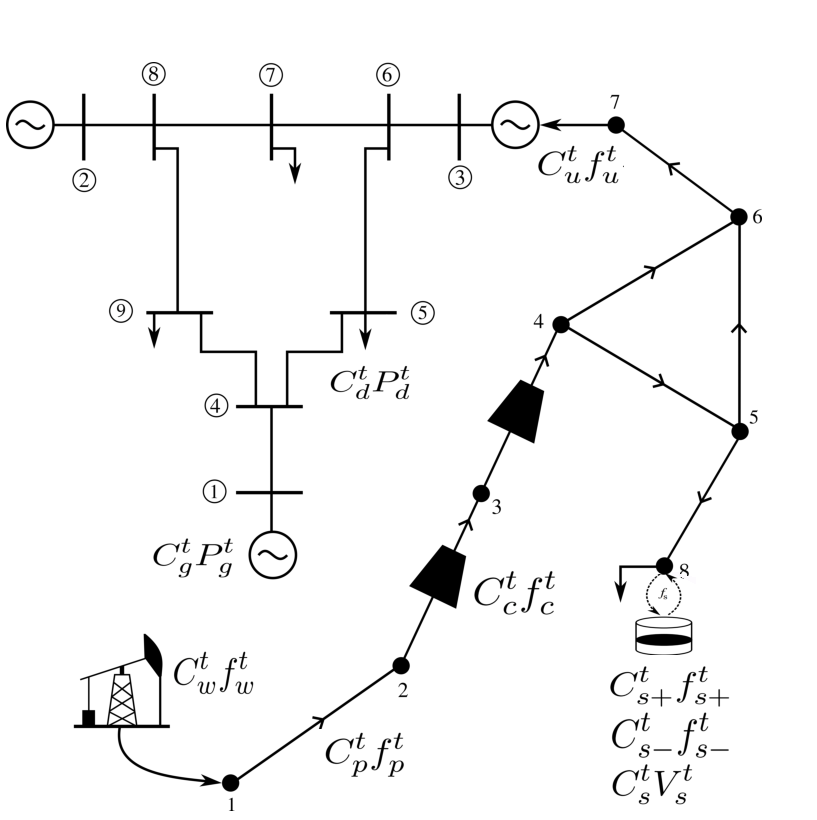
\includegraphics[width=1\textwidth]{figures/network_math_alternative.pdf}
     \end{center}
\end{column}
\begin{column}{0.5\textwidth}  
\begin{equation} \label{eq:obj_func_integrated}
\begin{split}
 \min_{\mathcal{P}, \mathcal{F}} \quad  \sum_{t \in \mathcal{T}} (   \sum_{g \in \mathcal{G}} C_{g}^t {P_{g}^t} + \sum_{d \in \mathcal{D}} C_{d}^t {P_{d}^t} +  \\ \sum_{w \in \mathcal{W}} C_{w}^t {f_{w}^t} +  \sum_{p \in \mathcal{P}} C_{p}^t {f_{p}^t}  + \\ \sum_{c \in \mathcal{C}} C_{c}^t {f_{c}^t} + \sum_{u \in \mathcal{U}} C_{u}^{t} {f_{u}^{t}} + \\ \quad \sum_{s \in \mathcal{S}} C_{s+}^{t} {f_{s+}^{t}}  + \sum_{s \in \mathcal{S}} C_{s-}^{t} {f_{s-}^{t}} + \\ \sum_{s \in \mathcal{S}} C_{s}^{t} {V_{s}^{t}} )
\end{split}
\end{equation} 
\end{column}
\end{columns}
\end{frame}


\begin{frame}{Power system constraints}
\footnotesize
The constraints of the electrical system represent the technical limits of its components, as well as the physical laws that govern them. In this work, the DC model is adopted, which has been shown to be sufficient for similar applications~\cite{8468081}.
\begin{columns}
\begin{column}{0.24\textwidth}
% \begin{center}
\vspace{3pt}
    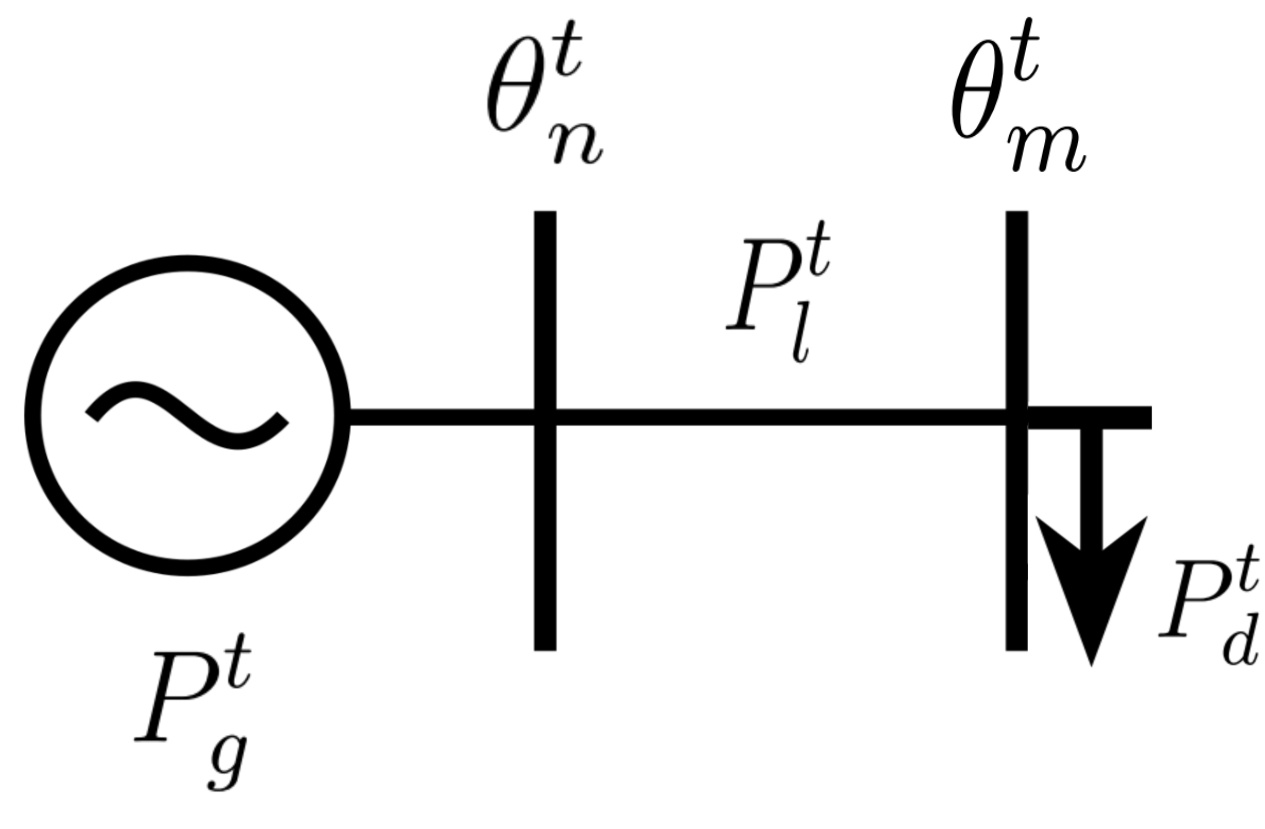
\includegraphics[width=1.4\textwidth]{figures/power_dummy_constraint.png}
% \end{center}
\end{column}
\begin{column}{0.8\textwidth}  %%<--- here


\begin{subequations}
\begin{alignat}{2}
    \underline{P_g^t} \leq P_{g}^t \leq \overline{P_g^t} &\quad &\forall \ g \in \mathcal{G}, \label{eq:gen_limits} \\
    -\overline{P_l^t} \leq P_{l}^t \leq \overline{P_l^t} &\quad &\forall \ l \in \mathcal{L}, \label{eq:line_limits} \\
    P_{l}^t = B_{nm}(\theta_n - \theta_{m}) &\quad &\forall \ l = (n, m) \in \mathcal{L}, \label{eq:dc_power_flow} \\
    0 \leq P_{d}^t \leq \overline{P_{d}^t} &\quad &\forall \ d \in \mathcal{D}, \label{eq:dem_limit_power} \\
    -\overline{\theta_{n}^t} \leq \theta_{m}^t \leq \overline{\theta_{n}^t} &\quad &\forall \ n \in \mathcal{N}_P, \label{eq:voltage_angle_limits} \\
    \sum_{\substack{l\in \mathcal{L}_{n+}\\g=n}}{P_{l}^t + P_{g}^t} = \sum_{\substack{l\in \mathcal{L}_{n-}\\d=n}} P_{l}^t + P_{d}^t &\quad &\forall \ n \in \mathcal{N}_P \label{eq:power_balance}
\end{alignat}
\end{subequations}
\end{column}
\end{columns}

\vspace{1em}
The second set of restrictions interconnects the natural gas and electric power systems through gas-fired power plants that generate electricity.
\begin{align}
    &f_{n}^t = P_{n}^t \cdot \text{HR}_n, \quad \forall \ n \in \mathcal{N}_I, \label{eq:gas_power_relation} 
\end{align}
\end{frame}


\begin{frame}{Gas system constraints}
\footnotesize
This set of constraints ensures that wells, pipelines, nodal pressures, compressors, unsupplied demand and storage facilities operate within proper operating limits.~\cite{MPNG}.

\begin{columns}
\begin{column}{0.5\textwidth}
    \includegraphics[width=0.75\textwidth]{figures/gas_dummy.png}
\end{column}

\begin{column}{0.5\textwidth}
\scriptsize % optional to avoid overfull boxes

\begin{fleqn}[0pt]
\begin{subequations}
\begin{align}
    \pi_{m}^t & \leq \beta_{c}^t{\pi_{n}^t} \quad \forall \ c=(n,m) \in \mathcal{C} \label{eq:comp_ratio} \\
    0  & \leq f_{s+}^t \leq V_{0s} - \underline{V_s} \quad \forall \ s \in \mathcal{S} \label{eq:sto_limit1} \\
    0 & \leq f_{s-}^t \leq \overline{V_s} - V_{0s} \quad \forall \ s \in \mathcal{S} \label{eq:sto_limit2} \\
    V_{s}^t & = V_{s}^{t-1} + f_{s-}^{t-1} - f_{s+}^{t-1} \quad \forall \ s \in \mathcal{S} \label{eq:sto_time}
    \end{align}
\end{subequations}
\end{fleqn}
\end{column}
\end{columns}
\begin{equation}
    \colorboxed[rgb]{0,0,1}{
    \text{sgn}(f_{p}^t)(f_{p}^t)^2 = K_{nm}((\pi_{n}^t)^2 - (\pi_{m}^t)^2) \quad \forall \ p =(n,m) \in \mathcal{P}
    }
\end{equation}
Modeling the Weymouth equation as a nonconvex and discontinuous equality constraint presents significant challenges for optimization algorithms, leading to multiple local optima~\cite{JIANG2021106460}.
\end{frame}


\begin{frame}{Proposed complementarity-based approach}
\footnotesize
Complementarity constraints can be used to represent non-uniform or discontinuous operators, such as absolute value, sign, and min/max \cite{mpcc}. The sign equation can be represented by an optimization problem whose constraints avoid the use of binary variables.


\begin{subequations}
\begin{align}
\mathcal{O}_\epsilon: \quad &\min\limits_{y_p^t} \ -y_p^t f_p^t \label{eq:complementarity_relaxec1} \\
&\text{s.t.} \quad y_p^t (f_p^t)^2 = K_{nm} \left( (\pi_n^t)^2 - (\pi_m^t)^2 \right) \\
&f_p^t = f_{p+}^t - f_{p-}^t \\
&-1 \leq y_p^t \leq 1 \\
&f_{p+}^t (y_p^t + 1) \leq \epsilon \label{eq:Oe:complementarity1} \\
&f_{p-}^t (1 - y_p^t) \leq \epsilon \label{eq:Oe:complementarity2}
\end{align}
\end{subequations}

The regularized optimization model $\mathcal{O}_{\epsilon}$ offers several key properties that justify its use in tackling challenging MPCC problems~\cite{Ralph_Wright_2004}.
\end{frame}



\begin{frame}{Databases}
Each of the mentioned databases was selected based on its unique characteristics and the significant contributions it could make to the study.

\begin{table}[]
\begin{tabular}{|c|c|c|c|c|}
\hline
                & \textbf{Topology}                                           & \textbf{\begin{tabular}[c]{@{}c@{}}Connection \\ points\end{tabular}} & \textbf{\begin{tabular}[c]{@{}c@{}}Closed\\ loops\end{tabular}} & \textbf{Problem}                                                                               \\ \hline
\textbf{Case 1} & \begin{tabular}[c]{@{}c@{}}9-bus\\ 8-system\end{tabular}    & 1                                                                          & 1                                                                      & \begin{tabular}[c]{@{}c@{}}Small system\\ with one loop\end{tabular}                           \\ \hline
\textbf{Case 2} & \begin{tabular}[c]{@{}c@{}}118-bus\\ 48-system\end{tabular} & 9                                                                          & 7                                                                      & \begin{tabular}[c]{@{}c@{}}Contains several\\ interconnected \\ loops\end{tabular}             \\ \hline
\textbf{Case 3} & \begin{tabular}[c]{@{}c@{}}96-bus\\ 63-system\end{tabular}  & 10                                                                         & 0                                                                      & \begin{tabular}[c]{@{}c@{}}Fully radial \\ but considers  \\ bidirectional flows.\end{tabular} \\ \hline
\end{tabular}
\label{tab:databases}
\end{table}
\end{frame}



\begin{frame}{Experimental setup}
\footnotesize
In order to establish a baseline for comparison, two alternative methodologies were employed: 
\begin{itemize}
    \item Taylor series approximation \cite{taylor_paper}.
    \item Second Order Cone Programming (SOC) \cite{soc_paper}.
\end{itemize}

The objective function value for each of the mentioned databases was computed by solving the optimization problem using: 
\begin{itemize}
    \item The IPOPT \cite{ipopt} solver.
    \item The GEKKO \cite{gekko} package. 
\end{itemize}

Since understanding and quantifying the inherent errors introduced by any constraint approximation approach supports its real-world pertinence, the considered validation trades off the reached cost function and constraint error values.

    \begin{equation}
    {WE}_p^t = |f_{p}^t - \left(K_{nm}|(\pi_{n}^t)^2-(\pi_{m}^t)^2|\right)^{1/2}| , \quad \forall \ p =(n,m) \in\mathcal{P}
\end{equation}
Hence, ${WE}_p^t$ metric explains the inherent sensitivity of tested approaches and validates the significance of their differences.

\end{frame}


\begin{frame}{Results - Case 1}
\scriptsize
\begin{columns}[t,onlytextwidth]
    \begin{column}{0.48\textwidth} 
        \justifying
        The optimization problem was solved one hundred times for a single day, using a Monte Carlo experiment with uniformly sampled gas demands.       
        \vspace{0.5em}
        \begin{figure}[!htb]
            \centering
            \setlength\figurewidth{1\textwidth}        
            \setlength\figureheight{0.9\textwidth}
            % This file was created with tikzplotlib v0.10.1.
\begin{tikzpicture}

\definecolor{darkgray176}{RGB}{176,176,176}
\definecolor{darkorange25512714}{RGB}{0,0,255}%{255,127,14}
% \definecolor{red}{RGB}{255,0,0}%{44,160,44}
\definecolor{lightgray204}{RGB}{204,204,204}
\definecolor{steelblue31119180}{RGB}{0,128,0}%{31,119,180}

\definecolor{red}{RGB}{255,127,14}
\definecolor{darkorange25512714}{RGB}{44,160,44}
\definecolor{steelblue31119180}{RGB}{31,119,180}
% \definecolor{darkgray176}{RGB}{176,176,176}
% \definecolor{darkorange25512714}{RGB}{255,127,14}
% \definecolor{green}{RGB}{0,128,0}

\begin{axis}[
width=\figurewidth,
height=\figureheight,
legend cell align={left},
legend style={fill opacity=0.8, draw opacity=1, text opacity=1, draw=lightgray204},
tick align=inside,
tick pos=left,
x grid style={darkgray176},
xlabel={Objective function cost},
xmin=5.56829803705899, xmax=8.71309423956304,
xtick style={color=black},
xtick={6,7,8},
xticklabels={
  \(\displaystyle {10^{6}}\),
  \(\displaystyle {10^{7}}\),
  \(\displaystyle {10^{8}}\),
},
xmajorgrids,
y grid style={darkgray176},
ymajorgrids,
ylabel=Relative Frequency,
ymin=0, ymax=29.4,
ytick style={color=black},
ytick={5,15,25},
yticklabels={
  \(\displaystyle {5\%}\),
  \(\displaystyle {15\%}\),
  \(\displaystyle {25\%}\),
},
]
\draw[draw=red,fill=red,fill opacity=0.75,line width=0.195771585198722pt] (axis cs:5.79744147894999,0) rectangle (axis cs:5.84054055892949,28);
\draw[draw=red,fill=red,fill opacity=0.75,line width=0.195771585198722pt] (axis cs:5.94110507888165,0) rectangle (axis cs:5.98420415886115,0);
\draw[draw=red,fill=red,fill opacity=0.75,line width=0.195771585198722pt] (axis cs:6.08476867881331,0) rectangle (axis cs:6.12786775879281,0);
\draw[draw=red,fill=red,fill opacity=0.75,line width=0.195771585198722pt] (axis cs:6.22843227874497,0) rectangle (axis cs:6.27153135872447,0);
\draw[draw=red,fill=red,fill opacity=0.75,line width=0.195771585198722pt] (axis cs:6.37209587867663,0) rectangle (axis cs:6.41519495865613,0);
\draw[draw=red,fill=red,fill opacity=0.75,line width=0.195771585198722pt] (axis cs:6.51575947860829,0) rectangle (axis cs:6.55885855858779,0);
\draw[draw=red,fill=red,fill opacity=0.75,line width=0.195771585198722pt] (axis cs:6.65942307853996,0) rectangle (axis cs:6.70252215851945,0);
\draw[draw=red,fill=red,fill opacity=0.75,line width=0.195771585198722pt] (axis cs:6.80308667847162,0) rectangle (axis cs:6.84618575845111,0);
\draw[draw=red,fill=red,fill opacity=0.75,line width=0.195771585198722pt] (axis cs:6.94675027840328,0) rectangle (axis cs:6.98984935838278,0);
\draw[draw=red,fill=red,fill opacity=0.75,line width=0.195771585198722pt] (axis cs:7.09041387833494,0) rectangle (axis cs:7.13351295831444,1);
\draw[draw=red,fill=red,fill opacity=0.75,line width=0.195771585198722pt] (axis cs:7.2340774782666,0) rectangle (axis cs:7.2771765582461,1);
\draw[draw=red,fill=red,fill opacity=0.75,line width=0.195771585198722pt] (axis cs:7.37774107819826,0) rectangle (axis cs:7.42084015817776,0);
\draw[draw=red,fill=red,fill opacity=0.75,line width=0.195771585198722pt] (axis cs:7.52140467812992,0) rectangle (axis cs:7.56450375810942,2);
\draw[draw=red,fill=red,fill opacity=0.75,line width=0.195771585198722pt] (axis cs:7.66506827806158,0) rectangle (axis cs:7.70816735804108,2);
\draw[draw=red,fill=red,fill opacity=0.75,line width=0.195771585198722pt] (axis cs:7.80873187799324,0) rectangle (axis cs:7.85183095797274,3);
\draw[draw=red,fill=red,fill opacity=0.75,line width=0.195771585198722pt] (axis cs:7.9523954779249,0) rectangle (axis cs:7.9954945579044,1);
\draw[draw=red,fill=red,fill opacity=0.75,line width=0.195771585198722pt] (axis cs:8.09605907785656,0) rectangle (axis cs:8.13915815783606,8);
\draw[draw=red,fill=red,fill opacity=0.75,line width=0.195771585198722pt] (axis cs:8.23972267778822,0) rectangle (axis cs:8.28282175776772,12);
\draw[draw=red,fill=red,fill opacity=0.75,line width=0.195771585198722pt] (axis cs:8.38338627771988,0) rectangle (axis cs:8.42648535769938,18);
\draw[draw=red,fill=red,fill opacity=0.75,line width=0.195771585198722pt] (axis cs:8.52704987765154,0) rectangle (axis cs:8.57014895763104,12);
\draw[draw=darkorange25512714,fill=darkorange25512714,fill opacity=0.75,line width=0.195771585198722pt] (axis cs:5.75434239897049,0) rectangle (axis cs:5.79744147894999,28);
\draw[draw=darkorange25512714,fill=darkorange25512714,fill opacity=0.75,line width=0.195771585198722pt] (axis cs:5.89800599890215,0) rectangle (axis cs:5.94110507888165,0);
\draw[draw=darkorange25512714,fill=darkorange25512714,fill opacity=0.75,line width=0.195771585198722pt] (axis cs:6.04166959883381,0) rectangle (axis cs:6.08476867881331,0);
\draw[draw=darkorange25512714,fill=darkorange25512714,fill opacity=0.75,line width=0.195771585198722pt] (axis cs:6.18533319876548,0) rectangle (axis cs:6.22843227874497,0);
\draw[draw=darkorange25512714,fill=darkorange25512714,fill opacity=0.75,line width=0.195771585198722pt] (axis cs:6.32899679869714,0) rectangle (axis cs:6.37209587867663,0);
\draw[draw=darkorange25512714,fill=darkorange25512714,fill opacity=0.75,line width=0.195771585198722pt] (axis cs:6.4726603986288,0) rectangle (axis cs:6.51575947860829,0);
\draw[draw=darkorange25512714,fill=darkorange25512714,fill opacity=0.75,line width=0.195771585198722pt] (axis cs:6.61632399856046,0) rectangle (axis cs:6.65942307853996,0);
\draw[draw=darkorange25512714,fill=darkorange25512714,fill opacity=0.75,line width=0.195771585198722pt] (axis cs:6.75998759849212,0) rectangle (axis cs:6.80308667847162,0);
\draw[draw=darkorange25512714,fill=darkorange25512714,fill opacity=0.75,line width=0.195771585198722pt] (axis cs:6.90365119842378,0) rectangle (axis cs:6.94675027840328,0);
\draw[draw=darkorange25512714,fill=darkorange25512714,fill opacity=0.75,line width=0.195771585198722pt] (axis cs:7.04731479835544,0) rectangle (axis cs:7.09041387833494,1);
\draw[draw=darkorange25512714,fill=darkorange25512714,fill opacity=0.75,line width=0.195771585198722pt] (axis cs:7.1909783982871,0) rectangle (axis cs:7.2340774782666,1);
\draw[draw=darkorange25512714,fill=darkorange25512714,fill opacity=0.75,line width=0.195771585198722pt] (axis cs:7.33464199821876,0) rectangle (axis cs:7.37774107819826,0);
\draw[draw=darkorange25512714,fill=darkorange25512714,fill opacity=0.75,line width=0.195771585198722pt] (axis cs:7.47830559815042,0) rectangle (axis cs:7.52140467812992,2);
\draw[draw=darkorange25512714,fill=darkorange25512714,fill opacity=0.75,line width=0.195771585198722pt] (axis cs:7.62196919808208,0) rectangle (axis cs:7.66506827806158,2);
\draw[draw=darkorange25512714,fill=darkorange25512714,fill opacity=0.75,line width=0.195771585198722pt] (axis cs:7.76563279801374,0) rectangle (axis cs:7.80873187799324,3);
\draw[draw=darkorange25512714,fill=darkorange25512714,fill opacity=0.75,line width=0.195771585198722pt] (axis cs:7.9092963979454,0) rectangle (axis cs:7.9523954779249,1);
\draw[draw=darkorange25512714,fill=darkorange25512714,fill opacity=0.75,line width=0.195771585198722pt] (axis cs:8.05295999787706,0) rectangle (axis cs:8.09605907785656,8);
\draw[draw=darkorange25512714,fill=darkorange25512714,fill opacity=0.75,line width=0.195771585198722pt] (axis cs:8.19662359780873,0) rectangle (axis cs:8.23972267778822,12);
\draw[draw=darkorange25512714,fill=darkorange25512714,fill opacity=0.75,line width=0.195771585198722pt] (axis cs:8.34028719774039,0) rectangle (axis cs:8.38338627771988,18);
\draw[draw=darkorange25512714,fill=darkorange25512714,fill opacity=0.75,line width=0.195771585198722pt] (axis cs:8.48395079767205,0) rectangle (axis cs:8.52704987765154,12);
\draw[draw=steelblue31119180,fill=steelblue31119180,fill opacity=0.75,line width=0.195771585198722pt] (axis cs:5.71124331899099,0) rectangle (axis cs:5.75434239897049,28);
\draw[draw=steelblue31119180,fill=steelblue31119180,fill opacity=0.75,line width=0.195771585198722pt] (axis cs:5.85490691892266,0) rectangle (axis cs:5.89800599890215,0);
\draw[draw=steelblue31119180,fill=steelblue31119180,fill opacity=0.75,line width=0.195771585198722pt] (axis cs:5.99857051885432,0) rectangle (axis cs:6.04166959883381,0);
\draw[draw=steelblue31119180,fill=steelblue31119180,fill opacity=0.75,line width=0.195771585198722pt] (axis cs:6.14223411878598,0) rectangle (axis cs:6.18533319876548,0);
\draw[draw=steelblue31119180,fill=steelblue31119180,fill opacity=0.75,line width=0.195771585198722pt] (axis cs:6.28589771871764,0) rectangle (axis cs:6.32899679869714,0);
\draw[draw=steelblue31119180,fill=steelblue31119180,fill opacity=0.75,line width=0.195771585198722pt] (axis cs:6.4295613186493,0) rectangle (axis cs:6.4726603986288,0);
\draw[draw=steelblue31119180,fill=steelblue31119180,fill opacity=0.75,line width=0.195771585198722pt] (axis cs:6.57322491858096,0) rectangle (axis cs:6.61632399856046,0);
\draw[draw=steelblue31119180,fill=steelblue31119180,fill opacity=0.75,line width=0.195771585198722pt] (axis cs:6.71688851851262,0) rectangle (axis cs:6.75998759849212,0);
\draw[draw=steelblue31119180,fill=steelblue31119180,fill opacity=0.75,line width=0.195771585198722pt] (axis cs:6.86055211844428,0) rectangle (axis cs:6.90365119842378,0);
\draw[draw=steelblue31119180,fill=steelblue31119180,fill opacity=0.75,line width=0.195771585198722pt] (axis cs:7.00421571837594,0) rectangle (axis cs:7.04731479835544,1);
\draw[draw=steelblue31119180,fill=steelblue31119180,fill opacity=0.75,line width=0.195771585198722pt] (axis cs:7.1478793183076,0) rectangle (axis cs:7.1909783982871,1);
\draw[draw=steelblue31119180,fill=steelblue31119180,fill opacity=0.75,line width=0.195771585198722pt] (axis cs:7.29154291823926,0) rectangle (axis cs:7.33464199821876,0);
\draw[draw=steelblue31119180,fill=steelblue31119180,fill opacity=0.75,line width=0.195771585198722pt] (axis cs:7.43520651817092,0) rectangle (axis cs:7.47830559815042,2);
\draw[draw=steelblue31119180,fill=steelblue31119180,fill opacity=0.75,line width=0.195771585198722pt] (axis cs:7.57887011810258,0) rectangle (axis cs:7.62196919808208,2);
\draw[draw=steelblue31119180,fill=steelblue31119180,fill opacity=0.75,line width=0.195771585198722pt] (axis cs:7.72253371803424,0) rectangle (axis cs:7.76563279801374,3);
\draw[draw=steelblue31119180,fill=steelblue31119180,fill opacity=0.75,line width=0.195771585198722pt] (axis cs:7.86619731796591,0) rectangle (axis cs:7.9092963979454,1);
\draw[draw=steelblue31119180,fill=steelblue31119180,fill opacity=0.75,line width=0.195771585198722pt] (axis cs:8.00986091789756,0) rectangle (axis cs:8.05295999787706,8);
\draw[draw=steelblue31119180,fill=steelblue31119180,fill opacity=0.75,line width=0.195771585198722pt] (axis cs:8.15352451782923,0) rectangle (axis cs:8.19662359780873,12);
\draw[draw=steelblue31119180,fill=steelblue31119180,fill opacity=0.75,line width=0.195771585198722pt] (axis cs:8.29718811776089,0) rectangle (axis cs:8.34028719774039,18);
\draw[draw=steelblue31119180,fill=steelblue31119180,fill opacity=0.75,line width=0.195771585198722pt] (axis cs:8.44085171769255,0) rectangle (axis cs:8.48395079767205,12);


\node[draw,fill=white,anchor=north east] at (axis description cs:0.735,0.97) {
    \begin{tabular}{@{}cl}
        \tikz\draw[steelblue31119180,fill=steelblue31119180] (0,0) rectangle (15,5); & Taylor \\
        \tikz\draw[darkorange25512714,fill=darkorange25512714] (0,0) rectangle (15,5); & SOC \\
        \tikz\draw[red,fill=red] (0,0) rectangle (15,5); & MPCC \\
    \end{tabular}
};

\end{axis}

\end{tikzpicture}

            \label{fig:blue_test_cost}
\end{figure}
    \end{column}
    
    \begin{column}{0.48\textwidth}
        \justifying
        The error distributions shows that the complementarity-based formulation (MPCC) produces considerably lower deviations in key arcs compared to the Taylor and SOC approaches.
        \vspace{2.5em}
        \begin{figure}[!htb]
            \centering
            \setlength\figurewidth{1\textwidth}        
            \setlength\figureheight{0.9\textwidth}
            % This file was created with tikzplotlib v0.10.1.
\begin{tikzpicture}



\definecolor{darkgray176}{RGB}{176,176,176}
\definecolor{darkorange25512714}{RGB}{255,127,14}
\definecolor{green}{RGB}{0,128,0}

\definecolor{red}{RGB}{255,127,14}
\definecolor{blue}{RGB}{44,160,44}
\definecolor{green}{RGB}{31,119,180}
% \definecolor{darkgray176}{RGB}{176,176,176}
% \definecolor{darkorange25512714}{RGB}{255,127,14}
% \definecolor{green}{RGB}{0,128,0}
% \definecolor{blue}{RGB}{0,0,255}
% \definecolor{red}{RGB}{255,0,0}

\begin{axis}[
width=\figurewidth,
height=\figureheight,
log basis y={10},
tick align=inside,
tick pos=left,
title={},
x grid style={darkgray176},
xlabel=\textcolor{black}{},
xmajorgrids,
xmin=0.7, xmax=7.1,
xlabel=\textcolor{black}{Pipeline $p$},
xtick style={color=black},
xtick={1.3,2.3,3.3,4.3,5.3,6.3},
% xticklabels={Pipeline 1,Pipeline 2,Pipeline 3,Pipeline 4,Pipeline 5,Pipeline 6},
xticklabels={1, 2, 3, 4, 5, 6},
y grid style={darkgray176},
ylabel=\textcolor{black}{Weymouth Error ${WE}_p^t$},
ymajorgrids,
ymin=8.03062306955492e-21, ymax=2273681.58974515,
ymode=log,
ytick style={color=black},
ytick={1e-25,1e-21,1e-17,1e-13,1e-09,1e-05,0.1,1000,10000000,100000000000},
yticklabels={
  \(\displaystyle {10^{-27}}\),
  \(\displaystyle {10^{-23}}\),
  \(\displaystyle {10^{-19}}\),
  \(\displaystyle {10^{-15}}\),
  \(\displaystyle {10^{-11}}\),
  \(\displaystyle {10^{-7}}\),
  \(\displaystyle {10^{-3}}\),
  \(\displaystyle {10^{1}}\),
  \(\displaystyle {10^{5}}\),
  \(\displaystyle {10^{9}}\)
}
]
\path [draw=black, fill=green]
(axis cs:1.125,137823.161990151)
--(axis cs:1.275,137823.161990151)
--(axis cs:1.275,139906.555504498)
--(axis cs:1.125,139906.555504498)
--(axis cs:1.125,137823.161990151)
--cycle;
\addplot [black]
table {%
1.2 137823.161990151
1.2 136054.028730085
};
\addplot [black]
table {%
1.2 139906.555504498
1.2 142224.57617864
};
\addplot [black]
table {%
1.1625 136054.028730085
1.2375 136054.028730085
};
\addplot [black]
table {%
1.1625 142224.57617864
1.2375 142224.57617864
};
\path [draw=black, fill=green]
(axis cs:2.125,7055.82777026869)
--(axis cs:2.275,7055.82777026869)
--(axis cs:2.275,7452.89592103251)
--(axis cs:2.125,7452.89592103251)
--(axis cs:2.125,7055.82777026869)
--cycle;
\addplot [black]
table {%
2.2 7055.82777026869
2.2 6557.98366270705
};
\addplot [black]
table {%
2.2 7452.89592103251
2.2 7622.53153112651
};
\addplot [black]
table {%
2.1625 6557.98366270705
2.2375 6557.98366270705
};
\addplot [black]
table {%
2.1625 7622.53153112651
2.2375 7622.53153112651
};
\path [draw=black, fill=green]
(axis cs:3.125,9330.66201749973)
--(axis cs:3.275,9330.66201749973)
--(axis cs:3.275,9656.37935568632)
--(axis cs:3.125,9656.37935568632)
--(axis cs:3.125,9330.66201749973)
--cycle;
\addplot [black]
table {%
3.2 9330.66201749973
3.2 8986.80574615905
};
\addplot [black]
table {%
3.2 9656.37935568632
3.2 10037.0411221129
};
\addplot [black]
table {%
3.1625 8986.80574615905
3.2375 8986.80574615905
};
\addplot [black]
table {%
3.1625 10037.0411221129
3.2375 10037.0411221129
};
\path [draw=black, fill=green]
(axis cs:4.125,7.00639709830284e-06)
--(axis cs:4.275,7.00639709830284e-06)
--(axis cs:4.275,11.075896632379)
--(axis cs:4.125,11.075896632379)
--(axis cs:4.125,7.00639709830284e-06)
--cycle;
\addplot [black]
table {%
4.2 7.00639709830284e-06
4.2 4.37899818643928e-06
};
\addplot [black]
table {%
4.2 11.075896632379
4.2 24.5389341347034
};
\addplot [black]
table {%
4.1625 4.37899818643928e-06
4.2375 4.37899818643928e-06
};
\addplot [black]
table {%
4.1625 24.5389341347034
4.2375 24.5389341347034
};
\path [draw=black, fill=green]
(axis cs:5.125,0.000315145774710587)
--(axis cs:5.275,0.000315145774710587)
--(axis cs:5.275,121.32725197523)
--(axis cs:5.125,121.32725197523)
--(axis cs:5.125,0.000315145774710587)
--cycle;
\addplot [black]
table {%
5.2 0.000315145774710587
5.2 0.000128730853471229
};
\addplot [black]
table {%
5.2 121.32725197523
5.2 291.735233190312
};
\addplot [black]
table {%
5.1625 0.000128730853471229
5.2375 0.000128730853471229
};
\addplot [black]
table {%
5.1625 291.735233190312
5.2375 291.735233190312
};
\path [draw=black, fill=green]
(axis cs:6.125,2.42895564973857)
--(axis cs:6.275,2.42895564973857)
--(axis cs:6.275,169.432700316196)
--(axis cs:6.125,169.432700316196)
--(axis cs:6.125,2.42895564973857)
--cycle;
\addplot [black]
table {%
6.2 2.42895564973857
6.2 0.0537756941215166
};
\addplot [black]
table {%
6.2 169.432700316196
6.2 415.319288675451
};
\addplot [black]
table {%
6.1625 0.0537756941215166
6.2375 0.0537756941215166
};
\addplot [black]
table {%
6.1625 415.319288675451
6.2375 415.319288675451
};
\path [draw=black, fill=blue]
(axis cs:1.325,138365.054813244)
--(axis cs:1.475,138365.054813244)
--(axis cs:1.475,140464.355702494)
--(axis cs:1.325,140464.355702494)
--(axis cs:1.325,138365.054813244)
--cycle;
\addplot [black]
table {%
1.4 138365.054813244
1.4 137235.430951356
};
\addplot [black]
table {%
1.4 140464.355702494
1.4 142681.248102383
};
\addplot [black]
table {%
1.3625 137235.430951356
1.4375 137235.430951356
};
\addplot [black]
table {%
1.3625 142681.248102383
1.4375 142681.248102383
};
\path [draw=black, fill=blue]
(axis cs:2.325,80549.2129478437)
--(axis cs:2.475,80549.2129478437)
--(axis cs:2.475,81662.6504558026)
--(axis cs:2.325,81662.6504558026)
--(axis cs:2.325,80549.2129478437)
--cycle;
\addplot [black]
table {%
2.4 80549.2129478437
2.4 79300.8830892068
};
\addplot [black]
table {%
2.4 81662.6504558026
2.4 83011.0443937776
};
\addplot [black]
table {%
2.3625 79300.8830892068
2.4375 79300.8830892068
};
\addplot [black]
table {%
2.3625 83011.0443937776
2.4375 83011.0443937776
};
\path [draw=black, fill=blue]
(axis cs:3.325,8967.47345191918)
--(axis cs:3.475,8967.47345191918)
--(axis cs:3.475,9287.34156293276)
--(axis cs:3.325,9287.34156293276)
--(axis cs:3.325,8967.47345191918)
--cycle;
\addplot [black]
table {%
3.4 8967.47345191918
3.4 8543.70746660301
};
\addplot [black]
table {%
3.4 9287.34156293276
3.4 9729.96308732731
};
\addplot [black]
table {%
3.3625 8543.70746660301
3.4375 8543.70746660301
};
\addplot [black]
table {%
3.3625 9729.96308732731
3.4375 9729.96308732731
};
\path [draw=black, fill=blue]
(axis cs:4.325,43589.2008579707)
--(axis cs:4.475,43589.2008579707)
--(axis cs:4.475,44052.1122548238)
--(axis cs:4.325,44052.1122548238)
--(axis cs:4.325,43589.2008579707)
--cycle;
\addplot [black]
table {%
4.4 43589.2008579707
4.4 43055.6138247933
};
\addplot [black]
table {%
4.4 44052.1122548238
4.4 44612.2723182954
};
\addplot [black]
table {%
4.3625 43055.6138247933
4.4375 43055.6138247933
};
\addplot [black]
table {%
4.3625 44612.2723182954
4.4375 44612.2723182954
};
\path [draw=black, fill=blue]
(axis cs:5.325,0.0446218134001874)
--(axis cs:5.475,0.0446218134001874)
--(axis cs:5.475,38.0847523750994)
--(axis cs:5.325,38.0847523750994)
--(axis cs:5.325,0.0446218134001874)
--cycle;
\addplot [black]
table {%
5.4 0.0446218134001874
5.4 7.07520222729866e-05
};
\addplot [black]
table {%
5.4 38.0847523750994
5.4 88.354927003004
};
\addplot [black]
table {%
5.3625 7.07520222729866e-05
5.4375 7.07520222729866e-05
};
\addplot [black]
table {%
5.3625 88.354927003004
5.4375 88.354927003004
};
\path [draw=black, fill=blue]
(axis cs:6.325,5745.66052378075)
--(axis cs:6.475,5745.66052378075)
--(axis cs:6.475,7704.2793172196)
--(axis cs:6.325,7704.2793172196)
--(axis cs:6.325,5745.66052378075)
--cycle;
\addplot [black]
table {%
6.4 5745.66052378075
6.4 3606.57991457501
};
\addplot [black]
table {%
6.4 7704.2793172196
6.4 10492.7134686749
};
\addplot [black]
table {%
6.3625 3606.57991457501
6.4375 3606.57991457501
};
\addplot [black]
table {%
6.3625 10492.7134686749
6.4375 10492.7134686749
};
\path [draw=black, fill=red]
(axis cs:1.525,2.93962291380012e-05)
--(axis cs:1.675,2.93962291380012e-05)
--(axis cs:1.675,6.42914765194291e-05)
--(axis cs:1.525,6.42914765194291e-05)
--(axis cs:1.525,2.93962291380012e-05)
--cycle;
\addplot [black]
table {%
1.6 2.93962291380012e-05
1.6 2.13613429878023e-06
};
\addplot [black]
table {%
1.6 6.42914765194291e-05
1.6 8.07342266853084e-05
};
\addplot [black]
table {%
1.5625 2.13613429878023e-06
1.6375 2.13613429878023e-06
};
\addplot [black]
table {%
1.5625 8.07342266853084e-05
1.6375 8.07342266853084e-05
};
\path [draw=black, fill=red]
(axis cs:2.525,5.6332240347956e-06)
--(axis cs:2.675,5.6332240347956e-06)
--(axis cs:2.675,1.70492369111486e-05)
--(axis cs:2.525,1.70492369111486e-05)
--(axis cs:2.525,5.6332240347956e-06)
--cycle;
\addplot [black]
table {%
2.6 5.6332240347956e-06
2.6 2.65016396383544e-07
};
\addplot [black]
table {%
2.6 1.70492369111486e-05
2.6 2.72470895836818e-05
};
\addplot [black]
table {%
2.5625 2.65016396383544e-07
2.6375 2.65016396383544e-07
};
\addplot [black]
table {%
2.5625 2.72470895836818e-05
2.6375 2.72470895836818e-05
};
\path [draw=black, fill=red]
(axis cs:3.525,5.47514370197177e-06)
--(axis cs:3.675,5.47514370197177e-06)
--(axis cs:3.675,2.07428072300786e-05)
--(axis cs:3.525,2.07428072300786e-05)
--(axis cs:3.525,5.47514370197177e-06)
--cycle;
\addplot [black]
table {%
3.6 5.47514370197177e-06
3.6 1.27971124939471e-19
};
\addplot [black]
table {%
3.6 2.07428072300786e-05
3.6 3.51759149168629e-05
};
\addplot [black]
table {%
3.5625 1.27971124939471e-19
3.6375 1.27971124939471e-19
};
\addplot [black]
table {%
3.5625 3.51759149168629e-05
3.6375 3.51759149168629e-05
};
\path [draw=black, fill=red]
(axis cs:4.525,6.22694002194724e-07)
--(axis cs:4.675,6.22694002194724e-07)
--(axis cs:4.675,7.00640635487026e-06)
--(axis cs:4.525,7.00640635487026e-06)
--(axis cs:4.525,6.22694002194724e-07)
--cycle;
\addplot [black]
table {%
4.6 6.22694002194724e-07
4.6 0
};
\addplot [black]
table {%
4.6 7.00640635487026e-06
4.6 1.20436134807278e-05
};
\addplot [black]
table {%
4.5625 0
4.6375 0
};
\addplot [black]
table {%
4.5625 1.20436134807278e-05
4.6375 1.20436134807278e-05
};
\path [draw=black, fill=red]
(axis cs:5.525,6.92006750568908e-07)
--(axis cs:5.675,6.92006750568908e-07)
--(axis cs:5.675,7.81922225812082e-06)
--(axis cs:5.525,7.81922225812082e-06)
--(axis cs:5.525,6.92006750568908e-07)
--cycle;
\addplot [black]
table {%
5.6 6.92006750568908e-07
5.6 0
};
\addplot [black]
table {%
5.6 7.81922225812082e-06
5.6 1.42817362416281e-05
};
\addplot [black]
table {%
5.5625 0
5.6375 0
};
\addplot [black]
table {%
5.5625 1.42817362416281e-05
5.6375 1.42817362416281e-05
};
\path [draw=black, fill=red]
(axis cs:6.525,1.35356068398096e-06)
--(axis cs:6.675,1.35356068398096e-06)
--(axis cs:6.675,1.10160407942317e-05)
--(axis cs:6.525,1.10160407942317e-05)
--(axis cs:6.525,1.35356068398096e-06)
--cycle;
\addplot [black]
table {%
6.6 1.35356068398096e-06
6.6 0
};
\addplot [black]
table {%
6.6 1.10160407942317e-05
6.6 1.96777344285692e-05
};
\addplot [black]
table {%
6.5625 0
6.6375 0
};
\addplot [black]
table {%
6.5625 1.96777344285692e-05
6.6375 1.96777344285692e-05
};
\addplot [darkorange25512714]
table {%
1.125 139055.400462795
1.275 139055.400462795
};
\addplot [darkorange25512714]
table {%
2.125 7347.98845305705
2.275 7347.98845305705
};
\addplot [darkorange25512714]
table {%
3.125 9552.64464349221
3.275 9552.64464349221
};
\addplot [darkorange25512714]
table {%
4.125 7.00639709830284e-06
4.275 7.00639709830284e-06
};
\addplot [darkorange25512714]
table {%
5.125 25.0053330774932
5.275 25.0053330774932
};
\addplot [darkorange25512714]
table {%
6.125 36.6871335289959
6.275 36.6871335289959
};
\addplot [darkorange25512714]
table {%
1.325 139486.535022376
1.475 139486.535022376
};
\addplot [darkorange25512714]
table {%
2.325 81012.4931969034
2.475 81012.4931969034
};
\addplot [darkorange25512714]
table {%
3.325 9212.01318651892
3.475 9212.01318651892
};
\addplot [darkorange25512714]
table {%
4.325 43772.4180937056
4.475 43772.4180937056
};
\addplot [darkorange25512714]
table {%
5.325 2.04451466000832
5.475 2.04451466000832
};
\addplot [darkorange25512714]
table {%
6.325 6539.95339345756
6.475 6539.95339345756
};
\addplot [darkorange25512714]
table {%
1.525 4.48792679890175e-05
1.675 4.48792679890175e-05
};
\addplot [darkorange25512714]
table {%
2.525 1.0770904623314e-05
2.675 1.0770904623314e-05
};
\addplot [darkorange25512714]
table {%
3.525 1.08362508228765e-05
3.675 1.08362508228765e-05
};
\addplot [darkorange25512714]
table {%
4.525 3.47941481493308e-06
4.675 3.47941481493308e-06
};
\addplot [darkorange25512714]
table {%
5.525 5.34190757080172e-06
5.675 5.34190757080172e-06
};
\addplot [darkorange25512714]
table {%
6.525 5.05909711367991e-06
6.675 5.05909711367991e-06
};


\node[
    draw,
    fill=white,
    anchor=north east,
    scale=0.7,            % Escala total del nodo (ajusta según necesites)
    transform shape       % Asegura que se escale el contenido
] at (axis description cs:0.985,0.32) {
    \begin{tabular}{@{}cl}
        \tikz\draw[green,fill=green] (0,0) rectangle (30,0.5); & Taylor \\
        \tikz\draw[blue,fill=blue] (0,0) rectangle (30,0.5); & SOC \\
        \tikz\draw[red,fill=red] (0,0) rectangle (30,0.5); & MPCC \\
    \end{tabular}
};



% \addlegendimage{green} % Add legend image for the boxplot
% \addlegendentry{Taylor} % Legend entry for the boxplot

% \addlegendimage{blue} % Add legend image for the boxplot
% \addlegendentry{SOC} % Legend entry for the boxplot

% \addlegendimage{red} % Add legend image for the boxplot
% \addlegendentry{MPCC} % Legend entry for the boxplot

\end{axis}


\end{tikzpicture}

            \label{fig:blue_test_boxplot}
        \end{figure}
    \end{column}
\end{columns}
\end{frame}



\begin{frame}{Results – Case 2: Cost Comparison}
\footnotesize
\justifying
For the 118/48 system, both baseline approaches produced identical objective 
function values. The relative cost difference, however, was always positive, 
indicating that the MPCC formulation systematically leads to higher cost 
outcomes compared with the Taylor and SOC approximations. 

\vspace{0.5em}
\begin{figure}[!htb]
    \centering
    \setlength\figurewidth{0.8\textwidth}        
    \setlength\figureheight{0.5\textwidth}
    
% This file was created with tikzplotlib v0.10.1.
\begin{tikzpicture}

\definecolor{darkgray176}{RGB}{176,176,176}
\definecolor{steelblue31119180}{RGB}{31,119,180}

\begin{axis}[
width=\figurewidth,
height=\figureheight,
log basis x={10},
tick align=inside,
tick pos=left,
xlabel=Relative difference in costs,
ylabel=Frequency,
% title={Relative frequency histogram},
x grid style={darkgray176},
xmajorgrids,
xmin=0.000803240320295375, xmax=0.12,
xmode=log,
xtick style={color=black},
xtick={1e-3,1e-2,1e-1},
xticklabels={
  \(\displaystyle {0.1\%}\),
  \(\displaystyle {1\%}\),
  \(\displaystyle {10\%}\),
},
y grid style={darkgray176},
ymajorgrids,
ymin=0, ymax=25.2,
ytick style={color=black},
ytick={9.4,18.8},
yticklabels={
  \(\displaystyle {10\%}\),
  \(\displaystyle {20\%}\),
},
]
\draw[draw=none,fill=steelblue31119180] (axis cs:0.001,0) rectangle (axis cs:0.00162725060993692,24);
\draw[draw=none,fill=steelblue31119180] (axis cs:0.00162725060993692,0) rectangle (axis cs:0.00264794454754009,21);
\draw[draw=none,fill=steelblue31119180] (axis cs:0.00264794454754009,0) rectangle (axis cs:0.00430886938006377,7);
\draw[draw=none,fill=steelblue31119180] (axis cs:0.00430886938006377,0) rectangle (axis cs:0.0070116103268473,3);
\draw[draw=none,fill=steelblue31119180] (axis cs:0.0070116103268473,0) rectangle (axis cs:0.0114096471810023,3);
\draw[draw=none,fill=steelblue31119180] (axis cs:0.0114096471810023,0) rectangle (axis cs:0.0185663553344511,2);
\draw[draw=none,fill=steelblue31119180] (axis cs:0.0185663553344511,0) rectangle (axis cs:0.0302121130422912,2);
\draw[draw=none,fill=steelblue31119180] (axis cs:0.0302121130422912,0) rectangle (axis cs:0.0491626793755517,4);
\draw[draw=none,fill=steelblue31119180] (axis cs:0.0491626793755517,0) rectangle (axis cs:0.08,0);
\end{axis}

\end{tikzpicture}


    \label{fig:green_test_cost}
\end{figure}
\end{frame}



\begin{frame}{Results – Case 2: Weymouth Error Analysis}
\footnotesize
\justifying
In contrast, the analysis of Weymouth approximation errors highlights the 
advantages of MPCC: the proposed formulation reduces deviations by nearly 
seven orders of magnitude, from around $10^1$ to $10^{-6}$, compared with 
the Taylor and SOC approaches.

\vspace{0.5em}
\begin{figure}[!htb]
    \centering
    \setlength\figurewidth{0.4\textwidth}        
    \setlength\figureheight{0.4\textwidth}
    \subfloat[Taylor]{% This file was created with tikzplotlib v0.10.1.
\begin{tikzpicture}

\definecolor{darkgray176}{RGB}{176,176,176}
\definecolor{darkorange25512714}{RGB}{255,127,14}
\definecolor{blue}{RGB}{31,119,180}

\begin{axis}[
width=\figurewidth,
height=\figureheight,
log basis y={10},
tick align=inside,
tick pos=left,
% title={Error in Taylor},
x grid style={darkgray176},
% xlabel=\textcolor{black}{Pipeline},
xmajorgrids,
xmin=0.5, xmax=47,
xtick style={color=black},
xtick={10,20,30,40,47},
xticklabels={10,20,30,40,$p$},
y grid style={darkgray176},
ylabel=\textcolor{black}{Wemouth error},
ymajorgrids,
ymin=5.11257630212243e-10, ymax=39524210.3916831,
ymode=log,
ytick style={color=black},
ytick={1e-14,1e-9,1e-4,1e1,1e6},
yticklabels={$10^{-16}$,$10^{-11}$,$10^{-6}$,$10^{-1}$,$10^{4}$},
]
\path [draw=black, fill=blue]
(axis cs:0.75,1142428.34192577)
--(axis cs:1.25,1142428.34192577)
--(axis cs:1.25,1211751.55520277)
--(axis cs:0.75,1211751.55520277)
--(axis cs:0.75,1142428.34192577)
--cycle;
\addplot [black]
table {%
1 1142428.34192577
1 1044695.22474518
};
\addplot [black]
table {%
1 1211751.55520277
1 1237710.57755764
};
\addplot [black]
table {%
0.875 1044695.22474518
1.125 1044695.22474518
};
\addplot [black]
table {%
0.875 1237710.57755764
1.125 1237710.57755764
};
\path [draw=black, fill=blue]
(axis cs:1.75,0)
--(axis cs:2.25,0)
--(axis cs:2.25,6.82983076886022e-14)
--(axis cs:1.75,6.82983076886022e-14)
--(axis cs:1.75,0)
--cycle;
\addplot [black]
table {%
2 0
2 0
};
\addplot [black]
table {%
2 6.82983076886022e-14
2 1.25940911095149e-13
};
\addplot [black]
table {%
1.875 0
2.125 0
};
\addplot [black]
table {%
1.875 1.25940911095149e-13
2.125 1.25940911095149e-13
};
\path [draw=black, fill=blue]
(axis cs:2.75,0)
--(axis cs:3.25,0)
--(axis cs:3.25,9.53611133867719e-14)
--(axis cs:2.75,9.53611133867719e-14)
--(axis cs:2.75,0)
--cycle;
\addplot [black]
table {%
3 0
3 0
};
\addplot [black]
table {%
3 9.53611133867719e-14
3 1.98614138444581e-13
};
\addplot [black]
table {%
2.875 0
3.125 0
};
\addplot [black]
table {%
2.875 1.98614138444581e-13
3.125 1.98614138444581e-13
};
\path [draw=black, fill=blue]
(axis cs:3.75,0)
--(axis cs:4.25,0)
--(axis cs:4.25,9.53590980409658e-14)
--(axis cs:3.75,9.53590980409658e-14)
--(axis cs:3.75,0)
--cycle;
\addplot [black]
table {%
4 0
4 0
};
\addplot [black]
table {%
4 9.53590980409658e-14
4 1.98584868487154e-13
};
\addplot [black]
table {%
3.875 0
4.125 0
};
\addplot [black]
table {%
3.875 1.98584868487154e-13
4.125 1.98584868487154e-13
};
\path [draw=black, fill=blue]
(axis cs:4.75,0)
--(axis cs:5.25,0)
--(axis cs:5.25,5.05311344045418e-14)
--(axis cs:4.75,5.05311344045418e-14)
--(axis cs:4.75,0)
--cycle;
\addplot [black]
table {%
5 0
5 0
};
\addplot [black]
table {%
5 5.05311344045418e-14
5 1.25943403305715e-13
};
\addplot [black]
table {%
4.875 0
5.125 0
};
\addplot [black]
table {%
4.875 1.25943403305715e-13
5.125 1.25943403305715e-13
};
\path [draw=black, fill=blue]
(axis cs:5.75,3963736.27445775)
--(axis cs:6.25,3963736.27445775)
--(axis cs:6.25,3980002.05115037)
--(axis cs:5.75,3980002.05115037)
--(axis cs:5.75,3963736.27445775)
--cycle;
\addplot [black]
table {%
6 3963736.27445775
6 3946043.20209999
};
\addplot [black]
table {%
6 3980002.05115037
6 3998931.42692751
};
\addplot [black]
table {%
5.875 3946043.20209999
6.125 3946043.20209999
};
\addplot [black]
table {%
5.875 3998931.42692751
6.125 3998931.42692751
};
\path [draw=black, fill=blue]
(axis cs:6.75,22304.6146569027)
--(axis cs:7.25,22304.6146569027)
--(axis cs:7.25,57585.2814151645)
--(axis cs:6.75,57585.2814151645)
--(axis cs:6.75,22304.6146569027)
--cycle;
\addplot [black]
table {%
7 22304.6146569027
7 664.737367636553
};
\addplot [black]
table {%
7 57585.2814151645
7 95038.4156197127
};
\addplot [black]
table {%
6.875 664.737367636553
7.125 664.737367636553
};
\addplot [black]
table {%
6.875 95038.4156197127
7.125 95038.4156197127
};
\path [draw=black, fill=blue]
(axis cs:7.75,268878.271516284)
--(axis cs:8.25,268878.271516284)
--(axis cs:8.25,278881.874864988)
--(axis cs:7.75,278881.874864988)
--(axis cs:7.75,268878.271516284)
--cycle;
\addplot [black]
table {%
8 268878.271516284
8 254166.857791566
};
\addplot [black]
table {%
8 278881.874864988
8 282325.915978313
};
\addplot [black]
table {%
7.875 254166.857791566
8.125 254166.857791566
};
\addplot [black]
table {%
7.875 282325.915978313
8.125 282325.915978313
};
\path [draw=black, fill=blue]
(axis cs:8.75,334615.118335534)
--(axis cs:9.25,334615.118335534)
--(axis cs:9.25,403260.06587966)
--(axis cs:8.75,403260.06587966)
--(axis cs:8.75,334615.118335534)
--cycle;
\addplot [black]
table {%
9 334615.118335534
9 255357.587902841
};
\addplot [black]
table {%
9 403260.06587966
9 419431.862332696
};
\addplot [black]
table {%
8.875 255357.587902841
9.125 255357.587902841
};
\addplot [black]
table {%
8.875 419431.862332696
9.125 419431.862332696
};
\path [draw=black, fill=blue]
(axis cs:9.75,53933.2469437648)
--(axis cs:10.25,53933.2469437648)
--(axis cs:10.25,62592.2642511293)
--(axis cs:9.75,62592.2642511293)
--(axis cs:9.75,53933.2469437648)
--cycle;
\addplot [black]
table {%
10 53933.2469437648
10 41653.6754198179
};
\addplot [black]
table {%
10 62592.2642511293
10 63764.4243795558
};
\addplot [black]
table {%
9.875 41653.6754198179
10.125 41653.6754198179
};
\addplot [black]
table {%
9.875 63764.4243795558
10.125 63764.4243795558
};
\path [draw=black, fill=blue]
(axis cs:10.75,121492.117560294)
--(axis cs:11.25,121492.117560294)
--(axis cs:11.25,136147.365028971)
--(axis cs:10.75,136147.365028971)
--(axis cs:10.75,121492.117560294)
--cycle;
\addplot [black]
table {%
11 121492.117560294
11 104699.185102074
};
\addplot [black]
table {%
11 136147.365028971
11 138779.022182898
};
\addplot [black]
table {%
10.875 104699.185102074
11.125 104699.185102074
};
\addplot [black]
table {%
10.875 138779.022182898
11.125 138779.022182898
};
\path [draw=black, fill=blue]
(axis cs:11.75,207.904095120347)
--(axis cs:12.25,207.904095120347)
--(axis cs:12.25,2907.16598022614)
--(axis cs:11.75,2907.16598022614)
--(axis cs:11.75,207.904095120347)
--cycle;
\addplot [black]
table {%
12 207.904095120347
12 0.601677492679913
};
\addplot [black]
table {%
12 2907.16598022614
12 6301.10635721063
};
\addplot [black]
table {%
11.875 0.601677492679913
12.125 0.601677492679913
};
\addplot [black]
table {%
11.875 6301.10635721063
12.125 6301.10635721063
};
\path [draw=black, fill=blue]
(axis cs:12.75,1158251.8865871)
--(axis cs:13.25,1158251.8865871)
--(axis cs:13.25,1167375.84593713)
--(axis cs:12.75,1167375.84593713)
--(axis cs:12.75,1158251.8865871)
--cycle;
\addplot [black]
table {%
13 1158251.8865871
13 1152952.30609112
};
\addplot [black]
table {%
13 1167375.84593713
13 1171473.5429976
};
\addplot [black]
table {%
12.875 1152952.30609112
13.125 1152952.30609112
};
\addplot [black]
table {%
12.875 1171473.5429976
13.125 1171473.5429976
};
\path [draw=black, fill=blue]
(axis cs:13.75,268.467160316465)
--(axis cs:14.25,268.467160316465)
--(axis cs:14.25,4237.34502828716)
--(axis cs:13.75,4237.34502828716)
--(axis cs:13.75,268.467160316465)
--cycle;
\addplot [black]
table {%
14 268.467160316465
14 0.170623336478562
};
\addplot [black]
table {%
14 4237.34502828716
14 6060.88954195345
};
\addplot [black]
table {%
13.875 0.170623336478562
14.125 0.170623336478562
};
\addplot [black]
table {%
13.875 6060.88954195345
14.125 6060.88954195345
};
\path [draw=black, fill=blue]
(axis cs:14.75,2571274.82707341)
--(axis cs:15.25,2571274.82707341)
--(axis cs:15.25,2573903.32390805)
--(axis cs:14.75,2573903.32390805)
--(axis cs:14.75,2571274.82707341)
--cycle;
\addplot [black]
table {%
15 2571274.82707341
15 2568065.1568226
};
\addplot [black]
table {%
15 2573903.32390805
15 2577577.63250579
};
\addplot [black]
table {%
14.875 2568065.1568226
15.125 2568065.1568226
};
\addplot [black]
table {%
14.875 2577577.63250579
15.125 2577577.63250579
};
\path [draw=black, fill=blue]
(axis cs:15.75,8763.96447300399)
--(axis cs:16.25,8763.96447300399)
--(axis cs:16.25,22598.4478993744)
--(axis cs:15.75,22598.4478993744)
--(axis cs:15.75,8763.96447300399)
--cycle;
\addplot [black]
table {%
16 8763.96447300399
16 311.876976661573
};
\addplot [black]
table {%
16 22598.4478993744
16 27311.5220683756
};
\addplot [black]
table {%
15.875 311.876976661573
16.125 311.876976661573
};
\addplot [black]
table {%
15.875 27311.5220683756
16.125 27311.5220683756
};
\path [draw=black, fill=blue]
(axis cs:16.75,1165546.38513459)
--(axis cs:17.25,1165546.38513459)
--(axis cs:17.25,1177592.7213415)
--(axis cs:16.75,1177592.7213415)
--(axis cs:16.75,1165546.38513459)
--cycle;
\addplot [black]
table {%
17 1165546.38513459
17 1161479.73318161
};
\addplot [black]
table {%
17 1177592.7213415
17 1195399.17512104
};
\addplot [black]
table {%
16.875 1161479.73318161
17.125 1161479.73318161
};
\addplot [black]
table {%
16.875 1195399.17512104
17.125 1195399.17512104
};
\path [draw=black, fill=blue]
(axis cs:17.75,2389084.23005766)
--(axis cs:18.25,2389084.23005766)
--(axis cs:18.25,2429065.94104021)
--(axis cs:17.75,2429065.94104021)
--(axis cs:17.75,2389084.23005766)
--cycle;
\addplot [black]
table {%
18 2389084.23005766
18 2333785.40294507
};
\addplot [black]
table {%
18 2429065.94104021
18 2463452.35807092
};
\addplot [black]
table {%
17.875 2333785.40294507
18.125 2333785.40294507
};
\addplot [black]
table {%
17.875 2463452.35807092
18.125 2463452.35807092
};
\path [draw=black, fill=blue]
(axis cs:18.75,1527028.03793967)
--(axis cs:19.25,1527028.03793967)
--(axis cs:19.25,1580340.77862001)
--(axis cs:18.75,1580340.77862001)
--(axis cs:18.75,1527028.03793967)
--cycle;
\addplot [black]
table {%
19 1527028.03793967
19 1479173.42144081
};
\addplot [black]
table {%
19 1580340.77862001
19 1641288.82062929
};
\addplot [black]
table {%
18.875 1479173.42144081
19.125 1479173.42144081
};
\addplot [black]
table {%
18.875 1641288.82062929
19.125 1641288.82062929
};
\path [draw=black, fill=blue]
(axis cs:19.75,1014876.70172176)
--(axis cs:20.25,1014876.70172176)
--(axis cs:20.25,1082036.64668642)
--(axis cs:19.75,1082036.64668642)
--(axis cs:19.75,1014876.70172176)
--cycle;
\addplot [black]
table {%
20 1014876.70172176
20 939365.888009311
};
\addplot [black]
table {%
20 1082036.64668642
20 1135342.66016848
};
\addplot [black]
table {%
19.875 939365.888009311
20.125 939365.888009311
};
\addplot [black]
table {%
19.875 1135342.66016848
20.125 1135342.66016848
};
\path [draw=black, fill=blue]
(axis cs:20.75,183.339902209)
--(axis cs:21.25,183.339902209)
--(axis cs:21.25,4075.37559531311)
--(axis cs:20.75,4075.37559531311)
--(axis cs:20.75,183.339902209)
--cycle;
\addplot [black]
table {%
21 183.339902209
21 0.757912067985775
};
\addplot [black]
table {%
21 4075.37559531311
21 6370.94996166692
};
\addplot [black]
table {%
20.875 0.757912067985775
21.125 0.757912067985775
};
\addplot [black]
table {%
20.875 6370.94996166692
21.125 6370.94996166692
};
\path [draw=black, fill=blue]
(axis cs:21.75,54963.8935902277)
--(axis cs:22.25,54963.8935902277)
--(axis cs:22.25,104360.157983555)
--(axis cs:21.75,104360.157983555)
--(axis cs:21.75,54963.8935902277)
--cycle;
\addplot [black]
table {%
22 54963.8935902277
22 17949.0351543285
};
\addplot [black]
table {%
22 104360.157983555
22 163131.172589703
};
\addplot [black]
table {%
21.875 17949.0351543285
22.125 17949.0351543285
};
\addplot [black]
table {%
21.875 163131.172589703
22.125 163131.172589703
};
\path [draw=black, fill=blue]
(axis cs:22.75,14140.8373913828)
--(axis cs:23.25,14140.8373913828)
--(axis cs:23.25,35538.9094694804)
--(axis cs:22.75,35538.9094694804)
--(axis cs:22.75,14140.8373913828)
--cycle;
\addplot [black]
table {%
23 14140.8373913828
23 2644.33116182802
};
\addplot [black]
table {%
23 35538.9094694804
23 63181.1216715055
};
\addplot [black]
table {%
22.875 2644.33116182802
23.125 2644.33116182802
};
\addplot [black]
table {%
22.875 63181.1216715055
23.125 63181.1216715055
};
\path [draw=black, fill=blue]
(axis cs:23.75,3782.09341715836)
--(axis cs:24.25,3782.09341715836)
--(axis cs:24.25,12162.9621429495)
--(axis cs:23.75,12162.9621429495)
--(axis cs:23.75,3782.09341715836)
--cycle;
\addplot [black]
table {%
24 3782.09341715836
24 287.653938104
};
\addplot [black]
table {%
24 12162.9621429495
24 23065.6904719934
};
\addplot [black]
table {%
23.875 287.653938104
24.125 287.653938104
};
\addplot [black]
table {%
23.875 23065.6904719934
24.125 23065.6904719934
};
\path [draw=black, fill=blue]
(axis cs:24.75,591.754974056165)
--(axis cs:25.25,591.754974056165)
--(axis cs:25.25,3670.07280501633)
--(axis cs:24.75,3670.07280501633)
--(axis cs:24.75,591.754974056165)
--cycle;
\addplot [black]
table {%
25 591.754974056165
25 7.98712695008241
};
\addplot [black]
table {%
25 3670.07280501633
25 6526.27418279576
};
\addplot [black]
table {%
24.875 7.98712695008241
25.125 7.98712695008241
};
\addplot [black]
table {%
24.875 6526.27418279576
25.125 6526.27418279576
};
\path [draw=black, fill=blue]
(axis cs:25.75,3032.68959865772)
--(axis cs:26.25,3032.68959865772)
--(axis cs:26.25,9301.9238814644)
--(axis cs:25.75,9301.9238814644)
--(axis cs:25.75,3032.68959865772)
--cycle;
\addplot [black]
table {%
26 3032.68959865772
26 109.126051162782
};
\addplot [black]
table {%
26 9301.9238814644
26 16943.8015386936
};
\addplot [black]
table {%
25.875 109.126051162782
26.125 109.126051162782
};
\addplot [black]
table {%
25.875 16943.8015386936
26.125 16943.8015386936
};
\path [draw=black, fill=blue]
(axis cs:26.75,564.315086487891)
--(axis cs:27.25,564.315086487891)
--(axis cs:27.25,3601.39382376673)
--(axis cs:26.75,3601.39382376673)
--(axis cs:26.75,564.315086487891)
--cycle;
\addplot [black]
table {%
27 564.315086487891
27 5.08667250508091
};
\addplot [black]
table {%
27 3601.39382376673
27 6434.39160453084
};
\addplot [black]
table {%
26.875 5.08667250508091
27.125 5.08667250508091
};
\addplot [black]
table {%
26.875 6434.39160453084
27.125 6434.39160453084
};
\path [draw=black, fill=blue]
(axis cs:27.75,519.926978871741)
--(axis cs:28.25,519.926978871741)
--(axis cs:28.25,3489.05947570386)
--(axis cs:27.75,3489.05947570386)
--(axis cs:27.75,519.926978871741)
--cycle;
\addplot [black]
table {%
28 519.926978871741
28 1.69495611036009
};
\addplot [black]
table {%
28 3489.05947570386
28 6282.34481470555
};
\addplot [black]
table {%
27.875 1.69495611036009
28.125 1.69495611036009
};
\addplot [black]
table {%
27.875 6282.34481470555
28.125 6282.34481470555
};
\path [draw=black, fill=blue]
(axis cs:28.75,9.33944613207132e-06)
--(axis cs:29.25,9.33944613207132e-06)
--(axis cs:29.25,4.6697268151911e-05)
--(axis cs:28.75,4.6697268151911e-05)
--(axis cs:28.75,9.33944613207132e-06)
--cycle;
\addplot [black]
table {%
29 9.33944613207132e-06
29 0
};
\addplot [black]
table {%
29 4.6697268151911e-05
29 0.000102733907452784
};
\addplot [black]
table {%
28.875 0
29.125 0
};
\addplot [black]
table {%
28.875 0.000102733907452784
29.125 0.000102733907452784
};
\path [draw=black, fill=blue]
(axis cs:29.75,1.53636728549138)
--(axis cs:30.25,1.53636728549138)
--(axis cs:30.25,1.53648216231827)
--(axis cs:29.75,1.53648216231827)
--(axis cs:29.75,1.53636728549138)
--cycle;
\addplot [black]
table {%
30 1.53636728549138
30 1.53622967443187
};
\addplot [black]
table {%
30 1.53648216231827
30 1.5366311644914
};
\addplot [black]
table {%
29.875 1.53622967443187
30.125 1.53622967443187
};
\addplot [black]
table {%
29.875 1.5366311644914
30.125 1.5366311644914
};
\path [draw=black, fill=blue]
(axis cs:30.75,559.228452276931)
--(axis cs:31.25,559.228452276931)
--(axis cs:31.25,3808.5780151537)
--(axis cs:30.75,3808.5780151537)
--(axis cs:30.75,559.228452276931)
--cycle;
\addplot [black]
table {%
31 559.228452276931
31 27.4869192398304
};
\addplot [black]
table {%
31 3808.5780151537
31 6447.36208807648
};
\addplot [black]
table {%
30.875 27.4869192398304
31.125 27.4869192398304
};
\addplot [black]
table {%
30.875 6447.36208807648
31.125 6447.36208807648
};
\path [draw=black, fill=blue]
(axis cs:31.75,0.448895923742646)
--(axis cs:32.25,0.448895923742646)
--(axis cs:32.25,0.44889606583227)
--(axis cs:31.75,0.44889606583227)
--(axis cs:31.75,0.448895923742646)
--cycle;
\addplot [black]
table {%
32 0.448895923742646
32 0.448895826520554
};
\addplot [black]
table {%
32 0.44889606583227
32 0.448896071825394
};
\addplot [black]
table {%
31.875 0.448895826520554
32.125 0.448895826520554
};
\addplot [black]
table {%
31.875 0.448896071825394
32.125 0.448896071825394
};
\path [draw=black, fill=blue]
(axis cs:32.75,1.86788928849812e-05)
--(axis cs:33.25,1.86788928849812e-05)
--(axis cs:33.25,0.000184454210938055)
--(axis cs:32.75,0.000184454210938055)
--(axis cs:32.75,1.86788928849812e-05)
--cycle;
\addplot [black]
table {%
33 1.86788928849812e-05
33 0
};
\addplot [black]
table {%
33 0.000184454210938055
33 0.000420275225909427
};
\addplot [black]
table {%
32.875 0
33.125 0
};
\addplot [black]
table {%
32.875 0.000420275225909427
33.125 0.000420275225909427
};
\path [draw=black, fill=blue]
(axis cs:33.75,394.410850061995)
--(axis cs:34.25,394.410850061995)
--(axis cs:34.25,4249.86831754359)
--(axis cs:33.75,4249.86831754359)
--(axis cs:33.75,394.410850061995)
--cycle;
\addplot [black]
table {%
34 394.410850061995
34 11.9977227152065
};
\addplot [black]
table {%
34 4249.86831754359
34 6739.5976089599
};
\addplot [black]
table {%
33.875 11.9977227152065
34.125 11.9977227152065
};
\addplot [black]
table {%
33.875 6739.5976089599
34.125 6739.5976089599
};
\path [draw=black, fill=blue]
(axis cs:34.75,319.816656742173)
--(axis cs:35.25,319.816656742173)
--(axis cs:35.25,3996.0372259708)
--(axis cs:34.75,3996.0372259708)
--(axis cs:34.75,319.816656742173)
--cycle;
\addplot [black]
table {%
35 319.816656742173
35 2.21111826986533
};
\addplot [black]
table {%
35 3996.0372259708
35 6438.71995961366
};
\addplot [black]
table {%
34.875 2.21111826986533
35.125 2.21111826986533
};
\addplot [black]
table {%
34.875 6438.71995961366
35.125 6438.71995961366
};
\path [draw=black, fill=blue]
(axis cs:35.75,308.161438590741)
--(axis cs:36.25,308.161438590741)
--(axis cs:36.25,3954.55405078382)
--(axis cs:35.75,3954.55405078382)
--(axis cs:35.75,308.161438590741)
--cycle;
\addplot [black]
table {%
36 308.161438590741
36 1.34096218857512
};
\addplot [black]
table {%
36 3954.55405078382
36 6386.03379264456
};
\addplot [black]
table {%
35.875 1.34096218857512
36.125 1.34096218857512
};
\addplot [black]
table {%
35.875 6386.03379264456
36.125 6386.03379264456
};
\path [draw=black, fill=blue]
(axis cs:36.75,302.077367715303)
--(axis cs:37.25,302.077367715303)
--(axis cs:37.25,3932.67502967263)
--(axis cs:36.75,3932.67502967263)
--(axis cs:36.75,302.077367715303)
--cycle;
\addplot [black]
table {%
37 302.077367715303
37 0.967831488210142
};
\addplot [black]
table {%
37 3932.67502967263
37 6338.56295507957
};
\addplot [black]
table {%
36.875 0.967831488210142
37.125 0.967831488210142
};
\addplot [black]
table {%
36.875 6338.56295507957
37.125 6338.56295507957
};
\path [draw=black, fill=blue]
(axis cs:37.75,0)
--(axis cs:38.25,0)
--(axis cs:38.25,1.76668636035174e-05)
--(axis cs:37.75,1.76668636035174e-05)
--(axis cs:37.75,0)
--cycle;
\addplot [black]
table {%
38 0
38 0
};
\addplot [black]
table {%
38 1.76668636035174e-05
38 4.41669817082584e-05
};
\addplot [black]
table {%
37.875 0
38.125 0
};
\addplot [black]
table {%
37.875 4.41669817082584e-05
38.125 4.41669817082584e-05
};
\path [draw=black, fill=blue]
(axis cs:38.75,435.389057069834)
--(axis cs:39.25,435.389057069834)
--(axis cs:39.25,3797.38523630711)
--(axis cs:38.75,3797.38523630711)
--(axis cs:38.75,435.389057069834)
--cycle;
\addplot [black]
table {%
39 435.389057069834
39 0.020455680987377
};
\addplot [black]
table {%
39 3797.38523630711
39 6365.85642606226
};
\addplot [black]
table {%
38.875 0.020455680987377
39.125 0.020455680987377
};
\addplot [black]
table {%
38.875 6365.85642606226
39.125 6365.85642606226
};
\path [draw=black, fill=blue]
(axis cs:39.75,3973.40243936337)
--(axis cs:40.25,3973.40243936337)
--(axis cs:40.25,10008.9509340164)
--(axis cs:39.75,10008.9509340164)
--(axis cs:39.75,3973.40243936337)
--cycle;
\addplot [black]
table {%
40 3973.40243936337
40 194.108016887259
};
\addplot [black]
table {%
40 10008.9509340164
40 18172.2160049246
};
\addplot [black]
table {%
39.875 194.108016887259
40.125 194.108016887259
};
\addplot [black]
table {%
39.875 18172.2160049246
40.125 18172.2160049246
};
\path [draw=black, fill=blue]
(axis cs:40.75,861076.273604481)
--(axis cs:41.25,861076.273604481)
--(axis cs:41.25,883112.309302604)
--(axis cs:40.75,883112.309302604)
--(axis cs:40.75,861076.273604481)
--cycle;
\addplot [black]
table {%
41 861076.273604481
41 828104.712592015
};
\addplot [black]
table {%
41 883112.309302604
41 909963.115622684
};
\addplot [black]
table {%
40.875 828104.712592015
41.125 828104.712592015
};
\addplot [black]
table {%
40.875 909963.115622684
41.125 909963.115622684
};
\path [draw=black, fill=blue]
(axis cs:41.75,2379435.17598567)
--(axis cs:42.25,2379435.17598567)
--(axis cs:42.25,2436932.97238647)
--(axis cs:41.75,2436932.97238647)
--(axis cs:41.75,2379435.17598567)
--cycle;
\addplot [black]
table {%
42 2379435.17598567
42 2297528.77779816
};
\addplot [black]
table {%
42 2436932.97238647
42 2492319.59014442
};
\addplot [black]
table {%
41.875 2297528.77779816
42.125 2297528.77779816
};
\addplot [black]
table {%
41.875 2492319.59014442
42.125 2492319.59014442
};
\path [draw=black, fill=blue]
(axis cs:42.75,39761.0059272396)
--(axis cs:43.25,39761.0059272396)
--(axis cs:43.25,112299.23693515)
--(axis cs:42.75,112299.23693515)
--(axis cs:42.75,39761.0059272396)
--cycle;
\addplot [black]
table {%
43 39761.0059272396
43 2534.6126579001
};
\addplot [black]
table {%
43 112299.23693515
43 212152.745292509
};
\addplot [black]
table {%
42.875 2534.6126579001
43.125 2534.6126579001
};
\addplot [black]
table {%
42.875 212152.745292509
43.125 212152.745292509
};
\addplot [darkorange25512714]
table {%
0.75 1184341.74459963
1.25 1184341.74459963
};
\addplot [darkorange25512714]
table {%
1.75 0
2.25 0
};
\addplot [darkorange25512714]
table {%
2.75 0
3.25 0
};
\addplot [darkorange25512714]
table {%
3.75 0
4.25 0
};
\addplot [darkorange25512714]
table {%
4.75 0
5.25 0
};
\addplot [darkorange25512714]
table {%
5.75 3971303.97301835
6.25 3971303.97301835
};
\addplot [darkorange25512714]
table {%
6.75 41445.1656440371
7.25 41445.1656440371
};
\addplot [darkorange25512714]
table {%
7.75 273616.066214807
8.25 273616.066214807
};
\addplot [darkorange25512714]
table {%
8.75 372033.893081466
9.25 372033.893081466
};
\addplot [darkorange25512714]
table {%
9.75 60271.64493744
10.25 60271.64493744
};
\addplot [darkorange25512714]
table {%
10.75 130131.296543782
11.25 130131.296543782
};
\addplot [darkorange25512714]
table {%
11.75 1036.29264998655
12.25 1036.29264998655
};
\addplot [darkorange25512714]
table {%
12.75 1162448.30623866
13.25 1162448.30623866
};
\addplot [darkorange25512714]
table {%
13.75 2385.86432796966
14.25 2385.86432796966
};
\addplot [darkorange25512714]
table {%
14.75 2572393.09572958
15.25 2572393.09572958
};
\addplot [darkorange25512714]
table {%
15.75 16339.646886999
16.25 16339.646886999
};
\addplot [darkorange25512714]
table {%
16.75 1171089.67368145
17.25 1171089.67368145
};
\addplot [darkorange25512714]
table {%
17.75 2407766.85168382
18.25 2407766.85168382
};
\addplot [darkorange25512714]
table {%
18.75 1557593.43484737
19.25 1557593.43484737
};
\addplot [darkorange25512714]
table {%
19.75 1045687.25664502
20.25 1045687.25664502
};
\addplot [darkorange25512714]
table {%
20.75 1713.13058780928
21.25 1713.13058780928
};
\addplot [darkorange25512714]
table {%
21.75 81019.241913812
22.25 81019.241913812
};
\addplot [darkorange25512714]
table {%
22.75 23193.1961368778
23.25 23193.1961368778
};
\addplot [darkorange25512714]
table {%
23.75 6760.96111506435
24.25 6760.96111506435
};
\addplot [darkorange25512714]
table {%
24.75 1750.72063280391
25.25 1750.72063280391
};
\addplot [darkorange25512714]
table {%
25.75 5148.45917996014
26.25 5148.45917996014
};
\addplot [darkorange25512714]
table {%
26.75 1703.29028668639
27.25 1703.29028668639
};
\addplot [darkorange25512714]
table {%
27.75 1625.50543698028
28.25 1625.50543698028
};
\addplot [darkorange25512714]
table {%
28.75 1.40091696235648e-05
29.25 1.40091696235648e-05
};
\addplot [darkorange25512714]
table {%
29.75 1.53642570520303
30.25 1.53642570520303
};
\addplot [darkorange25512714]
table {%
30.75 1538.88393476486
31.25 1538.88393476486
};
\addplot [darkorange25512714]
table {%
31.75 0.448896064334826
32.25 0.448896064334826
};
\addplot [darkorange25512714]
table {%
32.75 5.13669913688683e-05
33.25 5.13669913688683e-05
};
\addplot [darkorange25512714]
table {%
33.75 1858.24536615458
34.25 1858.24536615458
};
\addplot [darkorange25512714]
table {%
34.75 1732.68962719057
35.25 1732.68962719057
};
\addplot [darkorange25512714]
table {%
35.75 1705.41650996789
36.25 1705.41650996789
};
\addplot [darkorange25512714]
table {%
36.75 1625.42472610581
37.25 1625.42472610581
};
\addplot [darkorange25512714]
table {%
37.75 8.83339605658498e-06
38.25 8.83339605658498e-06
};
\addplot [darkorange25512714]
table {%
38.75 1967.70958599025
39.25 1967.70958599025
};
\addplot [darkorange25512714]
table {%
39.75 6432.91592552809
40.25 6432.91592552809
};
\addplot [darkorange25512714]
table {%
40.75 872342.061916147
41.25 872342.061916147
};
\addplot [darkorange25512714]
table {%
41.75 2408686.20237993
42.25 2408686.20237993
};
\addplot [darkorange25512714]
table {%
42.75 81132.3482248539
43.25 81132.3482248539
};
\end{axis}

\end{tikzpicture}
}
    \subfloat[SOC]{% This file was created with tikzplotlib v0.10.1.
\begin{tikzpicture}

\definecolor{darkgray176}{RGB}{176,176,176}
\definecolor{darkorange25512714}{RGB}{255,127,14}
\definecolor{green}{RGB}{44,160,44}

\begin{axis}[
width=\figurewidth,
height=\figureheight,
log basis y={10},
tick align=inside,
tick pos=left,
% title={Error in SOC},
x grid style={darkgray176},
% xlabel=\textcolor{black}{Pipeline},
xmajorgrids,
xmin=0.5, xmax=47,
xtick style={color=black},
xtick={10,20,30,40,47},
xticklabels={10,20,30,40,$p$},
y grid style={darkgray176},
% ylabel=\textcolor{black}{Wemouth error},
ymajorgrids,
ymin=5.11257630212243e-10, ymax=39524210.3916831,
ymode=log,
ytick style={color=black},
ytick={1e-14,1e-9,1e-4,1e1,1e6},
yticklabel=\empty
]
\path [draw=black, fill=green]
(axis cs:0.75,1122654.32985178)
--(axis cs:1.25,1122654.32985178)
--(axis cs:1.25,1191475.87663642)
--(axis cs:0.75,1191475.87663642)
--(axis cs:0.75,1122654.32985178)
--cycle;
\addplot [black]
table {%
1 1122654.32985178
1 1025201.20783071
};
\addplot [black]
table {%
1 1191475.87663642
1 1217566.76874523
};
\addplot [black]
table {%
0.875 1025201.20783071
1.125 1025201.20783071
};
\addplot [black]
table {%
0.875 1217566.76874523
1.125 1217566.76874523
};
\path [draw=black, fill=green]
(axis cs:1.75,0.0018617141801049)
--(axis cs:2.25,0.0018617141801049)
--(axis cs:2.25,0.497892224759143)
--(axis cs:1.75,0.497892224759143)
--(axis cs:1.75,0.0018617141801049)
--cycle;
\addplot [black]
table {%
2 0.0018617141801049
2 0
};
\addplot [black]
table {%
2 0.497892224759143
2 1.20080590041978
};
\addplot [black]
table {%
1.875 0
2.125 0
};
\addplot [black]
table {%
1.875 1.20080590041978
2.125 1.20080590041978
};
\path [draw=black, fill=green]
(axis cs:2.75,0.000653832501483832)
--(axis cs:3.25,0.000653832501483832)
--(axis cs:3.25,0.0829277377115912)
--(axis cs:2.75,0.0829277377115912)
--(axis cs:2.75,0.000653832501483832)
--cycle;
\addplot [black]
table {%
3 0.000653832501483832
3 0
};
\addplot [black]
table {%
3 0.0829277377115912
3 0.201380323817907
};
\addplot [black]
table {%
2.875 0
3.125 0
};
\addplot [black]
table {%
2.875 0.201380323817907
3.125 0.201380323817907
};
\path [draw=black, fill=green]
(axis cs:3.75,0.0005766591318883)
--(axis cs:4.25,0.0005766591318883)
--(axis cs:4.25,0.154220288576931)
--(axis cs:3.75,0.154220288576931)
--(axis cs:3.75,0.0005766591318883)
--cycle;
\addplot [black]
table {%
4 0.0005766591318883
4 0
};
\addplot [black]
table {%
4 0.154220288576931
4 0.371945218821615
};
\addplot [black]
table {%
3.875 0
4.125 0
};
\addplot [black]
table {%
3.875 0.371945218821615
4.125 0.371945218821615
};
\path [draw=black, fill=green]
(axis cs:4.75,0.000653832501483834)
--(axis cs:5.25,0.000653832501483834)
--(axis cs:5.25,0.0829277377115912)
--(axis cs:4.75,0.0829277377115912)
--(axis cs:4.75,0.000653832501483834)
--cycle;
\addplot [black]
table {%
5 0.000653832501483834
5 0
};
\addplot [black]
table {%
5 0.0829277377115912
5 0.201380323817907
};
\addplot [black]
table {%
4.875 0
5.125 0
};
\addplot [black]
table {%
4.875 0.201380323817907
5.125 0.201380323817907
};
\path [draw=black, fill=green]
(axis cs:5.75,3872902.37404549)
--(axis cs:6.25,3872902.37404549)
--(axis cs:6.25,3889687.57683983)
--(axis cs:5.75,3889687.57683983)
--(axis cs:5.75,3872902.37404549)
--cycle;
\addplot [black]
table {%
6 3872902.37404549
6 3855615.58289659
};
\addplot [black]
table {%
6 3889687.57683983
6 3907940.46031354
};
\addplot [black]
table {%
5.875 3855615.58289659
6.125 3855615.58289659
};
\addplot [black]
table {%
5.875 3907940.46031354
6.125 3907940.46031354
};
\path [draw=black, fill=green]
(axis cs:6.75,40740.6307414055)
--(axis cs:7.25,40740.6307414055)
--(axis cs:7.25,77067.1340212542)
--(axis cs:6.75,77067.1340212542)
--(axis cs:6.75,40740.6307414055)
--cycle;
\addplot [black]
table {%
7 40740.6307414055
7 705.532001196698
};
\addplot [black]
table {%
7 77067.1340212542
7 85007.3028177287
};
\addplot [black]
table {%
6.875 705.532001196698
7.125 705.532001196698
};
\addplot [black]
table {%
6.875 85007.3028177287
7.125 85007.3028177287
};
\path [draw=black, fill=green]
(axis cs:7.75,373170.823776712)
--(axis cs:8.25,373170.823776712)
--(axis cs:8.25,383006.535757272)
--(axis cs:7.75,383006.535757272)
--(axis cs:7.75,373170.823776712)
--cycle;
\addplot [black]
table {%
8 373170.823776712
8 358439.959439133
};
\addplot [black]
table {%
8 383006.535757272
8 386570.635012625
};
\addplot [black]
table {%
7.875 358439.959439133
8.125 358439.959439133
};
\addplot [black]
table {%
7.875 386570.635012625
8.125 386570.635012625
};
\path [draw=black, fill=green]
(axis cs:8.75,383256.757254217)
--(axis cs:9.25,383256.757254217)
--(axis cs:9.25,451902.671851155)
--(axis cs:8.75,451902.671851155)
--(axis cs:8.75,383256.757254217)
--cycle;
\addplot [black]
table {%
9 383256.757254217
9 303993.993929083
};
\addplot [black]
table {%
9 451902.671851155
9 468070.294905573
};
\addplot [black]
table {%
8.875 303993.993929083
9.125 303993.993929083
};
\addplot [black]
table {%
8.875 468070.294905573
9.125 468070.294905573
};
\path [draw=black, fill=green]
(axis cs:9.75,43833.3648642311)
--(axis cs:10.25,43833.3648642311)
--(axis cs:10.25,52480.6206628963)
--(axis cs:9.75,52480.6206628963)
--(axis cs:9.75,43833.3648642311)
--cycle;
\addplot [black]
table {%
10 43833.3648642311
10 31536.7623553016
};
\addplot [black]
table {%
10 52480.6206628963
10 53654.211504463
};
\addplot [black]
table {%
9.875 31536.7623553016
10.125 31536.7623553016
};
\addplot [black]
table {%
9.875 53654.211504463
10.125 53654.211504463
};
\path [draw=black, fill=green]
(axis cs:10.75,99279.737915704)
--(axis cs:11.25,99279.737915704)
--(axis cs:11.25,114015.697668351)
--(axis cs:10.75,114015.697668351)
--(axis cs:10.75,99279.737915704)
--cycle;
\addplot [black]
table {%
11 99279.737915704
11 82601.3774308183
};
\addplot [black]
table {%
11 114015.697668351
11 116649.924197966
};
\addplot [black]
table {%
10.875 82601.3774308183
11.125 82601.3774308183
};
\addplot [black]
table {%
10.875 116649.924197966
11.125 116649.924197966
};
\path [draw=black, fill=green]
(axis cs:11.75,184.95239409726)
--(axis cs:12.25,184.95239409726)
--(axis cs:12.25,2905.579854384)
--(axis cs:11.75,2905.579854384)
--(axis cs:11.75,184.95239409726)
--cycle;
\addplot [black]
table {%
12 184.95239409726
12 5.47789108604811
};
\addplot [black]
table {%
12 2905.579854384
12 6301.34610829589
};
\addplot [black]
table {%
11.875 5.47789108604811
12.125 5.47789108604811
};
\addplot [black]
table {%
11.875 6301.34610829589
12.125 6301.34610829589
};
\path [draw=black, fill=green]
(axis cs:12.75,1158253.46437288)
--(axis cs:13.25,1158253.46437288)
--(axis cs:13.25,1167377.58474902)
--(axis cs:12.75,1167377.58474902)
--(axis cs:12.75,1158253.46437288)
--cycle;
\addplot [black]
table {%
13 1158253.46437288
13 1152951.80192968
};
\addplot [black]
table {%
13 1167377.58474902
13 1171449.61344209
};
\addplot [black]
table {%
12.875 1152951.80192968
13.125 1152951.80192968
};
\addplot [black]
table {%
12.875 1171449.61344209
13.125 1171449.61344209
};
\path [draw=black, fill=green]
(axis cs:13.75,263.911805174005)
--(axis cs:14.25,263.911805174005)
--(axis cs:14.25,4237.73628701311)
--(axis cs:13.75,4237.73628701311)
--(axis cs:13.75,263.911805174005)
--cycle;
\addplot [black]
table {%
14 263.911805174005
14 0.398139332071576
};
\addplot [black]
table {%
14 4237.73628701311
14 6062.92335784253
};
\addplot [black]
table {%
13.875 0.398139332071576
14.125 0.398139332071576
};
\addplot [black]
table {%
13.875 6062.92335784253
14.125 6062.92335784253
};
\path [draw=black, fill=green]
(axis cs:14.75,2571274.19066581)
--(axis cs:15.25,2571274.19066581)
--(axis cs:15.25,2573901.64714789)
--(axis cs:14.75,2573901.64714789)
--(axis cs:14.75,2571274.19066581)
--cycle;
\addplot [black]
table {%
15 2571274.19066581
15 2568062.8221113
};
\addplot [black]
table {%
15 2573901.64714789
15 2577582.13183061
};
\addplot [black]
table {%
14.875 2568062.8221113
15.125 2568062.8221113
};
\addplot [black]
table {%
14.875 2577582.13183061
15.125 2577582.13183061
};
\path [draw=black, fill=green]
(axis cs:15.75,8033.83955785821)
--(axis cs:16.25,8033.83955785821)
--(axis cs:16.25,21521.8418780453)
--(axis cs:15.75,21521.8418780453)
--(axis cs:15.75,8033.83955785821)
--cycle;
\addplot [black]
table {%
16 8033.83955785821
16 365.600918284425
};
\addplot [black]
table {%
16 21521.8418780453
16 26059.3591528095
};
\addplot [black]
table {%
15.875 365.600918284425
16.125 365.600918284425
};
\addplot [black]
table {%
15.875 26059.3591528095
16.125 26059.3591528095
};
\path [draw=black, fill=green]
(axis cs:16.75,1166122.3297826)
--(axis cs:17.25,1166122.3297826)
--(axis cs:17.25,1178175.28982824)
--(axis cs:16.75,1178175.28982824)
--(axis cs:16.75,1166122.3297826)
--cycle;
\addplot [black]
table {%
17 1166122.3297826
17 1162043.72375368
};
\addplot [black]
table {%
17 1178175.28982824
17 1195912.3708583
};
\addplot [black]
table {%
16.875 1162043.72375368
17.125 1162043.72375368
};
\addplot [black]
table {%
16.875 1195912.3708583
17.125 1195912.3708583
};
\path [draw=black, fill=green]
(axis cs:17.75,2389526.87915527)
--(axis cs:18.25,2389526.87915527)
--(axis cs:18.25,2429204.54506443)
--(axis cs:17.75,2429204.54506443)
--(axis cs:17.75,2389526.87915527)
--cycle;
\addplot [black]
table {%
18 2389526.87915527
18 2334224.56784284
};
\addplot [black]
table {%
18 2429204.54506443
18 2463747.50451137
};
\addplot [black]
table {%
17.875 2334224.56784284
18.125 2334224.56784284
};
\addplot [black]
table {%
17.875 2463747.50451137
18.125 2463747.50451137
};
\path [draw=black, fill=green]
(axis cs:18.75,8695.37516341095)
--(axis cs:19.25,8695.37516341095)
--(axis cs:19.25,38789.7304297107)
--(axis cs:18.75,38789.7304297107)
--(axis cs:18.75,8695.37516341095)
--cycle;
\addplot [black]
table {%
19 8695.37516341095
19 553.736101123366
};
\addplot [black]
table {%
19 38789.7304297107
19 77281.6496405027
};
\addplot [black]
table {%
18.875 553.736101123366
19.125 553.736101123366
};
\addplot [black]
table {%
18.875 77281.6496405027
19.125 77281.6496405027
};
\path [draw=black, fill=green]
(axis cs:19.75,1015072.51268336)
--(axis cs:20.25,1015072.51268336)
--(axis cs:20.25,1082208.8932843)
--(axis cs:19.75,1082208.8932843)
--(axis cs:19.75,1015072.51268336)
--cycle;
\addplot [black]
table {%
20 1015072.51268336
20 939648.970909243
};
\addplot [black]
table {%
20 1082208.8932843
20 1135962.67729575
};
\addplot [black]
table {%
19.875 939648.970909243
20.125 939648.970909243
};
\addplot [black]
table {%
19.875 1135962.67729575
20.125 1135962.67729575
};
\path [draw=black, fill=green]
(axis cs:20.75,183.350512746997)
--(axis cs:21.25,183.350512746997)
--(axis cs:21.25,4074.23063802279)
--(axis cs:20.75,4074.23063802279)
--(axis cs:20.75,183.350512746997)
--cycle;
\addplot [black]
table {%
21 183.350512746997
21 7.26460647468168
};
\addplot [black]
table {%
21 4074.23063802279
21 6374.06836118458
};
\addplot [black]
table {%
20.875 7.26460647468168
21.125 7.26460647468168
};
\addplot [black]
table {%
20.875 6374.06836118458
21.125 6374.06836118458
};
\path [draw=black, fill=green]
(axis cs:21.75,54967.3988032526)
--(axis cs:22.25,54967.3988032526)
--(axis cs:22.25,104361.438027076)
--(axis cs:21.75,104361.438027076)
--(axis cs:21.75,54967.3988032526)
--cycle;
\addplot [black]
table {%
22 54967.3988032526
22 17949.6278075031
};
\addplot [black]
table {%
22 104361.438027076
22 163131.174685755
};
\addplot [black]
table {%
21.875 17949.6278075031
22.125 17949.6278075031
};
\addplot [black]
table {%
21.875 163131.174685755
22.125 163131.174685755
};
\path [draw=black, fill=green]
(axis cs:22.75,14140.3022833043)
--(axis cs:23.25,14140.3022833043)
--(axis cs:23.25,35537.7109822625)
--(axis cs:22.75,35537.7109822625)
--(axis cs:22.75,14140.3022833043)
--cycle;
\addplot [black]
table {%
23 14140.3022833043
23 2645.23134679135
};
\addplot [black]
table {%
23 35537.7109822625
23 63181.1413699978
};
\addplot [black]
table {%
22.875 2645.23134679135
23.125 2645.23134679135
};
\addplot [black]
table {%
22.875 63181.1413699978
23.125 63181.1413699978
};
\path [draw=black, fill=green]
(axis cs:23.75,3781.57460089912)
--(axis cs:24.25,3781.57460089912)
--(axis cs:24.25,12163.1666572399)
--(axis cs:23.75,12163.1666572399)
--(axis cs:23.75,3781.57460089912)
--cycle;
\addplot [black]
table {%
24 3781.57460089912
24 287.654609476327
};
\addplot [black]
table {%
24 12163.1666572399
24 23075.67269091
};
\addplot [black]
table {%
23.875 287.654609476327
24.125 287.654609476327
};
\addplot [black]
table {%
23.875 23075.67269091
24.125 23075.67269091
};
\path [draw=black, fill=green]
(axis cs:24.75,568.396542612992)
--(axis cs:25.25,568.396542612992)
--(axis cs:25.25,3664.12110415117)
--(axis cs:24.75,3664.12110415117)
--(axis cs:24.75,568.396542612992)
--cycle;
\addplot [black]
table {%
25 568.396542612992
25 7.40499163069904
};
\addplot [black]
table {%
25 3664.12110415117
25 6526.27586989424
};
\addplot [black]
table {%
24.875 7.40499163069904
25.125 7.40499163069904
};
\addplot [black]
table {%
24.875 6526.27586989424
25.125 6526.27586989424
};
\path [draw=black, fill=green]
(axis cs:25.75,3033.74237387529)
--(axis cs:26.25,3033.74237387529)
--(axis cs:26.25,9309.36110905697)
--(axis cs:25.75,9309.36110905697)
--(axis cs:25.75,3033.74237387529)
--cycle;
\addplot [black]
table {%
26 3033.74237387529
26 109.12756163248
};
\addplot [black]
table {%
26 9309.36110905697
26 16943.8226593645
};
\addplot [black]
table {%
25.875 109.12756163248
26.125 109.12756163248
};
\addplot [black]
table {%
25.875 16943.8226593645
26.125 16943.8226593645
};
\path [draw=black, fill=green]
(axis cs:26.75,564.358462391117)
--(axis cs:27.25,564.358462391117)
--(axis cs:27.25,3601.49350845638)
--(axis cs:26.75,3601.49350845638)
--(axis cs:26.75,564.358462391117)
--cycle;
\addplot [black]
table {%
27 564.358462391117
27 5.04545755053669
};
\addplot [black]
table {%
27 3601.49350845638
27 6434.39228615037
};
\addplot [black]
table {%
26.875 5.04545755053669
27.125 5.04545755053669
};
\addplot [black]
table {%
26.875 6434.39228615037
27.125 6434.39228615037
};
\path [draw=black, fill=green]
(axis cs:27.75,520.170687044373)
--(axis cs:28.25,520.170687044373)
--(axis cs:28.25,3489.01231473607)
--(axis cs:27.75,3489.01231473607)
--(axis cs:27.75,520.170687044373)
--cycle;
\addplot [black]
table {%
28 520.170687044373
28 1.7471726989538
};
\addplot [black]
table {%
28 3489.01231473607
28 6282.34453872029
};
\addplot [black]
table {%
27.875 1.7471726989538
28.125 1.7471726989538
};
\addplot [black]
table {%
27.875 6282.34453872029
28.125 6282.34453872029
};
\path [draw=black, fill=green]
(axis cs:28.75,0.00142426546015777)
--(axis cs:29.25,0.00142426546015777)
--(axis cs:29.25,0.0775310097810114)
--(axis cs:28.75,0.0775310097810114)
--(axis cs:28.75,0.00142426546015777)
--cycle;
\addplot [black]
table {%
29 0.00142426546015777
29 0
};
\addplot [black]
table {%
29 0.0775310097810114
29 0.149107800150476
};
\addplot [black]
table {%
28.875 0
29.125 0
};
\addplot [black]
table {%
28.875 0.149107800150476
29.125 0.149107800150476
};
\path [draw=black, fill=green]
(axis cs:29.75,1.53675253762711)
--(axis cs:30.25,1.53675253762711)
--(axis cs:30.25,4.58547711823434)
--(axis cs:29.75,4.58547711823434)
--(axis cs:29.75,1.53675253762711)
--cycle;
\addplot [black]
table {%
30 1.53675253762711
30 0.0463107077233935
};
\addplot [black]
table {%
30 4.58547711823434
30 8.88438356570546
};
\addplot [black]
table {%
29.875 0.0463107077233935
30.125 0.0463107077233935
};
\addplot [black]
table {%
29.875 8.88438356570546
30.125 8.88438356570546
};
\path [draw=black, fill=green]
(axis cs:30.75,559.688439994097)
--(axis cs:31.25,559.688439994097)
--(axis cs:31.25,3808.5692963888)
--(axis cs:30.75,3808.5692963888)
--(axis cs:30.75,559.688439994097)
--cycle;
\addplot [black]
table {%
31 559.688439994097
31 27.4875076053138
};
\addplot [black]
table {%
31 3808.5692963888
31 6447.36204137925
};
\addplot [black]
table {%
30.875 27.4875076053138
31.125 27.4875076053138
};
\addplot [black]
table {%
30.875 6447.36204137925
31.125 6447.36204137925
};
\path [draw=black, fill=green]
(axis cs:31.75,0.437123682525997)
--(axis cs:32.25,0.437123682525997)
--(axis cs:32.25,0.474549416396643)
--(axis cs:31.75,0.474549416396643)
--(axis cs:31.75,0.437123682525997)
--cycle;
\addplot [black]
table {%
32 0.437123682525997
32 0.396733967466255
};
\addplot [black]
table {%
32 0.474549416396643
32 0.528860271047147
};
\addplot [black]
table {%
31.875 0.396733967466255
32.125 0.396733967466255
};
\addplot [black]
table {%
31.875 0.528860271047147
32.125 0.528860271047147
};
\path [draw=black, fill=green]
(axis cs:32.75,0.0498493985938083)
--(axis cs:33.25,0.0498493985938083)
--(axis cs:33.25,3.04944141847115)
--(axis cs:32.75,3.04944141847115)
--(axis cs:32.75,0.0498493985938083)
--cycle;
\addplot [black]
table {%
33 0.0498493985938083
33 0.000354899177968143
};
\addplot [black]
table {%
33 3.04944141847115
33 7.03502752122127
};
\addplot [black]
table {%
32.875 0.000354899177968143
33.125 0.000354899177968143
};
\addplot [black]
table {%
32.875 7.03502752122127
33.125 7.03502752122127
};
\path [draw=black, fill=green]
(axis cs:33.75,394.579146352847)
--(axis cs:34.25,394.579146352847)
--(axis cs:34.25,4251.13895431094)
--(axis cs:33.75,4251.13895431094)
--(axis cs:33.75,394.579146352847)
--cycle;
\addplot [black]
table {%
34 394.579146352847
34 11.9975719489263
};
\addplot [black]
table {%
34 4251.13895431094
34 6738.04037381943
};
\addplot [black]
table {%
33.875 11.9975719489263
34.125 11.9975719489263
};
\addplot [black]
table {%
33.875 6738.04037381943
34.125 6738.04037381943
};
\path [draw=black, fill=green]
(axis cs:34.75,319.866032901722)
--(axis cs:35.25,319.866032901722)
--(axis cs:35.25,3996.7038513976)
--(axis cs:34.75,3996.7038513976)
--(axis cs:34.75,319.866032901722)
--cycle;
\addplot [black]
table {%
35 319.866032901722
35 2.21108141295105
};
\addplot [black]
table {%
35 3996.7038513976
35 6439.31532146963
};
\addplot [black]
table {%
34.875 2.21108141295105
35.125 2.21108141295105
};
\addplot [black]
table {%
34.875 6439.31532146963
35.125 6439.31532146963
};
\path [draw=black, fill=green]
(axis cs:35.75,308.169215873574)
--(axis cs:36.25,308.169215873574)
--(axis cs:36.25,3954.90573506379)
--(axis cs:35.75,3954.90573506379)
--(axis cs:35.75,308.169215873574)
--cycle;
\addplot [black]
table {%
36 308.169215873574
36 1.34094362459801
};
\addplot [black]
table {%
36 3954.90573506379
36 6386.37248372328
};
\addplot [black]
table {%
35.875 1.34094362459801
36.125 1.34094362459801
};
\addplot [black]
table {%
35.875 6386.37248372328
36.125 6386.37248372328
};
\path [draw=black, fill=green]
(axis cs:36.75,302.07602233239)
--(axis cs:37.25,302.07602233239)
--(axis cs:37.25,3932.8246205393)
--(axis cs:36.75,3932.8246205393)
--(axis cs:36.75,302.07602233239)
--cycle;
\addplot [black]
table {%
37 302.07602233239
37 0.967840305152737
};
\addplot [black]
table {%
37 3932.8246205393
37 6338.24987489571
};
\addplot [black]
table {%
36.875 0.967840305152737
37.125 0.967840305152737
};
\addplot [black]
table {%
36.875 6338.24987489571
37.125 6338.24987489571
};
\path [draw=black, fill=green]
(axis cs:37.75,0.000653671524312813)
--(axis cs:38.25,0.000653671524312813)
--(axis cs:38.25,0.0530631688216701)
--(axis cs:37.75,0.0530631688216701)
--(axis cs:37.75,0.000653671524312813)
--cycle;
\addplot [black]
table {%
38 0.000653671524312813
38 0
};
\addplot [black]
table {%
38 0.0530631688216701
38 0.128631371725164
};
\addplot [black]
table {%
37.875 0
38.125 0
};
\addplot [black]
table {%
37.875 0.128631371725164
38.125 0.128631371725164
};
\path [draw=black, fill=green]
(axis cs:38.75,434.290695120486)
--(axis cs:39.25,434.290695120486)
--(axis cs:39.25,3802.32819094394)
--(axis cs:38.75,3802.32819094394)
--(axis cs:38.75,434.290695120486)
--cycle;
\addplot [black]
table {%
39 434.290695120486
39 0.130674908577158
};
\addplot [black]
table {%
39 3802.32819094394
39 6374.55521198011
};
\addplot [black]
table {%
38.875 0.130674908577158
39.125 0.130674908577158
};
\addplot [black]
table {%
38.875 6374.55521198011
39.125 6374.55521198011
};
\path [draw=black, fill=green]
(axis cs:39.75,3973.86607834506)
--(axis cs:40.25,3973.86607834506)
--(axis cs:40.25,10008.0258420031)
--(axis cs:39.75,10008.0258420031)
--(axis cs:39.75,3973.86607834506)
--cycle;
\addplot [black]
table {%
40 3973.86607834506
40 193.178334794649
};
\addplot [black]
table {%
40 10008.0258420031
40 18173.0906634571
};
\addplot [black]
table {%
39.875 193.178334794649
40.125 193.178334794649
};
\addplot [black]
table {%
39.875 18173.0906634571
40.125 18173.0906634571
};
\path [draw=black, fill=green]
(axis cs:40.75,8929.63385648435)
--(axis cs:41.25,8929.63385648435)
--(axis cs:41.25,19431.3082303022)
--(axis cs:40.75,19431.3082303022)
--(axis cs:40.75,8929.63385648435)
--cycle;
\addplot [black]
table {%
41 8929.63385648435
41 2761.94410360898
};
\addplot [black]
table {%
41 19431.3082303022
41 34748.3852344782
};
\addplot [black]
table {%
40.875 2761.94410360898
41.125 2761.94410360898
};
\addplot [black]
table {%
40.875 34748.3852344782
41.125 34748.3852344782
};
\path [draw=black, fill=green]
(axis cs:41.75,573.742203581015)
--(axis cs:42.25,573.742203581015)
--(axis cs:42.25,3812.51510381345)
--(axis cs:41.75,3812.51510381345)
--(axis cs:41.75,573.742203581015)
--cycle;
\addplot [black]
table {%
42 573.742203581015
42 10.8286396006752
};
\addplot [black]
table {%
42 3812.51510381345
42 6378.87210218124
};
\addplot [black]
table {%
41.875 10.8286396006752
42.125 10.8286396006752
};
\addplot [black]
table {%
41.875 6378.87210218124
42.125 6378.87210218124
};
\path [draw=black, fill=green]
(axis cs:42.75,6012.20571283996)
--(axis cs:43.25,6012.20571283996)
--(axis cs:43.25,19515.038489609)
--(axis cs:42.75,19515.038489609)
--(axis cs:42.75,6012.20571283996)
--cycle;
\addplot [black]
table {%
43 6012.20571283996
43 81.8753266269778
};
\addplot [black]
table {%
43 19515.038489609
43 34384.5717163241
};
\addplot [black]
table {%
42.875 81.8753266269778
43.125 81.8753266269778
};
\addplot [black]
table {%
42.875 34384.5717163241
43.125 34384.5717163241
};
\addplot [darkorange25512714]
table {%
0.75 1164074.83788983
1.25 1164074.83788983
};
\addplot [darkorange25512714]
table {%
1.75 0.101230732531659
2.25 0.101230732531659
};
\addplot [darkorange25512714]
table {%
2.75 0.0217944116190542
3.25 0.0217944116190542
};
\addplot [darkorange25512714]
table {%
3.75 0.0313558477267623
4.25 0.0313558477267623
};
\addplot [darkorange25512714]
table {%
4.75 0.0217944116190542
5.25 0.0217944116190542
};
\addplot [darkorange25512714]
table {%
5.75 3880635.75933346
6.25 3880635.75933346
};
\addplot [darkorange25512714]
table {%
6.75 60195.6468072293
7.25 60195.6468072293
};
\addplot [darkorange25512714]
table {%
7.75 377866.314323096
8.25 377866.314323096
};
\addplot [darkorange25512714]
table {%
8.75 420677.151126288
9.25 420677.151126288
};
\addplot [darkorange25512714]
table {%
9.75 50135.0322021735
10.25 50135.0322021735
};
\addplot [darkorange25512714]
table {%
10.75 108129.716036163
11.25 108129.716036163
};
\addplot [darkorange25512714]
table {%
11.75 1041.11515316504
12.25 1041.11515316504
};
\addplot [darkorange25512714]
table {%
12.75 1162448.70745418
13.25 1162448.70745418
};
\addplot [darkorange25512714]
table {%
13.75 2385.86343962082
14.25 2385.86343962082
};
\addplot [darkorange25512714]
table {%
14.75 2572392.48255831
15.25 2572392.48255831
};
\addplot [darkorange25512714]
table {%
15.75 15180.3972093001
16.25 15180.3972093001
};
\addplot [darkorange25512714]
table {%
16.75 1171695.48104064
17.25 1171695.48104064
};
\addplot [darkorange25512714]
table {%
17.75 2408114.51663361
18.25 2408114.51663361
};
\addplot [darkorange25512714]
table {%
18.75 22296.5969370651
19.25 22296.5969370651
};
\addplot [darkorange25512714]
table {%
19.75 1045853.73168599
20.25 1045853.73168599
};
\addplot [darkorange25512714]
table {%
20.75 1709.47412587721
21.25 1709.47412587721
};
\addplot [darkorange25512714]
table {%
21.75 81020.1237024135
22.25 81020.1237024135
};
\addplot [darkorange25512714]
table {%
22.75 23194.2056362851
23.25 23194.2056362851
};
\addplot [darkorange25512714]
table {%
23.75 6761.73355693713
24.25 6761.73355693713
};
\addplot [darkorange25512714]
table {%
24.75 1749.35740713101
25.25 1749.35740713101
};
\addplot [darkorange25512714]
table {%
25.75 5148.38816047465
26.25 5148.38816047465
};
\addplot [darkorange25512714]
table {%
26.75 1703.20775219404
27.25 1703.20775219404
};
\addplot [darkorange25512714]
table {%
27.75 1625.54334898175
28.25 1625.54334898175
};
\addplot [darkorange25512714]
table {%
28.75 0.0233909022043459
29.25 0.0233909022043459
};
\addplot [darkorange25512714]
table {%
29.75 1.97894761299535
30.25 1.97894761299535
};
\addplot [darkorange25512714]
table {%
30.75 1539.06154936661
31.25 1539.06154936661
};
\addplot [darkorange25512714]
table {%
31.75 0.448896064348226
32.25 0.448896064348226
};
\addplot [darkorange25512714]
table {%
32.75 1.21432655004188
33.25 1.21432655004188
};
\addplot [darkorange25512714]
table {%
33.75 1858.28199094569
34.25 1858.28199094569
};
\addplot [darkorange25512714]
table {%
34.75 1732.68902698754
35.25 1732.68902698754
};
\addplot [darkorange25512714]
table {%
35.75 1705.41612978305
36.25 1705.41612978305
};
\addplot [darkorange25512714]
table {%
36.75 1625.4263960065
37.25 1625.4263960065
};
\addplot [darkorange25512714]
table {%
37.75 0.0139302916684421
38.25 0.0139302916684421
};
\addplot [darkorange25512714]
table {%
38.75 1968.1705640384
39.25 1968.1705640384
};
\addplot [darkorange25512714]
table {%
39.75 6433.13425100454
40.25 6433.13425100454
};
\addplot [darkorange25512714]
table {%
40.75 14044.675379252
41.25 14044.675379252
};
\addplot [darkorange25512714]
table {%
41.75 1764.62805176697
42.25 1764.62805176697
};
\addplot [darkorange25512714]
table {%
42.75 12528.3804921916
43.25 12528.3804921916
};
\end{axis}

\end{tikzpicture}
}
    \subfloat[MPCC]{% This file was created with tikzplotlib v0.10.1.
\begin{tikzpicture}

\definecolor{darkgray176}{RGB}{176,176,176}
\definecolor{darkorange25512714}{RGB}{255,127,14}
\definecolor{red}{RGB}{255,127,14}

\begin{axis}[
width=\figurewidth,
height=\figureheight,
log basis y={10},
tick align=inside,
tick pos=left,
% title={Error in MPCC},
x grid style={darkgray176},
% xlabel=\textcolor{black}{Pipeline},
xmajorgrids,
xmin=0.5, xmax=47,
xtick style={color=black},
xtick={10,20,30,40,47},
xticklabels={10,20,30,40,$p$},
y grid style={darkgray176},
% ylabel=\textcolor{black}{Wemouth error},
ymajorgrids,
ymin=5.11257630212243e-10, ymax=39524210.3916831,
ymode=log,
ytick style={color=black},
ytick={1e-14,1e-9,1e-4,1e1,1e6},
yticklabel=\empty
]
\path [draw=black, fill=red]
(axis cs:0.75,0.000209275571251055)
--(axis cs:1.25,0.000209275571251055)
--(axis cs:1.25,0.000856655104144011)
--(axis cs:0.75,0.000856655104144011)
--(axis cs:0.75,0.000209275571251055)
--cycle;
\addplot [black]
table {%
1 0.000209275571251055
1 1.10086466520443e-06
};
\addplot [black]
table {%
1 0.000856655104144011
1 0.00163418485317379
};
\addplot [black]
table {%
0.875 1.10086466520443e-06
1.125 1.10086466520443e-06
};
\addplot [black]
table {%
0.875 0.00163418485317379
1.125 0.00163418485317379
};
\path [draw=black, fill=red]
(axis cs:1.75,0)
--(axis cs:2.25,0)
--(axis cs:2.25,0)
--(axis cs:1.75,0)
--(axis cs:1.75,0)
--cycle;
\addplot [black]
table {%
2 0
2 0
};
\addplot [black]
table {%
2 0
2 0
};
\addplot [black]
table {%
1.875 0
2.125 0
};
\addplot [black]
table {%
1.875 0
2.125 0
};
\path [draw=black, fill=red]
(axis cs:2.75,0)
--(axis cs:3.25,0)
--(axis cs:3.25,0)
--(axis cs:2.75,0)
--(axis cs:2.75,0)
--cycle;
\addplot [black]
table {%
3 0
3 0
};
\addplot [black]
table {%
3 0
3 0
};
\addplot [black]
table {%
2.875 0
3.125 0
};
\addplot [black]
table {%
2.875 0
3.125 0
};
\path [draw=black, fill=red]
(axis cs:3.75,0)
--(axis cs:4.25,0)
--(axis cs:4.25,0)
--(axis cs:3.75,0)
--(axis cs:3.75,0)
--cycle;
\addplot [black]
table {%
4 0
4 0
};
\addplot [black]
table {%
4 0
4 0
};
\addplot [black]
table {%
3.875 0
4.125 0
};
\addplot [black]
table {%
3.875 0
4.125 0
};
\path [draw=black, fill=red]
(axis cs:4.75,0)
--(axis cs:5.25,0)
--(axis cs:5.25,0)
--(axis cs:4.75,0)
--(axis cs:4.75,0)
--cycle;
\addplot [black]
table {%
5 0
5 0
};
\addplot [black]
table {%
5 0
5 0
};
\addplot [black]
table {%
4.875 0
5.125 0
};
\addplot [black]
table {%
4.875 0
5.125 0
};
\path [draw=black, fill=red]
(axis cs:5.75,0.000192473149581929)
--(axis cs:6.25,0.000192473149581929)
--(axis cs:6.25,0.000816997762740357)
--(axis cs:5.75,0.000816997762740357)
--(axis cs:5.75,0.000192473149581929)
--cycle;
\addplot [black]
table {%
6 0.000192473149581929
6 3.95716051571071e-06
};
\addplot [black]
table {%
6 0.000816997762740357
6 0.00138593057636172
};
\addplot [black]
table {%
5.875 3.95716051571071e-06
6.125 3.95716051571071e-06
};
\addplot [black]
table {%
5.875 0.00138593057636172
6.125 0.00138593057636172
};
\path [draw=black, fill=red]
(axis cs:6.75,0.000116930909683788)
--(axis cs:7.25,0.000116930909683788)
--(axis cs:7.25,0.000363661282790417)
--(axis cs:6.75,0.000363661282790417)
--(axis cs:6.75,0.000116930909683788)
--cycle;
\addplot [black]
table {%
7 0.000116930909683788
7 0
};
\addplot [black]
table {%
7 0.000363661282790417
7 0.000668112843413837
};
\addplot [black]
table {%
6.875 0
7.125 0
};
\addplot [black]
table {%
6.875 0.000668112843413837
7.125 0.000668112843413837
};
\path [draw=black, fill=red]
(axis cs:7.75,0.000150084175857046)
--(axis cs:8.25,0.000150084175857046)
--(axis cs:8.25,0.000547823904526012)
--(axis cs:7.75,0.000547823904526012)
--(axis cs:7.75,0.000150084175857046)
--cycle;
\addplot [black]
table {%
8 0.000150084175857046
8 1.07631421997212e-07
};
\addplot [black]
table {%
8 0.000547823904526012
8 0.00100732951432292
};
\addplot [black]
table {%
7.875 1.07631421997212e-07
8.125 1.07631421997212e-07
};
\addplot [black]
table {%
7.875 0.00100732951432292
8.125 0.00100732951432292
};
\path [draw=black, fill=red]
(axis cs:8.75,0.000329385443365027)
--(axis cs:9.25,0.000329385443365027)
--(axis cs:9.25,0.00111196336729336)
--(axis cs:8.75,0.00111196336729336)
--(axis cs:8.75,0.000329385443365027)
--cycle;
\addplot [black]
table {%
9 0.000329385443365027
9 1.90553982974961e-05
};
\addplot [black]
table {%
9 0.00111196336729336
9 0.00209433285635896
};
\addplot [black]
table {%
8.875 1.90553982974961e-05
9.125 1.90553982974961e-05
};
\addplot [black]
table {%
8.875 0.00209433285635896
9.125 0.00209433285635896
};
\path [draw=black, fill=red]
(axis cs:9.75,4.67011393361361e-05)
--(axis cs:10.25,4.67011393361361e-05)
--(axis cs:10.25,0.000240018884227311)
--(axis cs:9.75,0.000240018884227311)
--(axis cs:9.75,4.67011393361361e-05)
--cycle;
\addplot [black]
table {%
10 4.67011393361361e-05
10 0
};
\addplot [black]
table {%
10 0.000240018884227311
10 0.00032129808460013
};
\addplot [black]
table {%
9.875 0
10.125 0
};
\addplot [black]
table {%
9.875 0.00032129808460013
10.125 0.00032129808460013
};
\path [draw=black, fill=red]
(axis cs:10.75,0.000136043230554606)
--(axis cs:11.25,0.000136043230554606)
--(axis cs:11.25,0.000472833620506208)
--(axis cs:10.75,0.000472833620506208)
--(axis cs:10.75,0.000136043230554606)
--cycle;
\addplot [black]
table {%
11 0.000136043230554606
11 0
};
\addplot [black]
table {%
11 0.000472833620506208
11 0.000636609031062108
};
\addplot [black]
table {%
10.875 0
11.125 0
};
\addplot [black]
table {%
10.875 0.000636609031062108
11.125 0.000636609031062108
};
\path [draw=black, fill=red]
(axis cs:11.75,3.19283995509068e-05)
--(axis cs:12.25,3.19283995509068e-05)
--(axis cs:12.25,0.000207011171694832)
--(axis cs:11.75,0.000207011171694832)
--(axis cs:11.75,3.19283995509068e-05)
--cycle;
\addplot [black]
table {%
12 3.19283995509068e-05
12 0
};
\addplot [black]
table {%
12 0.000207011171694832
12 0.000446379207915015
};
\addplot [black]
table {%
11.875 0
12.125 0
};
\addplot [black]
table {%
11.875 0.000446379207915015
12.125 0.000446379207915015
};
\path [draw=black, fill=red]
(axis cs:12.75,7.462004896297e-05)
--(axis cs:13.25,7.462004896297e-05)
--(axis cs:13.25,0.000307460978092422)
--(axis cs:12.75,0.000307460978092422)
--(axis cs:12.75,7.462004896297e-05)
--cycle;
\addplot [black]
table {%
13 7.462004896297e-05
13 0
};
\addplot [black]
table {%
13 0.000307460978092422
13 0.000400160839490127
};
\addplot [black]
table {%
12.875 0
13.125 0
};
\addplot [black]
table {%
12.875 0.000400160839490127
13.125 0.000400160839490127
};
\path [draw=black, fill=red]
(axis cs:13.75,3.6759281869081e-05)
--(axis cs:14.25,3.6759281869081e-05)
--(axis cs:14.25,0.000150432458099203)
--(axis cs:13.75,0.000150432458099203)
--(axis cs:13.75,3.6759281869081e-05)
--cycle;
\addplot [black]
table {%
14 3.6759281869081e-05
14 7.35821004127502e-08
};
\addplot [black]
table {%
14 0.000150432458099203
14 0.000268010715444689
};
\addplot [black]
table {%
13.875 7.35821004127502e-08
14.125 7.35821004127502e-08
};
\addplot [black]
table {%
13.875 0.000268010715444689
14.125 0.000268010715444689
};
\path [draw=black, fill=red]
(axis cs:14.75,6.72701535222586e-05)
--(axis cs:15.25,6.72701535222586e-05)
--(axis cs:15.25,0.000372473802917384)
--(axis cs:14.75,0.000372473802917384)
--(axis cs:14.75,6.72701535222586e-05)
--cycle;
\addplot [black]
table {%
15 6.72701535222586e-05
15 0
};
\addplot [black]
table {%
15 0.000372473802917384
15 0.000662100397676113
};
\addplot [black]
table {%
14.875 0
15.125 0
};
\addplot [black]
table {%
14.875 0.000662100397676113
15.125 0.000662100397676113
};
\path [draw=black, fill=red]
(axis cs:15.75,0.00034320523005249)
--(axis cs:16.25,0.00034320523005249)
--(axis cs:16.25,0.0805990836042838)
--(axis cs:15.75,0.0805990836042838)
--(axis cs:15.75,0.00034320523005249)
--cycle;
\addplot [black]
table {%
16 0.00034320523005249
16 0
};
\addplot [black]
table {%
16 0.0805990836042838
16 0.0809812711030986
};
\addplot [black]
table {%
15.875 0
16.125 0
};
\addplot [black]
table {%
15.875 0.0809812711030986
16.125 0.0809812711030986
};
\path [draw=black, fill=red]
(axis cs:16.75,0.000158405190319399)
--(axis cs:17.25,0.000158405190319399)
--(axis cs:17.25,0.036845341182584)
--(axis cs:16.75,0.036845341182584)
--(axis cs:16.75,0.000158405190319399)
--cycle;
\addplot [black]
table {%
17 0.000158405190319399
17 0
};
\addplot [black]
table {%
17 0.036845341182584
17 0.0369786416908937
};
\addplot [black]
table {%
16.875 0
17.125 0
};
\addplot [black]
table {%
16.875 0.0369786416908937
17.125 0.0369786416908937
};
\path [draw=black, fill=red]
(axis cs:17.75,0.000838542633573525)
--(axis cs:18.25,0.000838542633573525)
--(axis cs:18.25,0.00144266317875008)
--(axis cs:17.75,0.00144266317875008)
--(axis cs:17.75,0.000838542633573525)
--cycle;
\addplot [black]
table {%
18 0.000838542633573525
18 6.4167907112278e-05
};
\addplot [black]
table {%
18 0.00144266317875008
18 0.00218217677320354
};
\addplot [black]
table {%
17.875 6.4167907112278e-05
18.125 6.4167907112278e-05
};
\addplot [black]
table {%
17.875 0.00218217677320354
18.125 0.00218217677320354
};
\path [draw=black, fill=red]
(axis cs:18.75,0.000632994326224434)
--(axis cs:19.25,0.000632994326224434)
--(axis cs:19.25,0.00119111817184603)
--(axis cs:18.75,0.00119111817184603)
--(axis cs:18.75,0.000632994326224434)
--cycle;
\addplot [black]
table {%
19 0.000632994326224434
19 3.05939247482456e-05
};
\addplot [black]
table {%
19 0.00119111817184603
19 0.00179938448127359
};
\addplot [black]
table {%
18.875 3.05939247482456e-05
19.125 3.05939247482456e-05
};
\addplot [black]
table {%
18.875 0.00179938448127359
19.125 0.00179938448127359
};
\path [draw=black, fill=red]
(axis cs:19.75,0.000800807340056053)
--(axis cs:20.25,0.000800807340056053)
--(axis cs:20.25,0.036505878175376)
--(axis cs:19.75,0.036505878175376)
--(axis cs:19.75,0.000800807340056053)
--cycle;
\addplot [black]
table {%
20 0.000800807340056053
20 0.000312080432195216
};
\addplot [black]
table {%
20 0.036505878175376
20 0.0369815146186738
};
\addplot [black]
table {%
19.875 0.000312080432195216
20.125 0.000312080432195216
};
\addplot [black]
table {%
19.875 0.0369815146186738
20.125 0.0369815146186738
};
\path [draw=black, fill=red]
(axis cs:20.75,4.7317925407242e-05)
--(axis cs:21.25,4.7317925407242e-05)
--(axis cs:21.25,0.000169223840002175)
--(axis cs:20.75,0.000169223840002175)
--(axis cs:20.75,4.7317925407242e-05)
--cycle;
\addplot [black]
table {%
21 4.7317925407242e-05
21 1.52152188093169e-06
};
\addplot [black]
table {%
21 0.000169223840002175
21 0.000330961092004145
};
\addplot [black]
table {%
20.875 1.52152188093169e-06
21.125 1.52152188093169e-06
};
\addplot [black]
table {%
20.875 0.000330961092004145
21.125 0.000330961092004145
};
\path [draw=black, fill=red]
(axis cs:21.75,0.000350812437318382)
--(axis cs:22.25,0.000350812437318382)
--(axis cs:22.25,0.000671719777528779)
--(axis cs:21.75,0.000671719777528779)
--(axis cs:21.75,0.000350812437318382)
--cycle;
\addplot [black]
table {%
22 0.000350812437318382
22 6.06950197834522e-05
};
\addplot [black]
table {%
22 0.000671719777528779
22 0.000953777169343084
};
\addplot [black]
table {%
21.875 6.06950197834522e-05
22.125 6.06950197834522e-05
};
\addplot [black]
table {%
21.875 0.000953777169343084
22.125 0.000953777169343084
};
\path [draw=black, fill=red]
(axis cs:22.75,5.59318709747458e-05)
--(axis cs:23.25,5.59318709747458e-05)
--(axis cs:23.25,0.000142655600484431)
--(axis cs:22.75,0.000142655600484431)
--(axis cs:22.75,5.59318709747458e-05)
--cycle;
\addplot [black]
table {%
23 5.59318709747458e-05
23 1.38242285174783e-06
};
\addplot [black]
table {%
23 0.000142655600484431
23 0.000266038241534261
};
\addplot [black]
table {%
22.875 1.38242285174783e-06
23.125 1.38242285174783e-06
};
\addplot [black]
table {%
22.875 0.000266038241534261
23.125 0.000266038241534261
};
\path [draw=black, fill=red]
(axis cs:23.75,4.95611393489526e-05)
--(axis cs:24.25,4.95611393489526e-05)
--(axis cs:24.25,0.00013428170223051)
--(axis cs:23.75,0.00013428170223051)
--(axis cs:23.75,4.95611393489526e-05)
--cycle;
\addplot [black]
table {%
24 4.95611393489526e-05
24 1.98218685909524e-06
};
\addplot [black]
table {%
24 0.00013428170223051
24 0.000243610631514457
};
\addplot [black]
table {%
23.875 1.98218685909524e-06
24.125 1.98218685909524e-06
};
\addplot [black]
table {%
23.875 0.000243610631514457
24.125 0.000243610631514457
};
\path [draw=black, fill=red]
(axis cs:24.75,1.88503993819866e-05)
--(axis cs:25.25,1.88503993819866e-05)
--(axis cs:25.25,0.000111959041028301)
--(axis cs:24.75,0.000111959041028301)
--(axis cs:24.75,1.88503993819866e-05)
--cycle;
\addplot [black]
table {%
25 1.88503993819866e-05
25 0
};
\addplot [black]
table {%
25 0.000111959041028301
25 0.000227360314511316
};
\addplot [black]
table {%
24.875 0
25.125 0
};
\addplot [black]
table {%
24.875 0.000227360314511316
25.125 0.000227360314511316
};
\path [draw=black, fill=red]
(axis cs:25.75,3.00168381954791e-05)
--(axis cs:26.25,3.00168381954791e-05)
--(axis cs:26.25,8.15698788301233e-05)
--(axis cs:25.75,8.15698788301233e-05)
--(axis cs:25.75,3.00168381954791e-05)
--cycle;
\addplot [black]
table {%
26 3.00168381954791e-05
26 8.7416083260905e-08
};
\addplot [black]
table {%
26 8.15698788301233e-05
26 0.000143701611705183
};
\addplot [black]
table {%
25.875 8.7416083260905e-08
26.125 8.7416083260905e-08
};
\addplot [black]
table {%
25.875 0.000143701611705183
26.125 0.000143701611705183
};
\path [draw=black, fill=red]
(axis cs:26.75,2.49068799398344e-05)
--(axis cs:27.25,2.49068799398344e-05)
--(axis cs:27.25,0.000113443700884869)
--(axis cs:26.75,0.000113443700884869)
--(axis cs:26.75,2.49068799398344e-05)
--cycle;
\addplot [black]
table {%
27 2.49068799398344e-05
27 0
};
\addplot [black]
table {%
27 0.000113443700884869
27 0.000234738320273209
};
\addplot [black]
table {%
26.875 0
27.125 0
};
\addplot [black]
table {%
26.875 0.000234738320273209
27.125 0.000234738320273209
};
\path [draw=black, fill=red]
(axis cs:27.75,3.50562194313397e-05)
--(axis cs:28.25,3.50562194313397e-05)
--(axis cs:28.25,0.000114519341195773)
--(axis cs:27.75,0.000114519341195773)
--(axis cs:27.75,3.50562194313397e-05)
--cycle;
\addplot [black]
table {%
28 3.50562194313397e-05
28 0
};
\addplot [black]
table {%
28 0.000114519341195773
28 0.000213344122016679
};
\addplot [black]
table {%
27.875 0
28.125 0
};
\addplot [black]
table {%
27.875 0.000213344122016679
28.125 0.000213344122016679
};
\path [draw=black, fill=red]
(axis cs:28.75,0.000197598509487307)
--(axis cs:29.25,0.000197598509487307)
--(axis cs:29.25,0.000363170329364948)
--(axis cs:28.75,0.000363170329364948)
--(axis cs:28.75,0.000197598509487307)
--cycle;
\addplot [black]
table {%
29 0.000197598509487307
29 0
};
\addplot [black]
table {%
29 0.000363170329364948
29 0.000610823138231353
};
\addplot [black]
table {%
28.875 0
29.125 0
};
\addplot [black]
table {%
28.875 0.000610823138231353
29.125 0.000610823138231353
};
\path [draw=black, fill=red]
(axis cs:29.75,0.000180335502022899)
--(axis cs:30.25,0.000180335502022899)
--(axis cs:30.25,0.000377534839117288)
--(axis cs:29.75,0.000377534839117288)
--(axis cs:29.75,0.000180335502022899)
--cycle;
\addplot [black]
table {%
30 0.000180335502022899
30 1.64590542435228e-05
};
\addplot [black]
table {%
30 0.000377534839117288
30 0.000578319669330085
};
\addplot [black]
table {%
29.875 1.64590542435228e-05
30.125 1.64590542435228e-05
};
\addplot [black]
table {%
29.875 0.000578319669330085
30.125 0.000578319669330085
};
\path [draw=black, fill=red]
(axis cs:30.75,1.93553687779513e-05)
--(axis cs:31.25,1.93553687779513e-05)
--(axis cs:31.25,7.89104342970859e-05)
--(axis cs:30.75,7.89104342970859e-05)
--(axis cs:30.75,1.93553687779513e-05)
--cycle;
\addplot [black]
table {%
31 1.93553687779513e-05
31 0
};
\addplot [black]
table {%
31 7.89104342970859e-05
31 0.000156066758790985
};
\addplot [black]
table {%
30.875 0
31.125 0
};
\addplot [black]
table {%
30.875 0.000156066758790985
31.125 0.000156066758790985
};
\path [draw=black, fill=red]
(axis cs:31.75,3.69037987510978e-05)
--(axis cs:32.25,3.69037987510978e-05)
--(axis cs:32.25,0.000194711339958076)
--(axis cs:31.75,0.000194711339958076)
--(axis cs:31.75,3.69037987510978e-05)
--cycle;
\addplot [black]
table {%
32 3.69037987510978e-05
32 0
};
\addplot [black]
table {%
32 0.000194711339958076
32 0.000375250886918366
};
\addplot [black]
table {%
31.875 0
32.125 0
};
\addplot [black]
table {%
31.875 0.000375250886918366
32.125 0.000375250886918366
};
\path [draw=black, fill=red]
(axis cs:32.75,4.22571825282603e-05)
--(axis cs:33.25,4.22571825282603e-05)
--(axis cs:33.25,0.00016560038022817)
--(axis cs:32.75,0.00016560038022817)
--(axis cs:32.75,4.22571825282603e-05)
--cycle;
\addplot [black]
table {%
33 4.22571825282603e-05
33 0
};
\addplot [black]
table {%
33 0.00016560038022817
33 0.000339328433256014
};
\addplot [black]
table {%
32.875 0
33.125 0
};
\addplot [black]
table {%
32.875 0.000339328433256014
33.125 0.000339328433256014
};
\path [draw=black, fill=red]
(axis cs:33.75,1.55853086312163e-05)
--(axis cs:34.25,1.55853086312163e-05)
--(axis cs:34.25,8.05444405500566e-05)
--(axis cs:33.75,8.05444405500566e-05)
--(axis cs:33.75,1.55853086312163e-05)
--cycle;
\addplot [black]
table {%
34 1.55853086312163e-05
34 1.33468142848869e-06
};
\addplot [black]
table {%
34 8.05444405500566e-05
34 0.00016897383829928
};
\addplot [black]
table {%
33.875 1.33468142848869e-06
34.125 1.33468142848869e-06
};
\addplot [black]
table {%
33.875 0.00016897383829928
34.125 0.00016897383829928
};
\path [draw=black, fill=red]
(axis cs:34.75,1.68313476365256e-05)
--(axis cs:35.25,1.68313476365256e-05)
--(axis cs:35.25,7.56925747964488e-05)
--(axis cs:34.75,7.56925747964488e-05)
--(axis cs:34.75,1.68313476365256e-05)
--cycle;
\addplot [black]
table {%
35 1.68313476365256e-05
35 3.80155142920557e-08
};
\addplot [black]
table {%
35 7.56925747964488e-05
35 0.000163672097187373
};
\addplot [black]
table {%
34.875 3.80155142920557e-08
35.125 3.80155142920557e-08
};
\addplot [black]
table {%
34.875 0.000163672097187373
35.125 0.000163672097187373
};
\path [draw=black, fill=red]
(axis cs:35.75,1.71424003383436e-05)
--(axis cs:36.25,1.71424003383436e-05)
--(axis cs:36.25,7.16267331597464e-05)
--(axis cs:35.75,7.16267331597464e-05)
--(axis cs:35.75,1.71424003383436e-05)
--cycle;
\addplot [black]
table {%
36 1.71424003383436e-05
36 6.65477273287252e-09
};
\addplot [black]
table {%
36 7.16267331597464e-05
36 0.000133543443553208
};
\addplot [black]
table {%
35.875 6.65477273287252e-09
36.125 6.65477273287252e-09
};
\addplot [black]
table {%
35.875 0.000133543443553208
36.125 0.000133543443553208
};
\path [draw=black, fill=red]
(axis cs:36.75,2.13361471423923e-05)
--(axis cs:37.25,2.13361471423923e-05)
--(axis cs:37.25,7.24310491477809e-05)
--(axis cs:36.75,7.24310491477809e-05)
--(axis cs:36.75,2.13361471423923e-05)
--cycle;
\addplot [black]
table {%
37 2.13361471423923e-05
37 1.22566689242376e-07
};
\addplot [black]
table {%
37 7.24310491477809e-05
37 0.000134360729589389
};
\addplot [black]
table {%
36.875 1.22566689242376e-07
37.125 1.22566689242376e-07
};
\addplot [black]
table {%
36.875 0.000134360729589389
37.125 0.000134360729589389
};
\path [draw=black, fill=red]
(axis cs:37.75,2.25681969805436e-05)
--(axis cs:38.25,2.25681969805436e-05)
--(axis cs:38.25,0.000108110583499382)
--(axis cs:37.75,0.000108110583499382)
--(axis cs:37.75,2.25681969805436e-05)
--cycle;
\addplot [black]
table {%
38 2.25681969805436e-05
38 0
};
\addplot [black]
table {%
38 0.000108110583499382
38 0.000225576887260104
};
\addplot [black]
table {%
37.875 0
38.125 0
};
\addplot [black]
table {%
37.875 0.000225576887260104
38.125 0.000225576887260104
};
\path [draw=black, fill=red]
(axis cs:38.75,2.27005646991074e-05)
--(axis cs:39.25,2.27005646991074e-05)
--(axis cs:39.25,0.00010266023417671)
--(axis cs:38.75,0.00010266023417671)
--(axis cs:38.75,2.27005646991074e-05)
--cycle;
\addplot [black]
table {%
39 2.27005646991074e-05
39 0
};
\addplot [black]
table {%
39 0.00010266023417671
39 0.000193865689880113
};
\addplot [black]
table {%
38.875 0
39.125 0
};
\addplot [black]
table {%
38.875 0.000193865689880113
39.125 0.000193865689880113
};
\path [draw=black, fill=red]
(axis cs:39.75,4.47688317990469e-05)
--(axis cs:40.25,4.47688317990469e-05)
--(axis cs:40.25,0.000132759607140542)
--(axis cs:39.75,0.000132759607140542)
--(axis cs:39.75,4.47688317990469e-05)
--cycle;
\addplot [black]
table {%
40 4.47688317990469e-05
40 4.13996440329356e-06
};
\addplot [black]
table {%
40 0.000132759607140542
40 0.000264123018496321
};
\addplot [black]
table {%
39.875 4.13996440329356e-06
40.125 4.13996440329356e-06
};
\addplot [black]
table {%
39.875 0.000264123018496321
40.125 0.000264123018496321
};
\path [draw=black, fill=red]
(axis cs:40.75,0.000215558380205039)
--(axis cs:41.25,0.000215558380205039)
--(axis cs:41.25,0.000465429111500271)
--(axis cs:40.75,0.000465429111500271)
--(axis cs:40.75,0.000215558380205039)
--cycle;
\addplot [black]
table {%
41 0.000215558380205039
41 1.46890652104048e-05
};
\addplot [black]
table {%
41 0.000465429111500271
41 0.000831759971333668
};
\addplot [black]
table {%
40.875 1.46890652104048e-05
41.125 1.46890652104048e-05
};
\addplot [black]
table {%
40.875 0.000831759971333668
41.125 0.000831759971333668
};
\path [draw=black, fill=red]
(axis cs:41.75,0.000126408360991093)
--(axis cs:42.25,0.000126408360991093)
--(axis cs:42.25,0.000421659596931079)
--(axis cs:41.75,0.000421659596931079)
--(axis cs:41.75,0.000126408360991093)
--cycle;
\addplot [black]
table {%
42 0.000126408360991093
42 2.59226501384546e-05
};
\addplot [black]
table {%
42 0.000421659596931079
42 0.00079191043641913
};
\addplot [black]
table {%
41.875 2.59226501384546e-05
42.125 2.59226501384546e-05
};
\addplot [black]
table {%
41.875 0.00079191043641913
42.125 0.00079191043641913
};
\path [draw=black, fill=red]
(axis cs:42.75,0.000350919661286753)
--(axis cs:43.25,0.000350919661286753)
--(axis cs:43.25,0.000678226639138302)
--(axis cs:42.75,0.000678226639138302)
--(axis cs:42.75,0.000350919661286753)
--cycle;
\addplot [black]
table {%
43 0.000350919661286753
43 4.67877325718291e-05
};
\addplot [black]
table {%
43 0.000678226639138302
43 0.00106118488474749
};
\addplot [black]
table {%
42.875 4.67877325718291e-05
43.125 4.67877325718291e-05
};
\addplot [black]
table {%
42.875 0.00106118488474749
43.125 0.00106118488474749
};
\addplot [darkorange25512714]
table {%
0.75 0.000445839967142092
1.25 0.000445839967142092
};
\addplot [darkorange25512714]
table {%
1.75 0
2.25 0
};
\addplot [darkorange25512714]
table {%
2.75 0
3.25 0
};
\addplot [darkorange25512714]
table {%
3.75 0
4.25 0
};
\addplot [darkorange25512714]
table {%
4.75 0
5.25 0
};
\addplot [darkorange25512714]
table {%
5.75 0.000510383666551206
6.25 0.000510383666551206
};
\addplot [darkorange25512714]
table {%
6.75 0.000226461078455031
7.25 0.000226461078455031
};
\addplot [darkorange25512714]
table {%
7.75 0.000313072172502871
8.25 0.000313072172502871
};
\addplot [darkorange25512714]
table {%
8.75 0.000576545113290194
9.25 0.000576545113290194
};
\addplot [darkorange25512714]
table {%
9.75 0.000122042344095519
10.25 0.000122042344095519
};
\addplot [darkorange25512714]
table {%
10.75 0.000289834644718212
11.25 0.000289834644718212
};
\addplot [darkorange25512714]
table {%
11.75 0.000100448638798489
12.25 0.000100448638798489
};
\addplot [darkorange25512714]
table {%
12.75 0.000170358909144852
13.25 0.000170358909144852
};
\addplot [darkorange25512714]
table {%
13.75 8.83345999795893e-05
14.25 8.83345999795893e-05
};
\addplot [darkorange25512714]
table {%
14.75 0.000210011693070555
15.25 0.000210011693070555
};
\addplot [darkorange25512714]
table {%
15.75 0.0802734006410901
16.25 0.0802734006410901
};
\addplot [darkorange25512714]
table {%
16.75 0.0367340583945861
17.25 0.0367340583945861
};
\addplot [darkorange25512714]
table {%
17.75 0.00115875819756184
18.25 0.00115875819756184
};
\addplot [darkorange25512714]
table {%
18.75 0.000858970306580886
19.25 0.000858970306580886
};
\addplot [darkorange25512714]
table {%
19.75 0.036043413754669
20.25 0.036043413754669
};
\addplot [darkorange25512714]
table {%
20.75 9.5408752486037e-05
21.25 9.5408752486037e-05
};
\addplot [darkorange25512714]
table {%
21.75 0.000516287193022436
22.25 0.000516287193022436
};
\addplot [darkorange25512714]
table {%
22.75 9.80442391664837e-05
23.25 9.80442391664837e-05
};
\addplot [darkorange25512714]
table {%
23.75 9.19754056667443e-05
24.25 9.19754056667443e-05
};
\addplot [darkorange25512714]
table {%
24.75 5.16758484536695e-05
25.25 5.16758484536695e-05
};
\addplot [darkorange25512714]
table {%
25.75 5.29535470832343e-05
26.25 5.29535470832343e-05
};
\addplot [darkorange25512714]
table {%
26.75 5.78046779118324e-05
27.25 5.78046779118324e-05
};
\addplot [darkorange25512714]
table {%
27.75 6.76835746424853e-05
28.25 6.76835746424853e-05
};
\addplot [darkorange25512714]
table {%
28.75 0.000287768328234961
29.25 0.000287768328234961
};
\addplot [darkorange25512714]
table {%
29.75 0.00027815049986657
30.25 0.00027815049986657
};
\addplot [darkorange25512714]
table {%
30.75 4.7052169293238e-05
31.25 4.7052169293238e-05
};
\addplot [darkorange25512714]
table {%
31.75 9.00666395568794e-05
32.25 9.00666395568794e-05
};
\addplot [darkorange25512714]
table {%
32.75 9.49872391284856e-05
33.25 9.49872391284856e-05
};
\addplot [darkorange25512714]
table {%
33.75 4.6651986622237e-05
34.25 4.6651986622237e-05
};
\addplot [darkorange25512714]
table {%
34.75 4.11511340416837e-05
35.25 4.11511340416837e-05
};
\addplot [darkorange25512714]
table {%
35.75 4.14325426163487e-05
36.25 4.14325426163487e-05
};
\addplot [darkorange25512714]
table {%
36.75 4.66737255919725e-05
37.25 4.66737255919725e-05
};
\addplot [darkorange25512714]
table {%
37.75 5.73485913406557e-05
38.25 5.73485913406557e-05
};
\addplot [darkorange25512714]
table {%
38.75 5.02204264307693e-05
39.25 5.02204264307693e-05
};
\addplot [darkorange25512714]
table {%
39.75 8.04077876637166e-05
40.25 8.04077876637166e-05
};
\addplot [darkorange25512714]
table {%
40.75 0.000361668373443536
41.25 0.000361668373443536
};
\addplot [darkorange25512714]
table {%
41.75 0.000275247478214169
42.25 0.000275247478214169
};
\addplot [darkorange25512714]
table {%
42.75 0.000512078437168384
43.25 0.000512078437168384
};
\end{axis}

\end{tikzpicture}
}
    \label{fig:green_test_error}
\end{figure}
\end{frame}


\begin{frame}{Results - Case 3 (Part 1)}
\footnotesize
    \justifying
    For the 96/63 system, the evaluation differs from the previous cases. 
    The Weymouth approximations 
    were tested in an operational setting covering ten consecutive days 
    ($|\mathcal{T}|=10$), with gas extraction costs varying randomly each day.
     \vspace{0.9em}   
    \begin{figure}[!htb]
        \centering
        \setlength\figurewidth{0.8\textwidth}        
        \setlength\figureheight{0.5\textwidth}
        % This file was created with tikzplotlib v0.10.1.
\begin{tikzpicture}

\definecolor{darkgray176}{RGB}{176,176,176}
\definecolor{darkslategray66}{RGB}{66,66,66}
\definecolor{lightgray204}{RGB}{204,204,204}
\definecolor{seagreen5814558}{RGB}{255,127,14}
\definecolor{peru22412844}{RGB}{44,160,44}
\definecolor{steelblue49115161}{RGB}{31,119,180}

% seagreen5814558


\begin{axis}[
scaled y ticks=false,
width=\figurewidth,
height=\figureheight,
legend cell align={left},
legend style={
  fill opacity=0.8,
  draw opacity=1,
  text opacity=1,
  at={(0.03,0.97)},
  anchor=north west,
  draw=lightgray204,
  legend columns=3, 
},
% tick align=outside,
tick pos=left,
unbounded coords=jump,
x grid style={darkgray176},
% xlabel=\textcolor{black}{},
xlabel=Operation day ($t$),
xmin=-0.5, xmax=9.5,
xtick style={color=black},
y grid style={darkgray176},
% ylabel=\textcolor{black}{},
ylabel=Objective function cost,
ymin=0, ymax=5169866.50195475,
ytick style={color=black},
ytick={0,1000000,2000000,3000000,4000000,5000000,6000000},
yticklabels={$1$,$10$,$10^{2}$,$10^{3}$,$10^{4}$,$10^{5}$,$10^{6}$}
% yticklabels={$0$,$1$,$2$,$3$,$4$,$5$,$6$}
]
\draw[draw=none,fill=steelblue49115161] (axis cs:-0.4,0) rectangle (axis cs:-0.133333333333333,4106205.07994194);
\addlegendimage{ybar,ybar legend,draw=none,fill=steelblue49115161}
\addlegendentry{Taylor}

\draw[draw=none,fill=steelblue49115161] (axis cs:0.6,0) rectangle (axis cs:0.866666666666667,3083320.94510624);
\draw[draw=none,fill=steelblue49115161] (axis cs:1.6,0) rectangle (axis cs:1.86666666666667,3819973.1821114);
\draw[draw=none,fill=steelblue49115161] (axis cs:2.6,0) rectangle (axis cs:2.86666666666667,3882193.76926745);
\draw[draw=none,fill=steelblue49115161] (axis cs:3.6,0) rectangle (axis cs:3.86666666666667,3730139.51196624);
\draw[draw=none,fill=steelblue49115161] (axis cs:4.6,0) rectangle (axis cs:4.86666666666667,4397041.02937658);
\draw[draw=none,fill=steelblue49115161] (axis cs:5.6,0) rectangle (axis cs:5.86666666666667,4007751.18304409);
\draw[draw=none,fill=steelblue49115161] (axis cs:6.6,0) rectangle (axis cs:6.86666666666667,4234188.83702131);
\draw[draw=none,fill=steelblue49115161] (axis cs:7.6,0) rectangle (axis cs:7.86666666666667,4061979.09031524);
\draw[draw=none,fill=steelblue49115161] (axis cs:8.6,0) rectangle (axis cs:8.86666666666667,4332091.54051321);
\draw[draw=none,fill=peru22412844] (axis cs:-0.133333333333333,0) rectangle (axis cs:0.133333333333333,4106205.07997162);
\addlegendimage{ybar,ybar legend,draw=none,fill=peru22412844}
\addlegendentry{SOC}

\draw[draw=none,fill=peru22412844] (axis cs:0.866666666666667,0) rectangle (axis cs:1.13333333333333,3083320.94519015);
\draw[draw=none,fill=peru22412844] (axis cs:1.86666666666667,0) rectangle (axis cs:2.13333333333333,3819973.18213101);
\draw[draw=none,fill=peru22412844] (axis cs:2.86666666666667,0) rectangle (axis cs:3.13333333333333,3882193.76934975);
\draw[draw=none,fill=peru22412844] (axis cs:3.86666666666667,0) rectangle (axis cs:4.13333333333333,3730139.5119594);
\draw[draw=none,fill=peru22412844] (axis cs:4.86666666666667,0) rectangle (axis cs:5.13333333333333,4397041.02947004);
\draw[draw=none,fill=peru22412844] (axis cs:5.86666666666667,0) rectangle (axis cs:6.13333333333333,4007751.18297907);
\draw[draw=none,fill=peru22412844] (axis cs:6.86666666666667,0) rectangle (axis cs:7.13333333333333,4234188.8371089);
\draw[draw=none,fill=peru22412844] (axis cs:7.86666666666667,0) rectangle (axis cs:8.13333333333333,4061979.09029233);
\draw[draw=none,fill=peru22412844] (axis cs:8.86666666666667,0) rectangle (axis cs:9.13333333333333,4332091.54074328);
\draw[draw=none,fill=seagreen5814558] (axis cs:0.133333333333333,0) rectangle (axis cs:0.4,4099386.49711607);
\addlegendimage{ybar,ybar legend,draw=none,fill=seagreen5814558}
\addlegendentry{MPCC}

\draw[draw=none,fill=seagreen5814558] (axis cs:1.13333333333333,0) rectangle (axis cs:1.4,3275825.45433143);
\draw[draw=none,fill=seagreen5814558] (axis cs:2.13333333333333,0) rectangle (axis cs:2.4,3530635.86183402);
\draw[draw=none,fill=seagreen5814558] (axis cs:3.13333333333333,0) rectangle (axis cs:3.4,4209813.37118947);
\draw[draw=none,fill=seagreen5814558] (axis cs:4.13333333333333,0) rectangle (axis cs:4.4,3743005.28649904);
\draw[draw=none,fill=seagreen5814558] (axis cs:5.13333333333333,0) rectangle (axis cs:5.4,4923682.38281405);
\draw[draw=none,fill=seagreen5814558] (axis cs:6.13333333333333,0) rectangle (axis cs:6.4,4154666.23941481);
\draw[draw=none,fill=seagreen5814558] (axis cs:7.13333333333333,0) rectangle (axis cs:7.4,4235955.14714654);
\draw[draw=none,fill=seagreen5814558] (axis cs:8.13333333333333,0) rectangle (axis cs:8.4,3907533.47474088);
\draw[draw=none,fill=seagreen5814558] (axis cs:9.13333333333333,0) rectangle (axis cs:9.4,4665522.63151292);
\addplot [line width=1.08pt, darkslategray66, forget plot]
table {%
-0.266666666666667 nan
-0.266666666666667 nan
};
\addplot [line width=1.08pt, darkslategray66, forget plot]
table {%
0.733333333333333 nan
0.733333333333333 nan
};
\addplot [line width=1.08pt, darkslategray66, forget plot]
table {%
1.73333333333333 nan
1.73333333333333 nan
};
\addplot [line width=1.08pt, darkslategray66, forget plot]
table {%
2.73333333333333 nan
2.73333333333333 nan
};
\addplot [line width=1.08pt, darkslategray66, forget plot]
table {%
3.73333333333333 nan
3.73333333333333 nan
};
\addplot [line width=1.08pt, darkslategray66, forget plot]
table {%
4.73333333333333 nan
4.73333333333333 nan
};
\addplot [line width=1.08pt, darkslategray66, forget plot]
table {%
5.73333333333333 nan
5.73333333333333 nan
};
\addplot [line width=1.08pt, darkslategray66, forget plot]
table {%
6.73333333333333 nan
6.73333333333333 nan
};
\addplot [line width=1.08pt, darkslategray66, forget plot]
table {%
7.73333333333333 nan
7.73333333333333 nan
};
\addplot [line width=1.08pt, darkslategray66, forget plot]
table {%
8.73333333333333 nan
8.73333333333333 nan
};
\addplot [line width=1.08pt, darkslategray66, forget plot]
table {%
0 nan
0 nan
};
\addplot [line width=1.08pt, darkslategray66, forget plot]
table {%
1 nan
1 nan
};
\addplot [line width=1.08pt, darkslategray66, forget plot]
table {%
2 nan
2 nan
};
\addplot [line width=1.08pt, darkslategray66, forget plot]
table {%
3 nan
3 nan
};
\addplot [line width=1.08pt, darkslategray66, forget plot]
table {%
4 nan
4 nan
};
\addplot [line width=1.08pt, darkslategray66, forget plot]
table {%
5 nan
5 nan
};
\addplot [line width=1.08pt, darkslategray66, forget plot]
table {%
6 nan
6 nan
};
\addplot [line width=1.08pt, darkslategray66, forget plot]
table {%
7 nan
7 nan
};
\addplot [line width=1.08pt, darkslategray66, forget plot]
table {%
8 nan
8 nan
};
\addplot [line width=1.08pt, darkslategray66, forget plot]
table {%
9 nan
9 nan
};
\addplot [line width=1.08pt, darkslategray66, forget plot]
table {%
0.266666666666667 nan
0.266666666666667 nan
};
\addplot [line width=1.08pt, darkslategray66, forget plot]
table {%
1.26666666666667 nan
1.26666666666667 nan
};
\addplot [line width=1.08pt, darkslategray66, forget plot]
table {%
2.26666666666667 nan
2.26666666666667 nan
};
\addplot [line width=1.08pt, darkslategray66, forget plot]
table {%
3.26666666666667 nan
3.26666666666667 nan
};
\addplot [line width=1.08pt, darkslategray66, forget plot]
table {%
4.26666666666667 nan
4.26666666666667 nan
};
\addplot [line width=1.08pt, darkslategray66, forget plot]
table {%
5.26666666666667 nan
5.26666666666667 nan
};
\addplot [line width=1.08pt, darkslategray66, forget plot]
table {%
6.26666666666667 nan
6.26666666666667 nan
};
\addplot [line width=1.08pt, darkslategray66, forget plot]
table {%
7.26666666666667 nan
7.26666666666667 nan
};
\addplot [line width=1.08pt, darkslategray66, forget plot]
table {%
8.26666666666667 nan
8.26666666666667 nan
};
\addplot [line width=1.08pt, darkslategray66, forget plot]
table {%
9.26666666666667 nan
9.26666666666667 nan
};
\end{axis}

\end{tikzpicture}

        \label{fig:red_test_cost}
    \end{figure}
\end{frame}


\begin{frame}{Results - Case 3 (Part 2)}
\footnotesize
    \justifying
    Throughout the three experiments, the proposed MPCC-based approach consistently achieved significantly lower errors, demonstrating its superior accuracy in representing the physical behavior of the gas network.    \vspace{0.9em}
    \begin{figure}[!htb]
        \setlength\figurewidth{0.55\textwidth}        
        \setlength\figureheight{0.55\textwidth} 
        \subfloat[\shortstack{Relative frequency}]{\label{fig:case3error}\begin{tikzpicture}

\definecolor{darkorange25512714}{RGB}{44,160,44}
\definecolor{green_plot}{RGB}{255,127,14}
\definecolor{blue_plot}{RGB}{31,119,180}
\usetikzlibrary{shapes.geometric}

\begin{axis} [
width=\figurewidth,
height=\figureheight,
% tick align=inside,
tick pos=left,
xbar = .05cm,
bar width = 3pt,
xmin = 0,
xmax = 0.2,
% ymin = -8,
% ymax = 8,
% ytick = data,
% xlabel=Relative Frequency,
ylabel=Weymouth Error,
% enlarge x limits = {value = .25, upper},
% enlarge y limits = {abs = .8},
% ytick={-5,0,5},
% yticklabels={$10^{-5}$,$10^{0}$,$10^{5}$},
xtick={0.05,0.1,0.15},
xticklabels={$5\%$,$10\%$, $15\%$},
ytick={-5,0,5},
yticklabels={$10^{-7}$,$10^{-2}$,$10^{3}$},
ymin=-9,
ymax=7,
]
 
\addplot [
    draw = none,
    line width = .2mm,
    fill = green_plot,
    fill opacity=0.9,
    draw opacity=0.9,
    ] coordinates {
(0.015673, -7.093023)
(0.032058, -6.070670)
(0.176677, -5.048318)
(0.069104, -4.025965)
(0.006412, -3.003612)
(0.016385, -1.981260)
(0.001425, 2.108151)
(0.004987, 3.130503)
(0.002137, 4.152856)};
 
\addplot [
draw = none,
fill = darkorange25512714,
fill opacity=0.8,
 draw opacity=0.8,
] coordinates {
(0.001425, 1.426582)
(0.059130, 2.448935)
(0.097600, 3.471288)
(0.168128, 4.493640)};

\addplot [
draw = none,
fill = blue_plot,
fill opacity=0.8,
draw opacity=0.8,
] coordinates {
(0.040607, 2.789719)
(0.007124, 1.767367)
(0.109711, 3.812072)
(0.169553, 4.834425)
};

% \node[draw,fill=white,anchor=north east, font=\footnotesize] at (axis description cs:0.98,0.73) {
%     \begin{tabular}{@{}cl}
%         \tikz\draw[blue_plot,fill=blue_plot] (0,0) rectangle (20,50); & Taylor \\
%         \tikz\draw[darkorange25512714,fill=darkorange25512714] (0,0) rectangle (20,50); & SOC \\
%         \tikz\draw[green_plot,fill=green_plot] (0,0) rectangle (20,50); & MPCC \\
%     \end{tabular}
% };

% \node[shift={(150,840)}, scale=0.38, draw, thin, line width=0.5pt] at (0,0) {\definecolor{red}{RGB}{255,127,14}
\definecolor{blue}{RGB}{44,160,44}
\definecolor{green}{RGB}{31,119,180}


% \begin{tikzpicture}
%     \node[draw, fill=orange, minimum width=0.7cm, minimum height=0.5cm, color=customColor] {};
%     \node[right, font=\small] at (0.5,0) {label};
% \end{tikzpicture}


\begin{tikzpicture}
\usetikzlibrary{shapes.geometric}
    
    \matrix [column sep=10pt,  row sep=4] {
        \node[right, font=\normalsize] at (-27,0) {Approach}; \\
        \node[draw, fill=blue, minimum width=20, minimum height=15, color=red] {};
        \node[right, font=\small] at (24,0) {Taylor}; \\
        
        \node[draw, fill=green, minimum width=20, minimum height=15, color=blue] {};
        \node[right, font=\small] at (24,0) {SOC}; \\
        
        \node[draw, fill=red, minimum width=20, minimum height=15, color=green] {};
        \node[right, font=\small] at (24,0) {MPCC}; \\

        \node[right, font=\normalsize] at (-27,0) {Near-to-well}; \\
        % \node[right, font=\normalsize] at (-33,0) {to a well}; \\
         % \node[font=\Huge] {*}; \node[right, font=\small] {No injection fields}; \\
        \node[draw, diamond, aspect=2, inner sep=0, minimum size=0.8cm, fill=gray, opacity=0.5] {};
        \node[right, font=\small] at (24,0) {No}; \\
        
        \node[draw, circle, minimum size=20, fill=gray, opacity=0.5] {};
        \node[right, font=\small] at (24,0) {Yes}; \\
    };        
\end{tikzpicture}
};

\node[
    shift={(150,840)},
    draw,
    thin,
    line width=0.5pt
] at (0,0) {
    \scalebox{0.5}{\definecolor{red}{RGB}{255,127,14}
\definecolor{blue}{RGB}{44,160,44}
\definecolor{green}{RGB}{31,119,180}


% \begin{tikzpicture}
%     \node[draw, fill=orange, minimum width=0.7cm, minimum height=0.5cm, color=customColor] {};
%     \node[right, font=\small] at (0.5,0) {label};
% \end{tikzpicture}


\begin{tikzpicture}
\usetikzlibrary{shapes.geometric}
    
    \matrix [column sep=10pt,  row sep=4] {
        \node[right, font=\normalsize] at (-27,0) {Approach}; \\
        \node[draw, fill=blue, minimum width=20, minimum height=15, color=red] {};
        \node[right, font=\small] at (24,0) {Taylor}; \\
        
        \node[draw, fill=green, minimum width=20, minimum height=15, color=blue] {};
        \node[right, font=\small] at (24,0) {SOC}; \\
        
        \node[draw, fill=red, minimum width=20, minimum height=15, color=green] {};
        \node[right, font=\small] at (24,0) {MPCC}; \\

        \node[right, font=\normalsize] at (-27,0) {Near-to-well}; \\
        % \node[right, font=\normalsize] at (-33,0) {to a well}; \\
         % \node[font=\Huge] {*}; \node[right, font=\small] {No injection fields}; \\
        \node[draw, diamond, aspect=2, inner sep=0, minimum size=0.8cm, fill=gray, opacity=0.5] {};
        \node[right, font=\small] at (24,0) {No}; \\
        
        \node[draw, circle, minimum size=20, fill=gray, opacity=0.5] {};
        \node[right, font=\small] at (24,0) {Yes}; \\
    };        
\end{tikzpicture}
}
};

\end{axis}

 
\end{tikzpicture}
 
}
        \subfloat[\shortstack{Pipeline flow ($f_m^t$)}]{\label{fig:case3flow}\definecolor{colorTaylor}{RGB}{31,119,180}
\definecolor{colorMPCC}{RGB}{255,127,14}
\definecolor{colorSOC}{RGB}{44,160,44}

\begin{tikzpicture}
\begin{axis}[
width=\figurewidth,
height=\figureheight,
% xlabel=Pipeline flow ($f_m^t$),
xtick={0,150,300},
ymin=-9,
ymax=7,
ytick={-5,0,5},
yticklabels=\empty,
]
\addplot+[
    only marks,
    scatter,
    mark size=2pt,
    point meta=explicit symbolic, 
    fill opacity = 0.7,
    scatter/classes={ 
        MPCC={mark=diamond*,draw=colorMPCC,colorMPCC}, 
        SOC={mark=diamond*,draw=colorSOC,colorSOC},
        Taylor={mark=diamond*,draw=colorTaylor,colorTaylor}}%
]
table[meta=Method,x=Flow,y=Error]{
Method	Error	Flow
MPCC	-4.430568471	160.6063
MPCC	-3.947012792	160.6063
MPCC	-4.064694353	160.6063
MPCC	-4.37405858	160.6063
MPCC	-4.430568471	160.6063
MPCC	-4.556152541	160.6063
MPCC	-3.699767089	160.6063
MPCC	-3.924794169	160.6063
MPCC	-4.846644468	160.6063
MPCC	-4.40931669	160.6063
MPCC	-4.134418512	159.35
MPCC	-3.963153514	159.35
MPCC	-3.962285143	159.35
MPCC	-4.082404719	159.35
MPCC	-4.140377593	159.35
MPCC	-4.051899309	159.35
MPCC	-4.229212483	159.35
MPCC	-4.211913044	159.35
MPCC	-4.191860487	159.35
MPCC	-4.024557215	159.35
MPCC	-4.29710369	159.35
MPCC	-3.971889365	159.35
MPCC	-4.138133608	159.35
MPCC	-4.12866311	159.35
MPCC	-4.305797861	159.35
MPCC	-4.088136397	159.35
MPCC	-4.326530488	159.35
MPCC	-3.966148458	159.35
MPCC	-4.134357052	159.35
MPCC	-4.176032275	159.35
MPCC	-inf	0
MPCC	-inf	0
MPCC	-inf	0
MPCC	-inf	0
MPCC	-inf	0
MPCC	-inf	0
MPCC	-inf	0
MPCC	-inf	0
MPCC	-inf	0
MPCC	-inf	0
MPCC	-6.149490231	-7.09E-09
MPCC	-6.233202686	-5.85E-09
MPCC	-6.292342335	-5.10E-09
MPCC	-6.210687183	-6.16E-09
MPCC	-6.442843442	-3.61E-09
MPCC	-6.100313375	-7.94E-09
MPCC	-6.072622907	-8.46E-09
MPCC	-6.089185658	-8.14E-09
MPCC	-6.296417895	-5.05E-09
MPCC	-6.608091633	-2.47E-09
MPCC	-5.948902641	-1.12E-08
MPCC	-5.983262468	-1.04E-08
MPCC	-6.028888128	-9.36E-09
MPCC	-5.987513775	-1.03E-08
MPCC	-6.11226231	-7.72E-09
MPCC	-5.917835593	-1.21E-08
MPCC	-5.884902496	-1.30E-08
MPCC	-5.907624869	-1.24E-08
MPCC	-6.037366725	-9.18E-09
MPCC	-6.182000857	-6.58E-09
MPCC	-4.516736102	11.00000002
MPCC	-3.810919561	11.00000002
MPCC	-4.206653218	11.00000002
MPCC	-4.713017727	11.00000002
MPCC	-4.511064036	11.00000002
MPCC	-5.410851101	11.00000002
MPCC	-4.900775485	11.00000002
MPCC	-3.882071302	11.00000002
MPCC	-4.393298925	11.00000002
MPCC	-3.903214122	11.00000002
MPCC	-6.853599096	1.40E-09
MPCC	-4.091695314	78.31884836
MPCC	-4.092232036	78.31884836
MPCC	-4.473324523	5.746600285
MPCC	-5.2712539	5.35E-08
MPCC	-4.579240914	23.64399949
MPCC	-4.386978329	63.45335579
MPCC	-6.639055378	-2.30E-09
MPCC	-5.161162076	30.66028813
MPCC	-4.204239662	87.17923008
MPCC	-6.853599096	1.40E-09
MPCC	-4.613289834	78.31884836
MPCC	-4.615076192	78.31884836
MPCC	-3.571523127	5.746600285
MPCC	-5.2712539	5.35E-08
MPCC	-4.115526084	23.64399949
MPCC	-4.294145175	63.45335579
MPCC	-6.639055378	-2.30E-09
MPCC	-4.288386459	30.66028813
MPCC	-4.435766525	87.17923008
MPCC	-4.016546764	192
MPCC	-4.1254708	152.091152
MPCC	-4.797204942	33.59733523
MPCC	-5.047971768	50.37655612
MPCC	-4.007253122	192
MPCC	-4.415428335	81.32178759
MPCC	-4.527690117	71.96351275
MPCC	-4.013004042	192
MPCC	-4.019217295	122.5023004
MPCC	-4.388069535	85.35146985
MPCC	-4.143970689	145.0485001
MPCC	-4.133113966	145.0485001
MPCC	-4.164282812	145.0485001
MPCC	-4.337747123	145.0485001
MPCC	-4.144620566	145.0485001
MPCC	-4.079275358	145.0485001
MPCC	-4.359938373	145.0485001
MPCC	-4.157825408	145.0485001
MPCC	-4.027719911	145.0485001
MPCC	-4.079682065	145.0485001
MPCC	-4.229084132	110.6316001
MPCC	-4.291775652	110.6316001
MPCC	-5.094093956	110.6316001
MPCC	-4.052406939	110.6316001
MPCC	-4.223491492	110.6316001
MPCC	-4.067135741	110.6316001
MPCC	-4.143176545	110.6316001
MPCC	-4.245860973	110.6316001
MPCC	-4.470513915	110.6316001
MPCC	-4.296165361	110.6316001
MPCC	-4.819900005	22.68380004
MPCC	-5.285422097	22.68380004
MPCC	-3.336903428	22.68380004
MPCC	-4.203263191	22.68380004
MPCC	-5.252726558	22.68380004
MPCC	-3.384598974	22.68380004
MPCC	-4.008777569	22.68380004
MPCC	-4.283489574	22.68380004
MPCC	-4.2276506	22.68380004
MPCC	-3.712822731	22.68380004
MPCC	-3.787743691	337.0485001
MPCC	-3.828476246	297.1396522
MPCC	-3.998077521	178.6458354
MPCC	-3.937585627	195.4250562
MPCC	-3.778944629	337.0485001
MPCC	-4.02558201	226.3702877
MPCC	-3.877519411	217.0120129
MPCC	-3.742559285	337.0485001
MPCC	-3.899425825	267.5508005
MPCC	-3.954673085	230.39997
MPCC	-3.779848412	337.0485001
MPCC	-3.83572293	297.1396522
MPCC	-4.036632203	178.6458354
MPCC	-3.915786191	195.4250562
MPCC	-3.768701353	337.0485001
MPCC	-3.937630126	226.3702877
MPCC	-3.981385422	217.0120129
MPCC	-3.790875447	337.0485001
MPCC	-3.841639478	267.5508005
MPCC	-3.897989462	230.39997
MPCC	-4.911644527	26.51080004
MPCC	-4.716450227	26.51080004
MPCC	-4.692375852	26.51080004
MPCC	-4.329696529	26.51080004
MPCC	-4.415766843	26.51080004
MPCC	-4.704420704	26.51080004
MPCC	-4.493980363	26.51080004
MPCC	-4.81003215	26.51080004
MPCC	-4.688331454	26.51080004
MPCC	-4.560315805	26.51080004
MPCC	-3.727673798	363.5593002
MPCC	-3.76223403	323.6504522
MPCC	-4.020536924	205.1566354
MPCC	-4.04269342	221.9358563
MPCC	-3.762453383	363.5593002
MPCC	-3.864518202	252.8810878
MPCC	-3.883234168	243.5228129
MPCC	-3.726415588	363.5593002
MPCC	-3.856604561	294.0616006
MPCC	-3.937740429	256.91077
MPCC	-4.877483791	9.34390005
MPCC	-4.56693714	9.34390005
MPCC	-5.20388894	9.34390005
MPCC	-4.686401775	9.34390005
MPCC	-5.298139398	9.34390005
MPCC	-4.900266747	9.34390005
MPCC	-5.701315285	9.34390005
MPCC	-4.469791204	9.34390005
MPCC	-5.050997699	9.34390005
MPCC	-4.982177158	9.34390005
MPCC	4.218566658	165.4118649
MPCC	3.861105975	172.7
MPCC	-3.925234375	62.14983612
MPCC	-4.204198999	71.6372571
MPCC	4.167464993	167.3960003
MPCC	-4.240214049	85.47988745
MPCC	-4.059604516	81.86496822
MPCC	4.168613929	171.5541003
MPCC	-1.946561242	99.61068821
MPCC	3.756663877	153.0448003
MPCC	-4.216597413	151.5971649
MPCC	-4.173502288	158.8853
MPCC	-4.26007759	48.33513611
MPCC	-4.073378711	57.82255709
MPCC	-4.140027439	153.5813003
MPCC	-4.224956351	71.66518744
MPCC	-4.865026466	68.05026821
MPCC	-4.25111285	157.7394003
MPCC	-4.089130053	85.39458819
MPCC	-4.116355711	139.2301003
MPCC	-4.019676327	139.7204649
MPCC	-4.266758276	147.0086
MPCC	-3.674315331	36.45843607
MPCC	-4.402407247	45.94585705
MPCC	-3.98463116	141.7046003
MPCC	-4.671620571	59.7884874
MPCC	-4.190092872	56.17356817
MPCC	-3.933335484	145.8627003
MPCC	-4.17950643	73.51788815
MPCC	-4.125361935	127.3534002
MPCC	-4.375802209	126.8031648
MPCC	-4.181709071	134.0912999
MPCC	-3.748081153	23.54113603
MPCC	-4.202325845	33.02855701
MPCC	-4.233460954	128.7873002
MPCC	-4.573097202	46.87118736
MPCC	-4.192802044	43.25626813
MPCC	-4.254598628	132.9454002
MPCC	-4.410876	60.60058811
MPCC	-4.255026074	114.4361002
MPCC	-4.824258529	5.13600002
MPCC	-4.834782832	5.13600002
MPCC	-4.609322978	5.13600002
MPCC	-5.180374805	5.13600002
MPCC	-4.497878057	5.13600002
MPCC	-4.475692443	5.13600002
MPCC	-4.696726052	5.13600002
MPCC	-4.518426283	5.13600002
MPCC	-4.455668598	5.13600002
MPCC	-4.511759452	5.13600002
MPCC	-4.312334414	119.1084648
MPCC	-4.14532936	126.3965998
MPCC	-3.463637723	15.84643597
MPCC	-4.246464085	25.33385695
MPCC	-4.033840929	121.0926002
MPCC	-4.670632167	39.1764873
MPCC	-5.134539169	35.56156807
MPCC	-4.379960917	125.2507002
MPCC	-4.524178787	52.90588805
MPCC	-4.649447958	106.7414001
MPCC	-4.065685346	98.99150003
MPCC	-3.915709218	98.99150003
MPCC	-4.66858331	98.99150003
MPCC	-4.212435517	98.99150003
MPCC	-4.155744189	98.99150003
MPCC	-4.102960538	98.99150003
MPCC	-4.280010136	98.99150003
MPCC	-4.937620791	98.99150003
MPCC	-4.673255653	98.99150003
MPCC	-4.496135928	98.99150003
MPCC	-5.607201858	98.99150004
MPCC	-4.375954916	98.99150004
MPCC	-3.747713794	98.99150004
MPCC	-4.590931516	98.99150004
MPCC	-3.789928615	98.99150004
MPCC	-4.788464218	98.99150004
MPCC	-3.909965745	98.99150004
MPCC	-4.508321469	98.99150004
MPCC	-3.721044946	98.99150004
MPCC	-3.971228807	98.99150004
MPCC	-5.179123382	6.950300072
MPCC	-4.918118051	6.950300072
MPCC	-5.626336681	6.950300072
MPCC	-5.170837855	6.950300072
MPCC	-4.72027879	6.950300072
MPCC	-5.078074817	6.950300072
MPCC	-4.581647711	6.950300072
MPCC	-5.125970248	6.950300072
MPCC	-4.827293683	6.950300072
MPCC	-5.03452022	6.950300072
MPCC	-4.569753782	2.574200032
MPCC	-4.927996307	2.574200032
MPCC	-5.125910131	2.574200032
MPCC	-5.280615532	2.574200032
MPCC	-6.07311185	2.574200032
MPCC	-4.515422495	2.574200032
MPCC	-4.999872798	2.574200032
MPCC	-4.414254732	2.574200032
MPCC	-5.830795656	2.574200032
MPCC	-4.679485248	2.574200032
SOC	4.667455866	160.6063
SOC	4.667455866	160.6063
SOC	4.667455866	160.6063
SOC	4.667455866	160.6063
SOC	4.667455866	160.6063
SOC	4.667455866	160.6063
SOC	4.667455866	160.6063
SOC	4.667455866	160.6063
SOC	4.667455866	160.6063
SOC	4.667455866	160.6063
SOC	4.08661319	159.35
SOC	4.08661319	159.35
SOC	4.08661319	159.35
SOC	4.08661319	159.35
SOC	4.08661319	159.35
SOC	4.08661319	159.35
SOC	4.08661319	159.35
SOC	4.08661319	159.35
SOC	4.08661319	159.35
SOC	4.08661319	159.35
SOC	3.881992693	159.35
SOC	3.881992693	159.35
SOC	3.881992693	159.35
SOC	3.881992693	159.35
SOC	3.881992693	159.35
SOC	3.881992693	159.35
SOC	3.881992693	159.35
SOC	3.881992693	159.35
SOC	3.881992693	159.35
SOC	3.881992693	159.35
SOC	-inf	0
SOC	-inf	0
SOC	-inf	0
SOC	-inf	0
SOC	-inf	0
SOC	-inf	0
SOC	-inf	0
SOC	-inf	0
SOC	-inf	0
SOC	-inf	0
SOC	4.588873157	-5.61E-09
SOC	4.588873157	-5.72E-09
SOC	4.588873157	-5.59E-09
SOC	4.588873157	-5.51E-09
SOC	4.588873157	-5.25E-09
SOC	4.588873157	-5.72E-09
SOC	4.588873157	-5.80E-09
SOC	4.588873157	-5.75E-09
SOC	4.588873157	-5.43E-09
SOC	4.588873157	-5.50E-09
SOC	4.561461561	-8.71E-09
SOC	4.561461561	-1.04E-08
SOC	4.561461561	-8.94E-09
SOC	4.561461561	-8.48E-09
SOC	4.561461561	-8.06E-09
SOC	4.561461561	-8.78E-09
SOC	4.561461561	-1.12E-08
SOC	4.561461561	-9.17E-09
SOC	4.561461561	-8.31E-09
SOC	4.561461561	-8.28E-09
SOC	4.173481737	11.00000002
SOC	4.173481737	11.00000002
SOC	4.173481737	11.00000002
SOC	4.173481737	11.00000002
SOC	4.173481737	11.00000002
SOC	4.173481737	11.00000002
SOC	4.173481737	11.00000002
SOC	4.173481737	11.00000002
SOC	4.173481737	11.00000002
SOC	4.173481737	11.00000002
SOC	4.755121809	1.24E-08
SOC	4.594877959	175.5730037
SOC	4.594877959	175.5730037
SOC	4.750713462	5.746600175
SOC	4.630290039	142.148003
SOC	4.728931297	33.30059965
SOC	4.649142115	123.2103979
SOC	4.755121809	3.24E-09
SOC	4.630290039	142.148003
SOC	4.59822326	172.5307
SOC	4.418309722	1.24E-08
SOC	3.936674978	175.5730037
SOC	3.936674978	175.5730037
SOC	4.408678256	5.746600175
SOC	4.078663705	142.148003
SOC	4.359274685	33.30059965
SOC	4.142372846	123.2103979
SOC	4.418309722	3.25E-09
SOC	4.078663705	142.148003
SOC	3.951698729	172.5307
SOC	3.800182675	192
SOC	4.301649038	54.83699666
SOC	4.406748387	-2.55E-09
SOC	4.406748387	-2.23E-09
SOC	4.300956774	55.15599674
SOC	4.406748387	4.07E-08
SOC	4.406748387	-1.73E-09
SOC	3.800182675	192
SOC	4.319691976	46.34079747
SOC	4.406748387	-4.61E-09
SOC	4.161486596	145.0485001
SOC	4.161486596	145.0485001
SOC	4.161486596	145.0485001
SOC	4.161486596	145.0485001
SOC	4.161486596	145.0485001
SOC	4.161486596	145.0485001
SOC	4.161486596	145.0485001
SOC	4.161486596	145.0485001
SOC	4.161486596	145.0485001
SOC	4.161486596	145.0485001
SOC	4.043879194	110.6316001
SOC	4.043879194	110.6316001
SOC	4.043879194	110.6316001
SOC	4.043879194	110.6316001
SOC	4.043879194	110.6316001
SOC	4.043879194	110.6316001
SOC	4.043879194	110.6316001
SOC	4.043879194	110.6316001
SOC	4.043879194	110.6316001
SOC	4.043879194	110.6316001
SOC	3.355316995	22.68380004
SOC	3.355316995	22.68380004
SOC	3.355316995	22.68380004
SOC	3.355316995	22.68380004
SOC	3.355316995	22.68380004
SOC	3.355316995	22.68380004
SOC	3.355316995	22.68380004
SOC	3.355316995	22.68380004
SOC	3.355316995	22.68380004
SOC	3.355316995	22.68380004
SOC	4.154600789	337.0485001
SOC	2.747808358	199.8854968
SOC	3.692334715	145.0485001
SOC	3.692334715	145.0485001
SOC	2.771889147	200.2044969
SOC	3.692334715	145.0485002
SOC	3.692334715	145.0485001
SOC	4.154600789	337.0485001
SOC	2.462561606	191.3892976
SOC	3.692334715	145.0485001
SOC	4.252421592	337.0485001
SOC	3.61971157	199.8854968
SOC	3.119840764	145.0485001
SOC	3.119840764	145.0485001
SOC	3.623024453	200.2044969
SOC	3.119840763	145.0485002
SOC	3.119840764	145.0485001
SOC	4.252421592	337.0485001
SOC	3.520654631	191.3892976
SOC	3.119840764	145.0485001
SOC	3.423124411	26.51080004
SOC	3.423124411	26.51080004
SOC	3.423124411	26.51080004
SOC	3.423124411	26.51080004
SOC	3.423124411	26.51080004
SOC	3.423124411	26.51080004
SOC	3.423124411	26.51080004
SOC	3.423124411	26.51080004
SOC	3.423124411	26.51080004
SOC	3.423124411	26.51080004
SOC	4.138842497	363.5593002
SOC	1.705868975	226.3962968
SOC	3.735031635	171.5593002
SOC	3.735031635	171.5593002
SOC	1.917508784	226.7152969
SOC	3.735031635	171.5593002
SOC	3.735031635	171.5593002
SOC	4.138842497	363.5593001
SOC	2.902448552	217.9000976
SOC	3.735031635	171.5593002
SOC	2.97022775	9.34390005
SOC	2.97022775	9.34390005
SOC	2.97022775	9.34390005
SOC	2.97022775	9.34390005
SOC	2.97022775	9.34390005
SOC	2.97022775	9.34390005
SOC	2.97022775	9.34390005
SOC	2.97022775	9.34390005
SOC	2.97022775	9.34390005
SOC	2.97022775	9.34390005
SOC	3.434542171	167.3960003
SOC	3.340331582	172.6999999
SOC	3.585542192	156.0871037
SOC	4.23888282	21.26070085
SOC	3.340331582	172.6999999
SOC	4.257149484	13.81470001
SOC	4.096687001	69.65849762
SOC	3.362486727	171.5541004
SOC	3.77566451	134.9369002
SOC	3.61856607	153.0448003
SOC	3.89676992	153.1799002
SOC	3.864148014	158.8852999
SOC	3.953042815	142.2724036
SOC	4.351367461	7.446000805
SOC	3.875297634	156.9833
SOC	4.365533154	-5.85E-09
SOC	4.245957427	55.84379754
SOC	3.870899552	157.7394004
SOC	4.046508161	120.7208001
SOC	3.967520039	139.2301003
SOC	4.150151998	141.3032002
SOC	4.167342741	147.0085999
SOC	4.115263282	130.3957036
SOC	2.64647227	-4.430699235
SOC	4.161687166	145.1065999
SOC	3.074695788	-11.87670005
SOC	3.643127796	43.9670975
SOC	4.163944249	145.8627003
SOC	4.036804893	108.8441001
SOC	4.105010545	127.3534003
SOC	4.108484686	128.3859001
SOC	4.127369346	134.0912998
SOC	4.069922361	117.4784036
SOC	3.239007752	-17.34799927
SOC	4.121164598	132.1892999
SOC	3.394177538	-24.79400009
SOC	3.491923778	31.04979746
SOC	4.123641792	132.9454003
SOC	3.981896267	95.92680007
SOC	4.058526426	114.4361002
SOC	2.709839256	5.13600002
SOC	2.709839256	5.13600002
SOC	2.709839256	5.13600002
SOC	2.709839256	5.13600002
SOC	2.709839256	5.13600002
SOC	2.709839256	5.13600002
SOC	2.709839256	5.13600002
SOC	2.709839256	5.13600002
SOC	2.709839256	5.13600002
SOC	2.709839256	5.13600002
SOC	4.081675606	120.6912001
SOC	4.101735391	126.3965998
SOC	4.040537877	109.7837035
SOC	3.398681139	-25.04269933
SOC	4.095150514	124.4945998
SOC	3.511732336	-32.48870015
SOC	3.368381683	23.3550974
SOC	4.097780163	125.2507002
SOC	3.945626616	88.23210001
SOC	4.028332895	106.7414002
SOC	3.995542185	98.99150003
SOC	3.995542185	98.99150003
SOC	3.995542185	98.99150003
SOC	3.995542185	98.99150003
SOC	3.995542185	98.99150003
SOC	3.995542185	98.99150003
SOC	3.995542185	98.99150003
SOC	3.995542185	98.99150003
SOC	3.995542185	98.99150003
SOC	3.995542185	98.99150003
SOC	3.995298098	98.99150004
SOC	3.995298098	98.99150004
SOC	3.995298098	98.99150004
SOC	3.995298098	98.99150004
SOC	3.995298098	98.99150004
SOC	3.995298098	98.99150004
SOC	3.995298098	98.99150004
SOC	3.995298098	98.99150004
SOC	3.995298098	98.99150004
SOC	3.995298098	98.99150004
SOC	2.841660342	6.950300075
SOC	2.841660342	6.950300075
SOC	2.841660342	6.950300075
SOC	2.841660342	6.950300075
SOC	2.841660342	6.950300075
SOC	2.841660342	6.950300075
SOC	2.841660342	6.950300075
SOC	2.841660342	6.950300075
SOC	2.841660342	6.950300075
SOC	2.841660342	6.950300075
SOC	2.410015544	2.574200035
SOC	2.410015544	2.574200035
SOC	2.410015544	2.574200035
SOC	2.410015544	2.574200035
SOC	2.410015544	2.574200035
SOC	2.410015544	2.574200035
SOC	2.410015544	2.574200035
SOC	2.410015544	2.574200035
SOC	2.410015544	2.574200035
SOC	2.410015544	2.574200035
Taylor	4.58632614	160.6063
Taylor	4.58632614	160.6063
Taylor	4.58632614	160.6063
Taylor	4.58632614	160.6063
Taylor	4.58632614	160.6063
Taylor	4.58632614	160.6063
Taylor	4.58632614	160.6063
Taylor	4.58632614	160.6063
Taylor	4.58632614	160.6063
Taylor	4.58632614	160.6063
Taylor	4.097265142	159.35
Taylor	4.097265142	159.35
Taylor	4.097265142	159.35
Taylor	4.097265142	159.35
Taylor	4.097265142	159.35
Taylor	4.097265142	159.35
Taylor	4.097265142	159.35
Taylor	4.097265142	159.35
Taylor	4.097265142	159.35
Taylor	4.097265142	159.35
Taylor	3.896699343	159.35
Taylor	3.896699343	159.35
Taylor	3.896699343	159.35
Taylor	3.896699343	159.35
Taylor	3.896699343	159.35
Taylor	3.896699343	159.35
Taylor	3.896699343	159.35
Taylor	3.896699343	159.35
Taylor	3.896699343	159.35
Taylor	3.896699343	159.35
Taylor	-inf	0
Taylor	-inf	0
Taylor	-inf	0
Taylor	-inf	0
Taylor	-inf	0
Taylor	-inf	0
Taylor	-inf	0
Taylor	-inf	0
Taylor	-inf	0
Taylor	-inf	0
Taylor	4.600241964	-7.01E-09
Taylor	4.600241964	-7.74E-09
Taylor	4.600241964	-6.85E-09
Taylor	4.600241964	-6.26E-09
Taylor	4.600241964	-4.32E-09
Taylor	4.600241964	-7.74E-09
Taylor	4.600241964	-8.18E-09
Taylor	4.600241964	-7.92E-09
Taylor	4.600241964	-5.59E-09
Taylor	4.600241964	-6.19E-09
Taylor	4.570010968	-1.21E-08
Taylor	4.570010968	-1.44E-08
Taylor	4.570010968	-1.22E-08
Taylor	4.570010968	-1.12E-08
Taylor	4.570010968	-9.11E-09
Taylor	4.570010968	-1.28E-08
Taylor	4.570010968	-1.56E-08
Taylor	4.570010968	-1.33E-08
Taylor	4.570010968	-1.04E-08
Taylor	4.570010968	-1.09E-08
Taylor	4.182052936	11.00000002
Taylor	4.182052936	11.00000002
Taylor	4.182052936	11.00000002
Taylor	4.182052936	11.00000002
Taylor	4.182052936	11.00000002
Taylor	4.182052936	11.00000002
Taylor	4.182052936	11.00000003
Taylor	4.182052936	11.00000002
Taylor	4.182052936	11.00000002
Taylor	4.182052936	11.00000002
Taylor	4.757587046	1.29E-08
Taylor	4.598438811	175.5730037
Taylor	4.598438811	175.5730037
Taylor	4.753203777	5.746600172
Taylor	4.633573115	142.148003
Taylor	4.731549314	33.30059965
Taylor	4.65228623	123.210398
Taylor	4.757587046	3.44E-09
Taylor	4.633573114	142.148003
Taylor	4.6017569	172.5307
Taylor	4.383014367	1.29E-08
Taylor	3.819419357	175.5730037
Taylor	3.819419357	175.5730037
Taylor	4.372557566	5.746600172
Taylor	3.99741291	142.148003
Taylor	4.318592256	33.30059965
Taylor	4.073145056	123.210398
Taylor	4.383014367	3.44E-09
Taylor	3.997412909	142.148003
Taylor	3.838996186	172.5307
Taylor	3.560059263	192
Taylor	4.239238808	54.83699665
Taylor	4.358530185	-4.75E-09
Taylor	4.358530185	-4.43E-09
Taylor	4.23843946	55.15599674
Taylor	4.358530185	4.06E-08
Taylor	4.358530185	-3.92E-09
Taylor	3.560059263	192
Taylor	4.26000448	46.34079747
Taylor	4.358530185	-6.88E-09
Taylor	4.161513242	145.0485001
Taylor	4.161513242	145.0485001
Taylor	4.161513242	145.0485001
Taylor	4.161513242	145.0485001
Taylor	4.161513242	145.0485001
Taylor	4.161513242	145.0485001
Taylor	4.161513242	145.0485001
Taylor	4.161513242	145.0485001
Taylor	4.161513242	145.0485001
Taylor	4.161513242	145.0485001
Taylor	4.043879194	110.6316001
Taylor	4.043879194	110.6316001
Taylor	4.043879194	110.6316001
Taylor	4.043879194	110.6316001
Taylor	4.043879194	110.6316001
Taylor	4.043879194	110.6316001
Taylor	4.043879194	110.6316001
Taylor	4.043879194	110.6316001
Taylor	4.043879194	110.6316001
Taylor	4.043879194	110.6316001
Taylor	3.35571581	22.68380004
Taylor	3.35571581	22.68380004
Taylor	3.35571581	22.68380004
Taylor	3.35571581	22.68380004
Taylor	3.35571581	22.68380004
Taylor	3.35571581	22.68380004
Taylor	3.35571581	22.68380004
Taylor	3.35571581	22.68380004
Taylor	3.35571581	22.68380004
Taylor	3.35571581	22.68380004
Taylor	4.153202704	337.0485001
Taylor	2.710648458	199.8854968
Taylor	3.696362675	145.0485001
Taylor	3.696362675	145.0485001
Taylor	2.736816834	200.2044969
Taylor	3.696362675	145.0485002
Taylor	3.696362675	145.0485001
Taylor	4.153202704	337.0485001
Taylor	2.526329187	191.3892976
Taylor	3.696362675	145.0485001
Taylor	4.251518092	337.0485001
Taylor	3.615819947	199.8854968
Taylor	3.131919017	145.0485001
Taylor	3.131919017	145.0485001
Taylor	3.619162535	200.2044969
Taylor	3.131919015	145.0485002
Taylor	3.131919017	145.0485001
Taylor	4.251518092	337.0485001
Taylor	3.515760358	191.3892976
Taylor	3.131919017	145.0485001
Taylor	3.423083174	26.51080004
Taylor	3.423083174	26.51080004
Taylor	3.423083174	26.51080004
Taylor	3.423083174	26.51080004
Taylor	3.423083174	26.51080004
Taylor	3.423083174	26.51080004
Taylor	3.423083174	26.51080004
Taylor	3.423083174	26.51080004
Taylor	3.423083174	26.51080004
Taylor	3.423083174	26.51080004
Taylor	4.230709327	363.5593002
Taylor	3.517709887	226.3962968
Taylor	3.340405172	171.5593002
Taylor	3.340405172	171.5593002
Taylor	3.521895612	226.7152969
Taylor	3.340405171	171.5593002
Taylor	3.340405172	171.5593002
Taylor	4.230709327	363.5593002
Taylor	3.388150264	217.9000976
Taylor	3.340405172	171.5593002
Taylor	2.969969054	9.34390005
Taylor	2.969969054	9.34390005
Taylor	2.969969054	9.34390005
Taylor	2.969969054	9.34390005
Taylor	2.969969054	9.34390005
Taylor	2.969969054	9.34390005
Taylor	2.969969054	9.34390005
Taylor	2.969969054	9.34390005
Taylor	2.969969054	9.34390005
Taylor	2.969969054	9.34390005
Taylor	3.977089017	167.3960003
Taylor	3.952100935	172.6999999
Taylor	4.026002572	156.0871037
Taylor	4.382010893	21.26070085
Taylor	3.952100935	172.6999999
Taylor	4.395226045	13.81470001
Taylor	4.284653556	69.65849765
Taylor	3.957622551	171.5541004
Taylor	4.104897954	134.9369002
Taylor	4.038272301	153.0448003
Taylor	3.654490334	153.1799002
Taylor	3.595795918	158.8852999
Taylor	3.74849886	142.2724036
Taylor	4.280729704	7.446000801
Taylor	3.616256981	156.9833
Taylor	4.297350086	-6.18E-09
Taylor	4.153719464	55.84379756
Taylor	3.608238169	157.7394004
Taylor	3.889815257	120.7208002
Taylor	3.771458114	139.2301003
Taylor	4.150151998	141.3032002
Taylor	4.167342741	147.0085999
Taylor	4.115263282	130.3957036
Taylor	2.646472271	-4.430699239
Taylor	4.161687166	145.1065999
Taylor	3.074695788	-11.87670005
Taylor	3.643127797	43.96709752
Taylor	4.163944249	145.8627003
Taylor	4.036804893	108.8441001
Taylor	4.105010545	127.3534002
Taylor	4.10851733	128.3859001
Taylor	4.127400601	134.0912998
Taylor	4.069958036	117.4784035
Taylor	3.239249395	-17.34799928
Taylor	4.121196302	132.1892999
Taylor	3.394346598	-24.79400009
Taylor	3.492058772	31.04979748
Taylor	4.123673316	132.9454003
Taylor	3.981939958	95.92680008
Taylor	4.058563049	114.4361002
Taylor	2.709730609	5.13600002
Taylor	2.709730609	5.13600002
Taylor	2.709730609	5.13600002
Taylor	2.709730609	5.13600002
Taylor	2.709730609	5.13600002
Taylor	2.709730609	5.13600002
Taylor	2.709730609	5.13600002
Taylor	2.709730609	5.13600002
Taylor	2.709730609	5.13600002
Taylor	2.709730609	5.13600002
Taylor	4.081675606	120.6912001
Taylor	4.101735391	126.3965998
Taylor	4.040537877	109.7837035
Taylor	3.398681139	-25.04269934
Taylor	4.095150514	124.4945998
Taylor	3.511732336	-32.48870015
Taylor	3.368381683	23.35509742
Taylor	4.097780163	125.2507002
Taylor	3.945626616	88.23210002
Taylor	4.028332895	106.7414001
Taylor	3.995597905	98.99150003
Taylor	3.995597905	98.99150003
Taylor	3.995597905	98.99150003
Taylor	3.995597905	98.99150003
Taylor	3.995597905	98.99150003
Taylor	3.995597905	98.99150003
Taylor	3.995597905	98.99150003
Taylor	3.995597905	98.99150003
Taylor	3.995597905	98.99150003
Taylor	3.995597905	98.99150003
Taylor	3.995247467	98.99150004
Taylor	3.995247467	98.99150004
Taylor	3.995247467	98.99150004
Taylor	3.995247467	98.99150004
Taylor	3.995247467	98.99150004
Taylor	3.995247467	98.99150004
Taylor	3.995247467	98.99150004
Taylor	3.995247467	98.99150004
Taylor	3.995247467	98.99150004
Taylor	3.995247467	98.99150004
Taylor	3.98264415	6.950300075
Taylor	3.982609145	6.950300075
Taylor	3.982360065	6.950300075
Taylor	3.98259814	6.950300075
Taylor	3.982561052	6.950300075
Taylor	3.982618809	6.950300075
Taylor	3.982517001	6.950300075
Taylor	3.982680891	6.950300075
Taylor	3.982567289	6.950300075
Taylor	3.9826048	6.950300075
Taylor	1.411814049	2.574200035
Taylor	1.629473074	2.574200035
Taylor	1.876978427	2.574200035
Taylor	1.688404157	2.574200035
Taylor	1.752263106	2.574200035
Taylor	1.261981746	2.574200035
Taylor	1.440570531	2.574200035
Taylor	1.256055077	2.574200035
Taylor	1.779458624	2.574200035
Taylor	1.713018315	2.574200035
};

\addplot+[
    only marks,
    scatter,
    mark size=0.5pt,
    point meta=explicit symbolic, 
    fill opacity = 0.7,
    scatter/classes={ 
        MPCC={mark=*,draw=colorMPCC,colorMPCC}, 
        SOC={mark=*,draw=colorSOC,colorSOC},
        Taylor={mark=*,draw=colorTaylor,colorTaylor}}%
]
table[meta=Method,x=Flow,y=Error]{
Method	Error	Flow
MPCC	-4.555922102	160.6063
MPCC	-3.969199175	160.6063
MPCC	-3.765925654	160.6063
MPCC	-3.923064645	160.6063
MPCC	-4.555922102	160.6063
MPCC	-4.212643704	160.6063
MPCC	-3.626924139	160.6063
MPCC	-4.324626376	160.6063
MPCC	-3.703694929	160.6063
MPCC	-4.250149427	160.6063
MPCC	-4.569132122	22.71000038
MPCC	-4.122692564	22.71000038
MPCC	-3.931028577	-10.30000051
MPCC	-5.147569707	-10.30000051
MPCC	-4.578903236	22.71000037
MPCC	-5.208422806	22.71000038
MPCC	-4.332325318	22.71000038
MPCC	-4.774606629	22.71000038
MPCC	-4.607745587	22.71000038
MPCC	-4.086391143	-10.3000005
MPCC	-4.214837109	-11.71000036
MPCC	-4.37223677	-11.71000036
MPCC	-4.414282524	21.30000053
MPCC	-4.43880362	21.30000053
MPCC	-4.21697908	-11.71000035
MPCC	-4.049496548	-11.71000036
MPCC	-4.24277083	-11.71000036
MPCC	-4.619651408	-11.71000035
MPCC	-3.943010661	-11.71000036
MPCC	-4.357705181	21.30000052
MPCC	-5.260179123	40.59570041
MPCC	-4.05818145	118.9145488
MPCC	-4.053267627	118.9145488
MPCC	-3.598054069	12.91730004
MPCC	-4.966852051	40.59570047
MPCC	-4.63531776	30.81469924
MPCC	-4.152523406	104.0490562
MPCC	-4.349504353	7.170699745
MPCC	-4.095738912	71.25598853
MPCC	-4.158538721	127.7749305
MPCC	-4.313466661	27.67840037
MPCC	-1.899185175	105.9972487
MPCC	-1.899185175	105.9972487
MPCC	-6.80515989	-1.57E-09
MPCC	-4.268504039	27.67840043
MPCC	-4.97081097	17.8973992
MPCC	-4.109258935	91.13175615
MPCC	-3.220455592	-5.746600295
MPCC	-4.043253295	58.33868849
MPCC	2.947458615	114.8576305
MPCC	-6.853599096	1.40E-09
MPCC	-4.277968866	78.31884836
MPCC	-4.278793321	78.31884836
MPCC	-3.416123862	5.746600285
MPCC	-5.2712539	5.35E-08
MPCC	-4.108443875	23.64399949
MPCC	-4.371873872	63.45335579
MPCC	-6.639055378	-2.30E-09
MPCC	-4.352472331	30.66028813
MPCC	-1.982372075	87.17923008
MPCC	-inf	0
MPCC	-inf	0
MPCC	-4.469989862	-3.39E-07
MPCC	-4.731233042	35.00000033
MPCC	-inf	0
MPCC	-6.671716159	2.13E-09
MPCC	-inf	0
MPCC	-inf	0
MPCC	-inf	0
MPCC	-inf	0
MPCC	-inf	0
MPCC	-inf	0
MPCC	-4.471246634	-3.38E-07
MPCC	-4.294282903	35.00000033
MPCC	-inf	0
MPCC	-7.093023	8.07E-10
MPCC	-inf	0
MPCC	-inf	0
MPCC	-inf	0
MPCC	-inf	0
MPCC	-1.622392786	32.08186498
MPCC	-2.012409847	78.31884799
MPCC	-2.034494436	82.10440084
MPCC	-1.991642535	74.81260093
MPCC	-1.648361222	34.06600035
MPCC	-1.881141774	57.70999981
MPCC	-1.919504223	63.45335542
MPCC	-1.648457863	34.0660003
MPCC	-1.602513552	30.66028776
MPCC	4.083664663	121.2452304
MPCC	-4.534002618	58.67000005
MPCC	-4.537423375	58.67000005
MPCC	-4.559953103	58.67000005
MPCC	-4.369591837	58.67000005
MPCC	-4.441545428	58.67000005
MPCC	-4.611033983	58.67000005
MPCC	-4.545579215	58.67000005
MPCC	-4.441545428	58.67000005
MPCC	-4.532772823	58.67000005
MPCC	-2.532060122	58.67000005
MPCC	-3.666314766	-26.58813508
MPCC	-4.394249188	20.60884795
MPCC	-4.179734598	24.3944008
MPCC	-4.346424569	17.10260089
MPCC	-3.356320977	-24.60399971
MPCC	-4.625673259	-2.37E-07
MPCC	-3.058318262	5.743355375
MPCC	-3.351806536	-24.60399975
MPCC	-3.442157198	-27.04971228
MPCC	-1.549915565	63.53523034
MPCC	-3.936183605	-26.58813505
MPCC	-3.873476356	20.60884797
MPCC	-5.693493169	24.39440082
MPCC	-4.03719633	17.10260091
MPCC	-3.372770757	-24.60399969
MPCC	-4.66700523	-2.15E-07
MPCC	-3.094327665	5.743355397
MPCC	-3.377613283	-24.60399973
MPCC	-3.359889872	-27.04971226
MPCC	-3.965955269	63.53523037
MPCC	-1.323325511	-26.58813506
MPCC	-4.852574649	20.60884795
MPCC	-3.678732	28.55250089
MPCC	-4.224060165	21.26070098
MPCC	-4.670379141	-24.6039997
MPCC	-3.187737945	4.158099854
MPCC	-3.072421223	9.901455466
MPCC	-3.494276794	-20.44589967
MPCC	-1.255478299	-22.8916122
MPCC	-4.364216065	67.69333043
MPCC	-3.721057644	363.5593002
MPCC	-3.824376166	323.6504522
MPCC	-3.956699255	205.1566354
MPCC	-3.942742165	221.9358563
MPCC	-3.737694094	363.5593002
MPCC	-3.93622184	252.8810878
MPCC	-3.898120453	243.5228129
MPCC	-3.75987598	363.5593002
MPCC	-3.822053991	294.0616006
MPCC	-3.960759506	256.91077
MPCC	-4.609710128	46.7194001
MPCC	-4.558007235	46.7194001
MPCC	-4.629407983	46.7194001
MPCC	-4.65069179	46.7194001
MPCC	-4.776958593	46.7194001
MPCC	-4.512269013	46.7194001
MPCC	-4.655248059	46.7194001
MPCC	-4.619099724	46.7194001
MPCC	-4.597985284	46.7194001
MPCC	-4.964578154	46.7194001
MPCC	3.310596048	165.4118649
MPCC	3.443005552	172.7
MPCC	-1.694752925	62.14983612
MPCC	-1.756610108	71.6372571
MPCC	3.350820675	167.3960003
MPCC	-1.832927222	85.47988745
MPCC	-1.815713677	81.86496822
MPCC	3.42468005	171.5541003
MPCC	-1.900722021	99.61068821
MPCC	2.907322982	153.0448003
MPCC	-5.807179458	14.21610002
MPCC	-5.807179458	14.21610002
MPCC	-5.780177643	14.21610002
MPCC	-5.807179458	14.21610002
MPCC	-5.807179458	14.21610002
MPCC	-5.807179458	14.21610002
MPCC	-5.807179458	14.21610002
MPCC	-5.780177643	14.21610002
MPCC	-5.807179458	14.21610002
MPCC	-5.780177643	14.21610002
MPCC	-4.650665604	9.492300051
MPCC	-4.650471358	9.492300051
MPCC	-4.649307701	9.492300051
MPCC	-4.650471358	9.492300051
MPCC	-4.650665604	9.492300051
MPCC	-4.650277198	9.492300051
MPCC	-4.650859937	9.492300051
MPCC	-4.64988914	9.492300051
MPCC	-4.650471358	9.492300051
MPCC	-4.648920507	9.49230005
MPCC	-4.707828888	8.226100021
MPCC	-4.707828888	8.226100021
MPCC	-4.708716283	8.22610002
MPCC	-4.708272359	8.22610002
MPCC	-4.70716453	8.226100021
MPCC	-4.708272359	8.22610002
MPCC	-4.708050567	8.22610002
MPCC	-4.708494264	8.22610002
MPCC	-4.708272359	8.22610002
MPCC	-4.708938415	8.22610002
MPCC	-2.016837758	151.5971649
MPCC	-2.035477789	158.8853
MPCC	-1.521544417	48.33513611
MPCC	-1.599022928	57.82255709
MPCC	-2.021899241	153.5813003
MPCC	-1.691802656	71.66518744
MPCC	-1.671359849	68.05026821
MPCC	-2.033237337	157.7394003
MPCC	-1.768640906	85.39458819
MPCC	-1.980089259	139.2301003
SOC	5.162824061	160.6063
SOC	5.162824061	160.6063
SOC	5.162824061	160.6063
SOC	5.162824061	160.6063
SOC	5.162824061	160.6063
SOC	5.162824061	160.6063
SOC	5.162824061	160.6063
SOC	5.162824061	160.6063
SOC	5.162824061	160.6063
SOC	5.162824061	160.6063
SOC	4.563337772	22.71000037
SOC	4.563337772	22.71000038
SOC	4.577823992	-10.30000051
SOC	4.577823992	-10.3000005
SOC	4.563337772	22.71000037
SOC	4.563337772	22.71000037
SOC	4.563337772	22.71000038
SOC	4.563337772	22.71000037
SOC	4.563337772	22.71000038
SOC	4.577823992	-10.3000005
SOC	4.576202219	-11.71000035
SOC	4.576202219	-11.71000036
SOC	4.565008209	21.30000052
SOC	4.565008209	21.30000052
SOC	4.576202219	-11.71000035
SOC	4.576202219	-11.71000036
SOC	4.576202219	-11.71000036
SOC	4.576202219	-11.71000035
SOC	4.576202219	-11.71000036
SOC	4.565008209	21.30000052
SOC	4.809111828	40.59570042
SOC	4.700865598	182.7437034
SOC	4.700865598	182.7437034
SOC	4.827378034	12.91729993
SOC	4.700865598	182.7437034
SOC	4.809195669	40.4712994
SOC	4.716941707	163.8060983
SOC	4.831076035	7.170699752
SOC	4.700865598	182.7437034
SOC	4.700865598	182.7437034
SOC	4.771459404	27.67840038
SOC	4.651934516	169.8264034
SOC	4.651934516	169.8264034
SOC	4.791342608	-1.08E-07
SOC	4.651934516	169.8264034
SOC	4.771550837	27.55399936
SOC	4.669888747	150.8887983
SOC	4.787288661	-5.746600288
SOC	4.651934516	169.8264034
SOC	4.651934516	169.8264034
SOC	4.711204823	1.26E-08
SOC	4.529832044	175.5730037
SOC	4.529832044	175.5730037
SOC	4.706324728	5.746600175
SOC	4.570704183	142.148003
SOC	4.682132023	33.30059965
SOC	4.592260882	123.2103979
SOC	4.711204823	3.37E-09
SOC	4.570704183	142.148003
SOC	4.53371544	172.5307
SOC	-inf	0
SOC	4.828768829	3.88E-09
SOC	4.828768828	-3.08E-07
SOC	4.805615756	35.00000033
SOC	-inf	0
SOC	4.828768829	1.69E-08
SOC	4.828768829	3.98E-09
SOC	-inf	0
SOC	-inf	0
SOC	-inf	0
SOC	-inf	0
SOC	-inf	0
SOC	4.545106728	-3.16E-07
SOC	4.499464494	35.00000033
SOC	-inf	0
SOC	4.545106728	1.21E-08
SOC	-inf	0
SOC	-inf	0
SOC	-inf	0
SOC	-inf	0
SOC	3.099770391	34.06600031
SOC	4.187773336	175.5730033
SOC	4.274517156	209.6390037
SOC	3.726965073	74.81260081
SOC	4.189576218	176.2140033
SOC	3.661653696	67.36659998
SOC	4.007436225	123.2103976
SOC	3.099770391	34.06600031
SOC	4.081579886	142.1480027
SOC	4.267437623	206.5967003
SOC	4.433107527	58.67000005
SOC	4.433107527	58.67000005
SOC	4.433107527	58.67000005
SOC	4.433107527	58.67000005
SOC	4.433107527	58.67000005
SOC	4.433107527	58.67000005
SOC	4.433107527	58.67000005
SOC	4.433107527	58.67000005
SOC	4.433107527	58.67000005
SOC	4.433107527	58.67000005
SOC	5.014834196	-24.60399975
SOC	4.973814809	117.8630033
SOC	4.957809325	151.9290036
SOC	5.017971256	17.10260077
SOC	4.973961934	117.5440032
SOC	5.0210629	9.656599882
SOC	4.997321126	65.50039754
SOC	5.014834196	-24.60399967
SOC	4.988965881	84.43800266
SOC	4.959262943	148.8867002
SOC	5.014834196	-24.60399973
SOC	4.973814809	117.8630033
SOC	4.957809325	151.9290036
SOC	5.017971256	17.10260079
SOC	4.973961934	117.5440033
SOC	5.0210629	9.656599903
SOC	4.997321126	65.50039756
SOC	5.014834196	-24.60399965
SOC	4.988965881	84.43800268
SOC	4.959262943	148.8867003
SOC	4.925354617	-24.60399974
SOC	4.874379435	117.8630033
SOC	4.851624804	156.0871037
SOC	4.927075472	21.26070086
SOC	4.874564406	117.5440033
SOC	4.93088373	13.81469997
SOC	4.901473553	69.65849762
SOC	4.927493833	-20.4458996
SOC	4.891030028	88.59610273
SOC	4.853480189	153.0448003
SOC	4.619745132	363.5593002
SOC	4.743343397	226.3962968
SOC	4.784349654	171.5593002
SOC	4.784349654	171.5593002
SOC	4.743093157	226.7152969
SOC	4.784349654	171.5593002
SOC	4.784349654	171.5593002
SOC	4.619745132	363.5593001
SOC	4.749955738	217.9000976
SOC	4.784349654	171.5593002
SOC	4.246167175	46.7194001
SOC	4.246167175	46.7194001
SOC	4.246167175	46.7194001
SOC	4.246167175	46.7194001
SOC	4.246167175	46.7194001
SOC	4.246167175	46.7194001
SOC	4.246167175	46.7194001
SOC	4.246167175	46.7194001
SOC	4.246167175	46.7194001
SOC	4.246167175	46.7194001
SOC	4.857230708	167.3960003
SOC	4.854018808	172.6999999
SOC	4.864000642	156.0871037
SOC	4.937501126	21.26070085
SOC	4.854018808	172.6999999
SOC	4.941219437	13.81470001
SOC	4.912524294	69.65849762
SOC	4.854714735	171.5541004
SOC	4.876385502	134.9369002
SOC	4.86580401	153.0448003
SOC	2.960353637	14.21610004
SOC	2.960353636	14.21610003
SOC	2.960353637	14.21610005
SOC	2.960353636	14.21610003
SOC	3.042557311	16.11810004
SOC	2.960353636	14.21610002
SOC	2.960353637	14.21610005
SOC	2.960353636	14.21610003
SOC	2.960353637	14.21610004
SOC	2.960353636	14.21610002
SOC	2.977371459	9.492300071
SOC	2.977371458	9.492300064
SOC	2.977371458	9.492300055
SOC	2.977371458	9.492300064
SOC	3.056687652	11.39430007
SOC	2.977371458	9.492300055
SOC	2.977371459	9.492300084
SOC	2.977371458	9.492300059
SOC	2.977371459	9.492300073
SOC	2.977371458	9.492300056
SOC	2.915193987	8.226100036
SOC	2.915193986	8.22610003
SOC	2.915193986	8.226100023
SOC	2.915193986	8.226100024
SOC	3.005527982	10.12810004
SOC	2.915193986	8.226100023
SOC	2.915193986	8.226100027
SOC	2.915193986	8.226100024
SOC	2.915193986	8.226100027
SOC	2.915193986	8.226100023
SOC	4.917651757	153.1799002
SOC	4.914646231	158.8852999
SOC	4.92334042	142.2724036
SOC	4.988118391	7.446000805
SOC	4.915650491	156.9833
SOC	4.991429188	-5.85E-09
SOC	4.965960765	55.84379754
SOC	4.915251546	157.7394004
SOC	4.934365939	120.7208001
SOC	4.924913893	139.2301003
Taylor	5.175208726	160.6063
Taylor	5.175208726	160.6063
Taylor	5.175208726	160.6063
Taylor	5.175208726	160.6063
Taylor	5.175208726	160.6063
Taylor	5.175208726	160.6063
Taylor	5.175208726	160.6063
Taylor	5.175208726	160.6063
Taylor	5.175208726	160.6063
Taylor	5.175208726	160.6063
Taylor	4.563337771	22.71000038
Taylor	4.563337771	22.71000038
Taylor	4.577823991	-10.30000051
Taylor	4.577823991	-10.3000005
Taylor	4.563337771	22.71000037
Taylor	4.563337771	22.71000038
Taylor	4.563337771	22.71000038
Taylor	4.563337771	22.71000037
Taylor	4.563337771	22.71000038
Taylor	4.577823991	-10.3000005
Taylor	4.576202218	-11.71000035
Taylor	4.576202218	-11.71000036
Taylor	4.565008208	21.30000053
Taylor	4.565008208	21.30000052
Taylor	4.576202218	-11.71000035
Taylor	4.576202218	-11.71000036
Taylor	4.576202218	-11.71000036
Taylor	4.576202218	-11.71000035
Taylor	4.576202218	-11.71000036
Taylor	4.565008208	21.30000052
Taylor	4.810403089	40.59570042
Taylor	4.702521665	182.7437034
Taylor	4.702521665	182.7437034
Taylor	4.828616187	12.91729993
Taylor	4.702521665	182.7437034
Taylor	4.81048668	40.4712994
Taylor	4.718537702	163.8060984
Taylor	4.832303704	7.170699752
Taylor	4.702521665	182.7437034
Taylor	4.702521665	182.7437034
Taylor	4.77012371	27.67840038
Taylor	4.650174795	169.8264034
Taylor	4.650174795	169.8264034
Taylor	4.790066775	-1.11E-07
Taylor	4.650174795	169.8264034
Taylor	4.770215425	27.55399936
Taylor	4.668200431	150.8887983
Taylor	4.786000845	-5.746600288
Taylor	4.650174795	169.8264034
Taylor	4.650174795	169.8264034
Taylor	4.700698984	1.29E-08
Taylor	4.513778789	175.5730037
Taylor	4.513778789	175.5730037
Taylor	4.695698707	5.746600172
Taylor	4.556117314	142.148003
Taylor	4.670889328	33.30059965
Taylor	4.578391776	123.210398
Taylor	4.700698984	3.44E-09
Taylor	4.556117314	142.148003
Taylor	4.517807741	172.5307
Taylor	-inf	0
Taylor	4.829064086	3.14E-09
Taylor	4.829064086	-3.29E-07
Taylor	4.805927176	35.00000033
Taylor	-inf	0
Taylor	4.829064086	1.45E-08
Taylor	4.829064086	3.23E-09
Taylor	-inf	0
Taylor	-inf	0
Taylor	4.829064086	-5.28E-10
Taylor	-inf	0
Taylor	-inf	0
Taylor	4.545106728	-3.27E-07
Taylor	4.499464493	35.00000033
Taylor	-inf	0
Taylor	4.545106728	1.17E-08
Taylor	-inf	0
Taylor	-inf	0
Taylor	-inf	0
Taylor	-inf	0
Taylor	2.752552823	34.06600031
Taylor	4.133061041	175.5730033
Taylor	4.230235395	209.6390037
Taylor	3.545183801	74.81260081
Taylor	4.135105408	176.2140033
Taylor	3.441601421	67.36659998
Taylor	3.921623182	123.2103976
Taylor	2.752552823	34.06600031
Taylor	4.010407825	142.1480027
Taylor	4.222389026	206.5967003
Taylor	4.433107527	58.67000005
Taylor	4.433107527	58.67000005
Taylor	4.433107527	58.67000005
Taylor	4.433107527	58.67000005
Taylor	4.433107527	58.67000005
Taylor	4.433107527	58.67000005
Taylor	4.433107527	58.67000005
Taylor	4.433107527	58.67000005
Taylor	4.433107527	58.67000005
Taylor	4.433107527	58.67000005
Taylor	5.014834195	-24.60399975
Taylor	4.973814809	117.8630033
Taylor	4.957809325	151.9290036
Taylor	5.017971256	17.10260077
Taylor	4.973961934	117.5440032
Taylor	5.021062899	9.65659988
Taylor	4.997321125	65.50039757
Taylor	5.014834195	-24.60399967
Taylor	4.988965881	84.43800266
Taylor	4.959262943	148.8867002
Taylor	5.014834195	-24.60399973
Taylor	4.973814809	117.8630033
Taylor	4.957809324	151.9290036
Taylor	5.017971256	17.10260079
Taylor	4.973961934	117.5440033
Taylor	5.021062899	9.656599901
Taylor	4.997321125	65.50039759
Taylor	5.014834195	-24.60399965
Taylor	4.988965881	84.43800268
Taylor	4.959262943	148.8867002
Taylor	4.914824322	-24.60399974
Taylor	4.862519628	117.8630033
Taylor	4.83911777	156.0871037
Taylor	4.916587327	21.26070085
Taylor	4.862709719	117.5440033
Taylor	4.920488257	13.81469997
Taylor	4.890340307	69.65849765
Taylor	4.917015909	-20.4458996
Taylor	4.879622225	88.59610274
Taylor	4.841027245	153.0448003
Taylor	4.626371707	363.5593002
Taylor	4.748338088	226.3962968
Taylor	4.788896672	171.5593002
Taylor	4.788896672	171.5593002
Taylor	4.74809071	226.7152969
Taylor	4.788896671	171.5593002
Taylor	4.788896672	171.5593002
Taylor	4.626371707	363.5593002
Taylor	4.754875384	217.9000976
Taylor	4.788896672	171.5593002
Taylor	4.246167174	46.7194001
Taylor	4.246167174	46.7194001
Taylor	4.246167174	46.7194001
Taylor	4.246167174	46.7194001
Taylor	4.246167174	46.7194001
Taylor	4.246167174	46.7194001
Taylor	4.246167174	46.7194001
Taylor	4.246167174	46.7194001
Taylor	4.246167174	46.7194001
Taylor	4.246167174	46.7194001
Taylor	4.857596835	167.3960003
Taylor	4.854387652	172.6999999
Taylor	4.864361109	156.0871037
Taylor	4.937805489	21.26070085
Taylor	4.854387652	172.6999999
Taylor	4.941521207	13.81470001
Taylor	4.912846669	69.65849765
Taylor	4.855082989	171.5541004
Taylor	4.876735838	134.9369002
Taylor	4.866162983	153.0448003
Taylor	2.696686684	14.21610004
Taylor	2.696686683	14.21610003
Taylor	2.696686684	14.21610005
Taylor	2.696686683	14.21610003
Taylor	2.837322053	16.11810004
Taylor	2.696686682	14.21610002
Taylor	2.696686685	14.21610005
Taylor	2.696686682	14.21610003
Taylor	2.696686684	14.21610004
Taylor	2.696686682	14.21610002
Taylor	2.977371459	9.492300071
Taylor	2.977371458	9.492300065
Taylor	2.977371458	9.492300055
Taylor	2.977371458	9.492300064
Taylor	3.056687652	11.39430007
Taylor	2.977371458	9.492300055
Taylor	2.977371459	9.492300085
Taylor	2.977371458	9.492300059
Taylor	2.977371459	9.492300073
Taylor	2.977371458	9.492300056
Taylor	2.915193987	8.226100036
Taylor	2.915193986	8.22610003
Taylor	2.915193986	8.226100023
Taylor	2.915193986	8.226100024
Taylor	3.005527982	10.12810004
Taylor	2.915193986	8.226100023
Taylor	2.915193986	8.226100027
Taylor	2.915193986	8.226100024
Taylor	2.915193986	8.226100027
Taylor	2.915193986	8.226100023
Taylor	4.923914154	153.1799002
Taylor	4.920951802	158.8852999
Taylor	4.9295219	142.2724036
Taylor	4.993448562	7.446000801
Taylor	4.921941604	156.9833
Taylor	4.996719125	-6.18E-09
Taylor	4.971568143	55.84379756
Taylor	4.921548399	157.7394004
Taylor	4.940393534	120.7208002
Taylor	4.931073176	139.2301003
};

\end{axis}
\end{tikzpicture}
}
    \end{figure}
\end{frame}


\section{Objective 3 - Physics-Guided Neural Networks for Gas Networks under Uncertainty}
\begin{frame}{Objective 3 - Physics-Guided Neural Networks}
\small
\justifying
Traditional neural networks fit patterns in data but ignore system physics, 
which increases the risk of producing unrealistic or infeasible predictions 
when faced with uncertain scenarios.

\medskip
\textbf{Physics-Informed Neural Networks (PINNs):}
\begin{itemize}
    \item Integrate \emph{physical laws} directly into the training process.
    \item Loss function penalizes violations of:
    \begin{itemize}
        \item \textbf{Gas balance constraint} – nodal mass conservation.
        \item \textbf{Weymouth equation} – pressure–flow relation in pipelines.
    \end{itemize}
    \item Act as a \emph{regularizer}, enhancing generalization under stochastic conditions.
\end{itemize}
\end{frame}


\begin{frame}{Methodology: Physics-Guided CensNet}
\scriptsize
\textbf{Overall loss function:}
\[
\mathcal{J}(\Theta) =
\mathcal{J}_{\text{data}} +
\mathcal{J}_{\text{balance}} +
\mathcal{J}_{\text{weymouth}}
\]

\textbf{Gas balance loss:}
\[
\mathcal{J}_{\text{balance}} =
\mathbf{T} \cdot \hat{\mathbf{f}}_e - \mathbf{d} + \hat{\mathbf{f}}_n
\]


\textbf{Weymouth loss:}
\[
\mathcal{J}_{\text{weymouth}} =
\mathbf{M}_{\mathcal{P}}
\left( \hat{\mathbf{f}}_e^{\circ 2} -
\mathbf{K} \circ \left(\mathbf{T} \cdot \hat{\boldsymbol{\pi}}^{\circ 2} \right) \right)
\]

\vspace{0.5em}
\textbf{Stochastic analysis:}
\begin{itemize}
    \item KDE fitted to training inputs to generate synthetic samples.
    \item Samples propagated through CensNet to obtain outputs.
    \item Log-likelihoods and K–S tests used to assess distributional similarity.
\end{itemize}

\begin{center}
    
\includegraphics[width=0.55\textwidth]{figures/Censnet_model.png}
\end{center}

\end{frame}


\begin{frame}{Methodology: Physics-Guided CensNet}
\footnotesize
\textbf{Implementation:}
\begin{itemize}
    \item Built on CensNet architecture from deterministic setup.
    \item Training data from nonlinear gas network optimization (MPCC).
    \item Noise (5\%–25\%) injected to emulate operating uncertainty.
\end{itemize}
\vspace{0.5em}
\centering
    \resizebox{0.95\linewidth}{!}{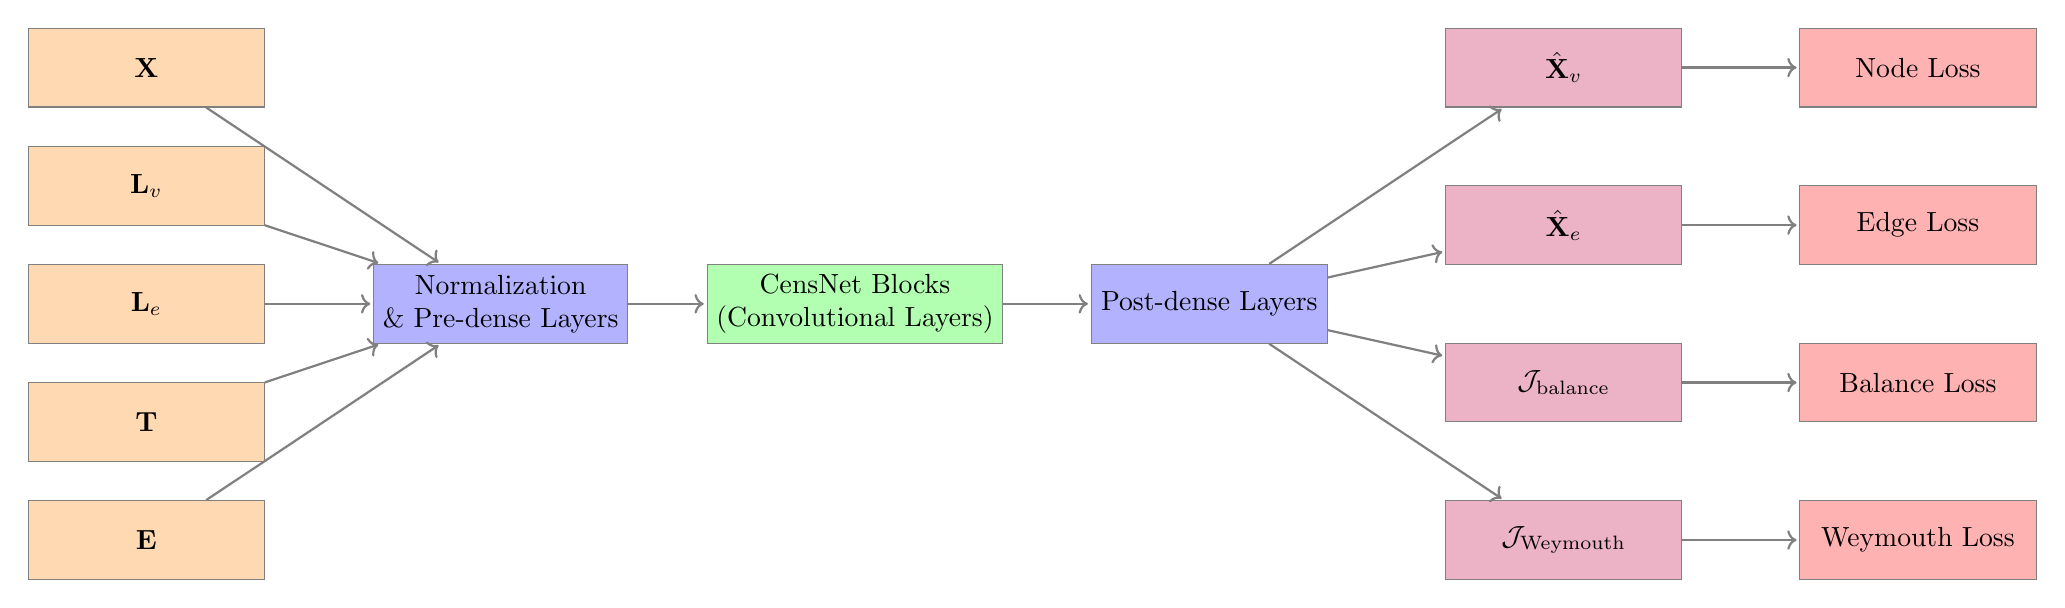
\begin{tikzpicture}[shorten >=1pt, ->, draw=black!50, node distance=1.5cm and 3.5cm, align=center]

    % Styles
    \tikzstyle{input} = [rectangle, draw, fill=orange!30, minimum width=3cm, minimum height=1cm]
    \tikzstyle{dense} = [rectangle, draw, fill=blue!30, minimum width=3cm, minimum height=1cm]
    \tikzstyle{conv} = [rectangle, draw, fill=green!30, minimum width=3cm, minimum height=1cm]
    \tikzstyle{output} = [rectangle, draw, fill=purple!30, minimum width=3cm, minimum height=1cm]
    \tikzstyle{loss} = [rectangle, draw, fill=red!30, minimum width=3cm, minimum height=1cm]
    \tikzstyle{arrow} = [->, thick]

    % Input Layer
    \node[input] (node_features) at (0,0) {\(\mathbf{X}\)};
    \node[input] (node_laplacian) [below of=node_features] {\(\mathbf{L}_v\)};
    \node[input] (edge_laplacian) [below of=node_laplacian] {\(\mathbf{L}_e\)};
    \node[input] (incidence_matrix) [below of=edge_laplacian] {\(\mathbf{T}\)};
    \node[input] (edge_features) [below of=incidence_matrix] {\(\mathbf{E}\)};

    % Normalization and Pre-dense Layer
    \node[dense] (norm_pre_dense) [right of=edge_laplacian, xshift=3cm] {Normalization \\ \& Pre-dense Layers};

    % Convolutional Layers
    \node[conv] (conv_layers) [right of=norm_pre_dense, xshift=3cm] {CensNet Blocks \\ (Convolutional Layers)};

    % Post-dense Layer
    \node[dense] (post_dense) [right of=conv_layers, xshift=3cm] {Post-dense Layers};

    % Outputs
    \node[output] (node_output) [right of=post_dense, xshift=3cm, yshift=3cm] {\(\hat{\mathbf{X}}_v\)};
    \node[output] (edge_output) [right of=post_dense, xshift=3cm, yshift=1cm] {\(\hat{\mathbf{X}}_e\)};
    \node[output] (balance_output) [right of=post_dense, xshift=3cm, yshift=-1cm] {\(\mathcal{J}_{\text{balance}}\)};
    \node[output] (weymouth_output) [right of=post_dense, xshift=3cm, yshift=-3cm] {\(\mathcal{J}_{\text{Weymouth}}\)};

    % Losses
    \node[loss] (node_loss) [right of=node_output, xshift=3cm] {Node Loss};
    \node[loss] (edge_loss) [right of=edge_output, xshift=3cm] {Edge Loss};
    \node[loss] (balance_loss) [right of=balance_output, xshift=3cm] {Balance Loss};
    \node[loss] (weymouth_loss) [right of=weymouth_output, xshift=3cm] {Weymouth Loss};

    % Arrows
    \draw[arrow] (node_features) -- (norm_pre_dense);
    \draw[arrow] (node_laplacian) -- (norm_pre_dense);
    \draw[arrow] (edge_laplacian) -- (norm_pre_dense);
    \draw[arrow] (incidence_matrix) -- (norm_pre_dense);
    \draw[arrow] (edge_features) -- (norm_pre_dense);

    \draw[arrow] (norm_pre_dense) -- (conv_layers);
    \draw[arrow] (conv_layers) -- (post_dense);

    \draw[arrow] (post_dense) -- (node_output);
    \draw[arrow] (post_dense) -- (edge_output);
    \draw[arrow] (post_dense) -- (balance_output);
    \draw[arrow] (post_dense) -- (weymouth_output);

    \draw[arrow] (node_output) -- (node_loss);
    \draw[arrow] (edge_output) -- (edge_loss);
    \draw[arrow] (balance_output) -- (balance_loss);
    \draw[arrow] (weymouth_output) -- (weymouth_loss);

\end{tikzpicture}

}

\vspace{0.8em}
Two additional loss terms were introduced to guide the training process using physical constraints from the gas balance and Weymouth equations.
\end{frame}



% \begin{frame}{Case Study I: 8-Node Network -- Performance Comparison}
% \scriptsize
% \centering
% \begin{table}
% \captionsetup{font=scriptsize}  % Cambia el tamaño del caption a \tiny
% \centering
% \begin{tabular}{lcccc}
% \toprule
% \textbf{Method} & \textbf{Node Error} & \textbf{Edge Error} & \textbf{Balance Error} & \textbf{Time (s)} \\
% \midrule
% CensNet (N) & $0.00 \pm 17.99$ & $22.76 \pm 15.43$ & $-0.01 \pm 17.45$ & $0.86 \pm 0.50$ \\
% CensNet (N+E) & $-0.11 \pm 18.27$ & $0.22 \pm 21.65$ & $-0.12 \pm 1.70$ & $0.85 \pm 0.50$ \\
% CensNet (N+E+B) & $-0.02 \pm 18.00$ & $-0.02 \pm 21.30$ & $-0.03 \pm 0.90$ & $0.85 \pm 0.50$ \\
% CensNet (N+E+W) & $-0.07 \pm 17.56$ & $2.60 \pm 20.03$ & $-0.07 \pm 2.21$ & $0.86 \pm 0.50$ \\
% CensNet (N+E+B+W) & $0.05 \pm 17.91$ & $0.25 \pm 21.14$ & $0.05 \pm 1.69$ & $0.85 \pm 0.50$ \\
% \bottomrule
% \end{tabular}
% % \caption{Performance of CensNet-based models vs. IPOPT benchmark.}
% \end{table}
%
% \begin{itemize}
%     \item Using only node loss leads to accurate nodal flows but large errors in edge predictions.
%     \item Adding edge loss (\textbf{N+E}) reduces edge error from $22.76$ to $0.22$ and improves global balance.
%     \item Including balance loss (\textbf{N+E+B}) further minimizes balance error, achieving best overall consistency.
%     \item Weymouth loss (\textbf{N+E+W}) introduces slight trade-offs, slightly increasing edge/balance errors but retaining nodal accuracy.
%     \item All CensNet variants are over an order of magnitude faster than IPOPT, with \textbf{N+E+B} offering the best accuracy-speed compromise.
% \end{itemize}
%
% \end{frame}


\begin{frame}{Case Study I: 8-Node Network -- Performance Comparison}
\scriptsize
\begin{table}
\captionsetup{font=scriptsize}  % Cambia el tamaño del caption a \tiny
\hfill  % Empuja la tabla a la derecha
\begin{tabular}{lcccc}
\toprule
\textbf{Method} & \textbf{Node Error} & \textbf{Edge Error} & \textbf{Balance Error} & \textbf{Time (s)} \\
\midrule
CensNet (N) & $0.00 \pm 17.99$ & $22.76 \pm 15.43$ & $-0.01 \pm 17.45$ & $0.86 \pm 0.50$ \\
CensNet (N+E) & $-0.11 \pm 18.27$ & $0.22 \pm 21.65$ & $-0.12 \pm 1.70$ & $0.85 \pm 0.50$ \\
CensNet (N+E+B) & $-0.02 \pm 18.00$ & $-0.02 \pm 21.30$ & $-0.03 \pm 0.90$ & $0.85 \pm 0.50$ \\
CensNet (N+E+W) & $-0.07 \pm 17.56$ & $2.60 \pm 20.03$ & $-0.07 \pm 2.21$ & $0.86 \pm 0.50$ \\
CensNet (N+E+B+W) & $0.05 \pm 17.91$ & $0.25 \pm 21.14$ & $0.05 \pm 1.69$ & $0.85 \pm 0.50$ \\
\bottomrule
\end{tabular}
\end{table}

\begin{itemize}
    \item Using only node loss leads to accurate nodal flows but large errors in edge predictions.
    \item Adding edge loss (\textbf{N+E}) reduces edge error from $22.76$ to $0.22$ and improves global balance.
    \item Including balance loss (\textbf{N+E+B}) further minimizes balance error, achieving best overall consistency.
    \item Weymouth loss (\textbf{N+E+W}) introduces slight trade-offs, slightly increasing edge/balance errors but retaining nodal accuracy.
    \item All CensNet variants are over an order of magnitude faster than IPOPT, with \textbf{N+E+B} offering the best accuracy-speed compromise.
\end{itemize}

\end{frame}


% % % --- Slide 2: Main Observations ---
% \begin{frame}{Case Study I: Key Observations}
% \begin{itemize}
%     \item Using only node loss leads to accurate nodal flows but large errors in edge predictions.
%     \item Adding edge loss (\textbf{N+E}) reduces edge error from $22.76$ to $0.22$ and improves global balance.
%     \item Including balance loss (\textbf{N+E+B}) further minimizes balance error, achieving best overall consistency.
%     \item Weymouth loss (\textbf{N+E+W}) introduces slight trade-offs, slightly increasing edge/balance errors but retaining nodal accuracy.
%     \item All CensNet variants are over an order of magnitude faster than IPOPT, with \textbf{N+E+B} offering the best accuracy-speed compromise.
% \end{itemize}
% \end{frame}


% \begin{frame}{Stochastic Analysis: Methodology and results}
% \footnotesize
%     \textbf{Methodology:}
%     \begin{itemize}
%         \item Kernel Density Estimate (KDE) fitted to training inputs.
%         \item Synthetic samples generated and propagated through CensNet.
%         \item Log-likelihoods compared for $y_{\text{sample}}$ and $\bar{y}_{\text{train}}$.
%         \item Kolmogorov–Smirnov (K–S) test used for distributional similarity.
%     \end{itemize}
%
%     \vspace{0.5em}
%     \textbf{Results:}
%     \begin{itemize}
%         \item Log-likelihoods: $y_{\text{sample}} = -6.696 \times 10^6$, 
%               $\bar{y}_{\text{train}} = -6.657 \times 10^6$.
%         \item K–S test: $p > 0.44$ across all alternatives.
%         \item $\Rightarrow$ Synthetic outputs statistically consistent with training outputs.
%     \end{itemize}
%
% \end{frame}

% \begin{frame}{Model Robustness under Uncertainty}
%     \begin{itemize}
%         \item Log-likelihoods: $y_{\text{sample}} = -6.696 \times 10^6$, 
%               $\bar{y}_{\text{train}} = -6.657 \times 10^6$.
%         \item K–S test: $p > 0.44$ across all alternatives.
%         \item $\Rightarrow$ Synthetic outputs statistically consistent with training outputs.
%     \end{itemize}
% \end{frame}

\begin{frame}{Negative Flows in Pipeline $p_3$}
\scriptsize
    \begin{itemize}
        \item Flow in $p_3$ consistently negative across scenarios and KDE samples.
        \item Caused by orientation assumption $\rightarrow$ optimizer adjusts direction.
        \item Operability unaffected, but $p_3$ supports cost minimization.
    \end{itemize}
    \begin{figure}
        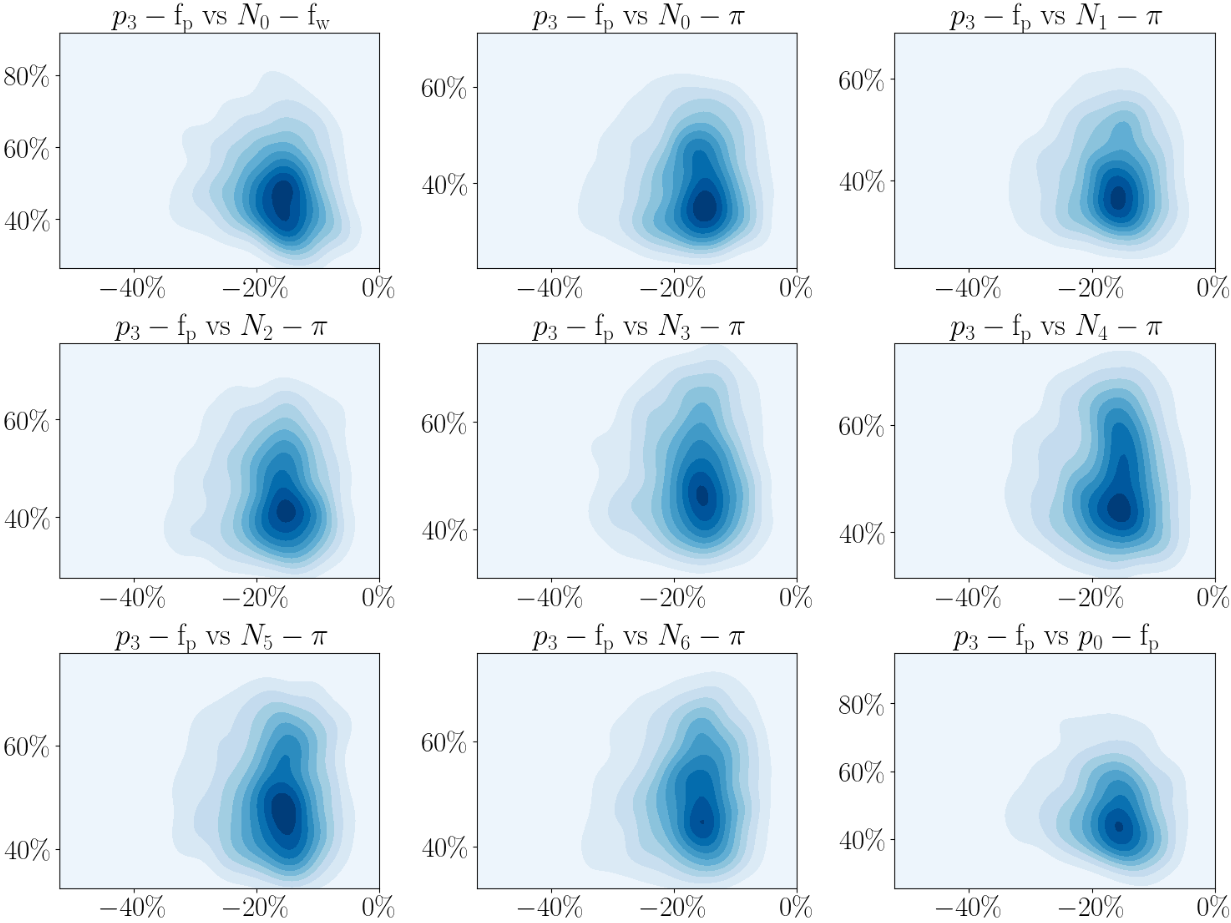
\includegraphics[width=0.65\textwidth]{figures/outputs_outputs_2_cut.png}
        % \caption{\scriptsize Joint PDFs showing negative $p_3$ flows.}
    \end{figure}
\end{frame}

\begin{frame}{Pressure Concentration in Mid-Range}
\scriptsize
% por revisar
    \begin{itemize}
        \item Nodal pressures cluster at 30--40\% of normalized limits.
        \item Avoids extremes, ensuring reliable operation.
        \item Implies optimizer favors efficiency + stability.
    \end{itemize}
    \begin{figure}
        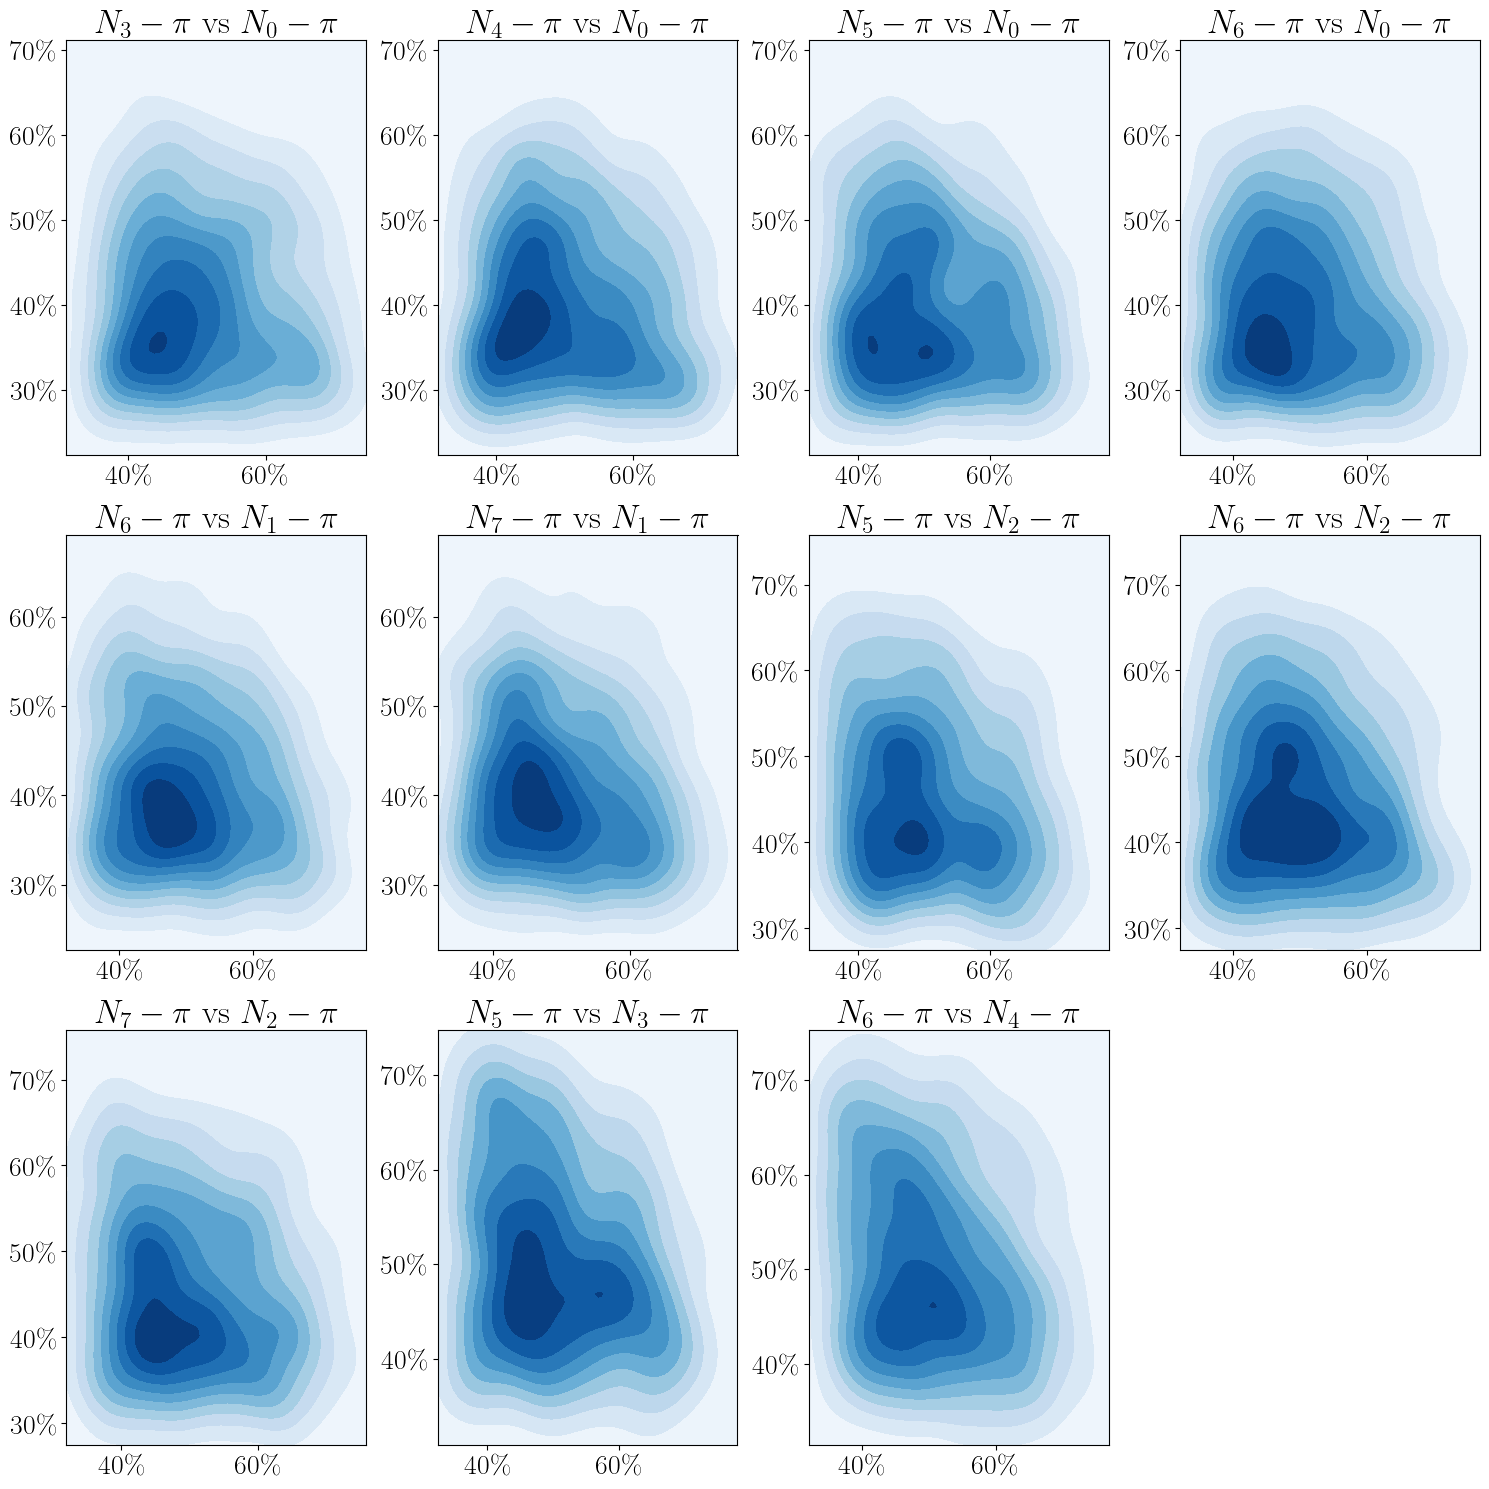
\includegraphics[width=0.5\textwidth]{figures/outputs_outputs_3.png}
        % \caption{\scriptsize Pressures concentrate in mid-range (30--40\%).}
    \end{figure}
\end{frame}


\begin{frame}{Stable Utilization of Pipeline $p_4$}
\scriptsize
% revisar
    \begin{itemize}
        \item Despite wide dispersion in inputs, $p_4$ flow remains 20--40\%.
        \item Reflects robustness: optimizer stabilizes this delivery path.
        \item Behavior consistently learned and reproduced in KDE samples.
    \end{itemize}
    \begin{figure}
        \includegraphics[width=0.7\textwidth]{figures/inputs_outputs_1.png}
        % \caption{\scriptsize Optimization model: input variability vs. stable $p_4$ flow.}
    \end{figure}
    % \begin{figure}
    %     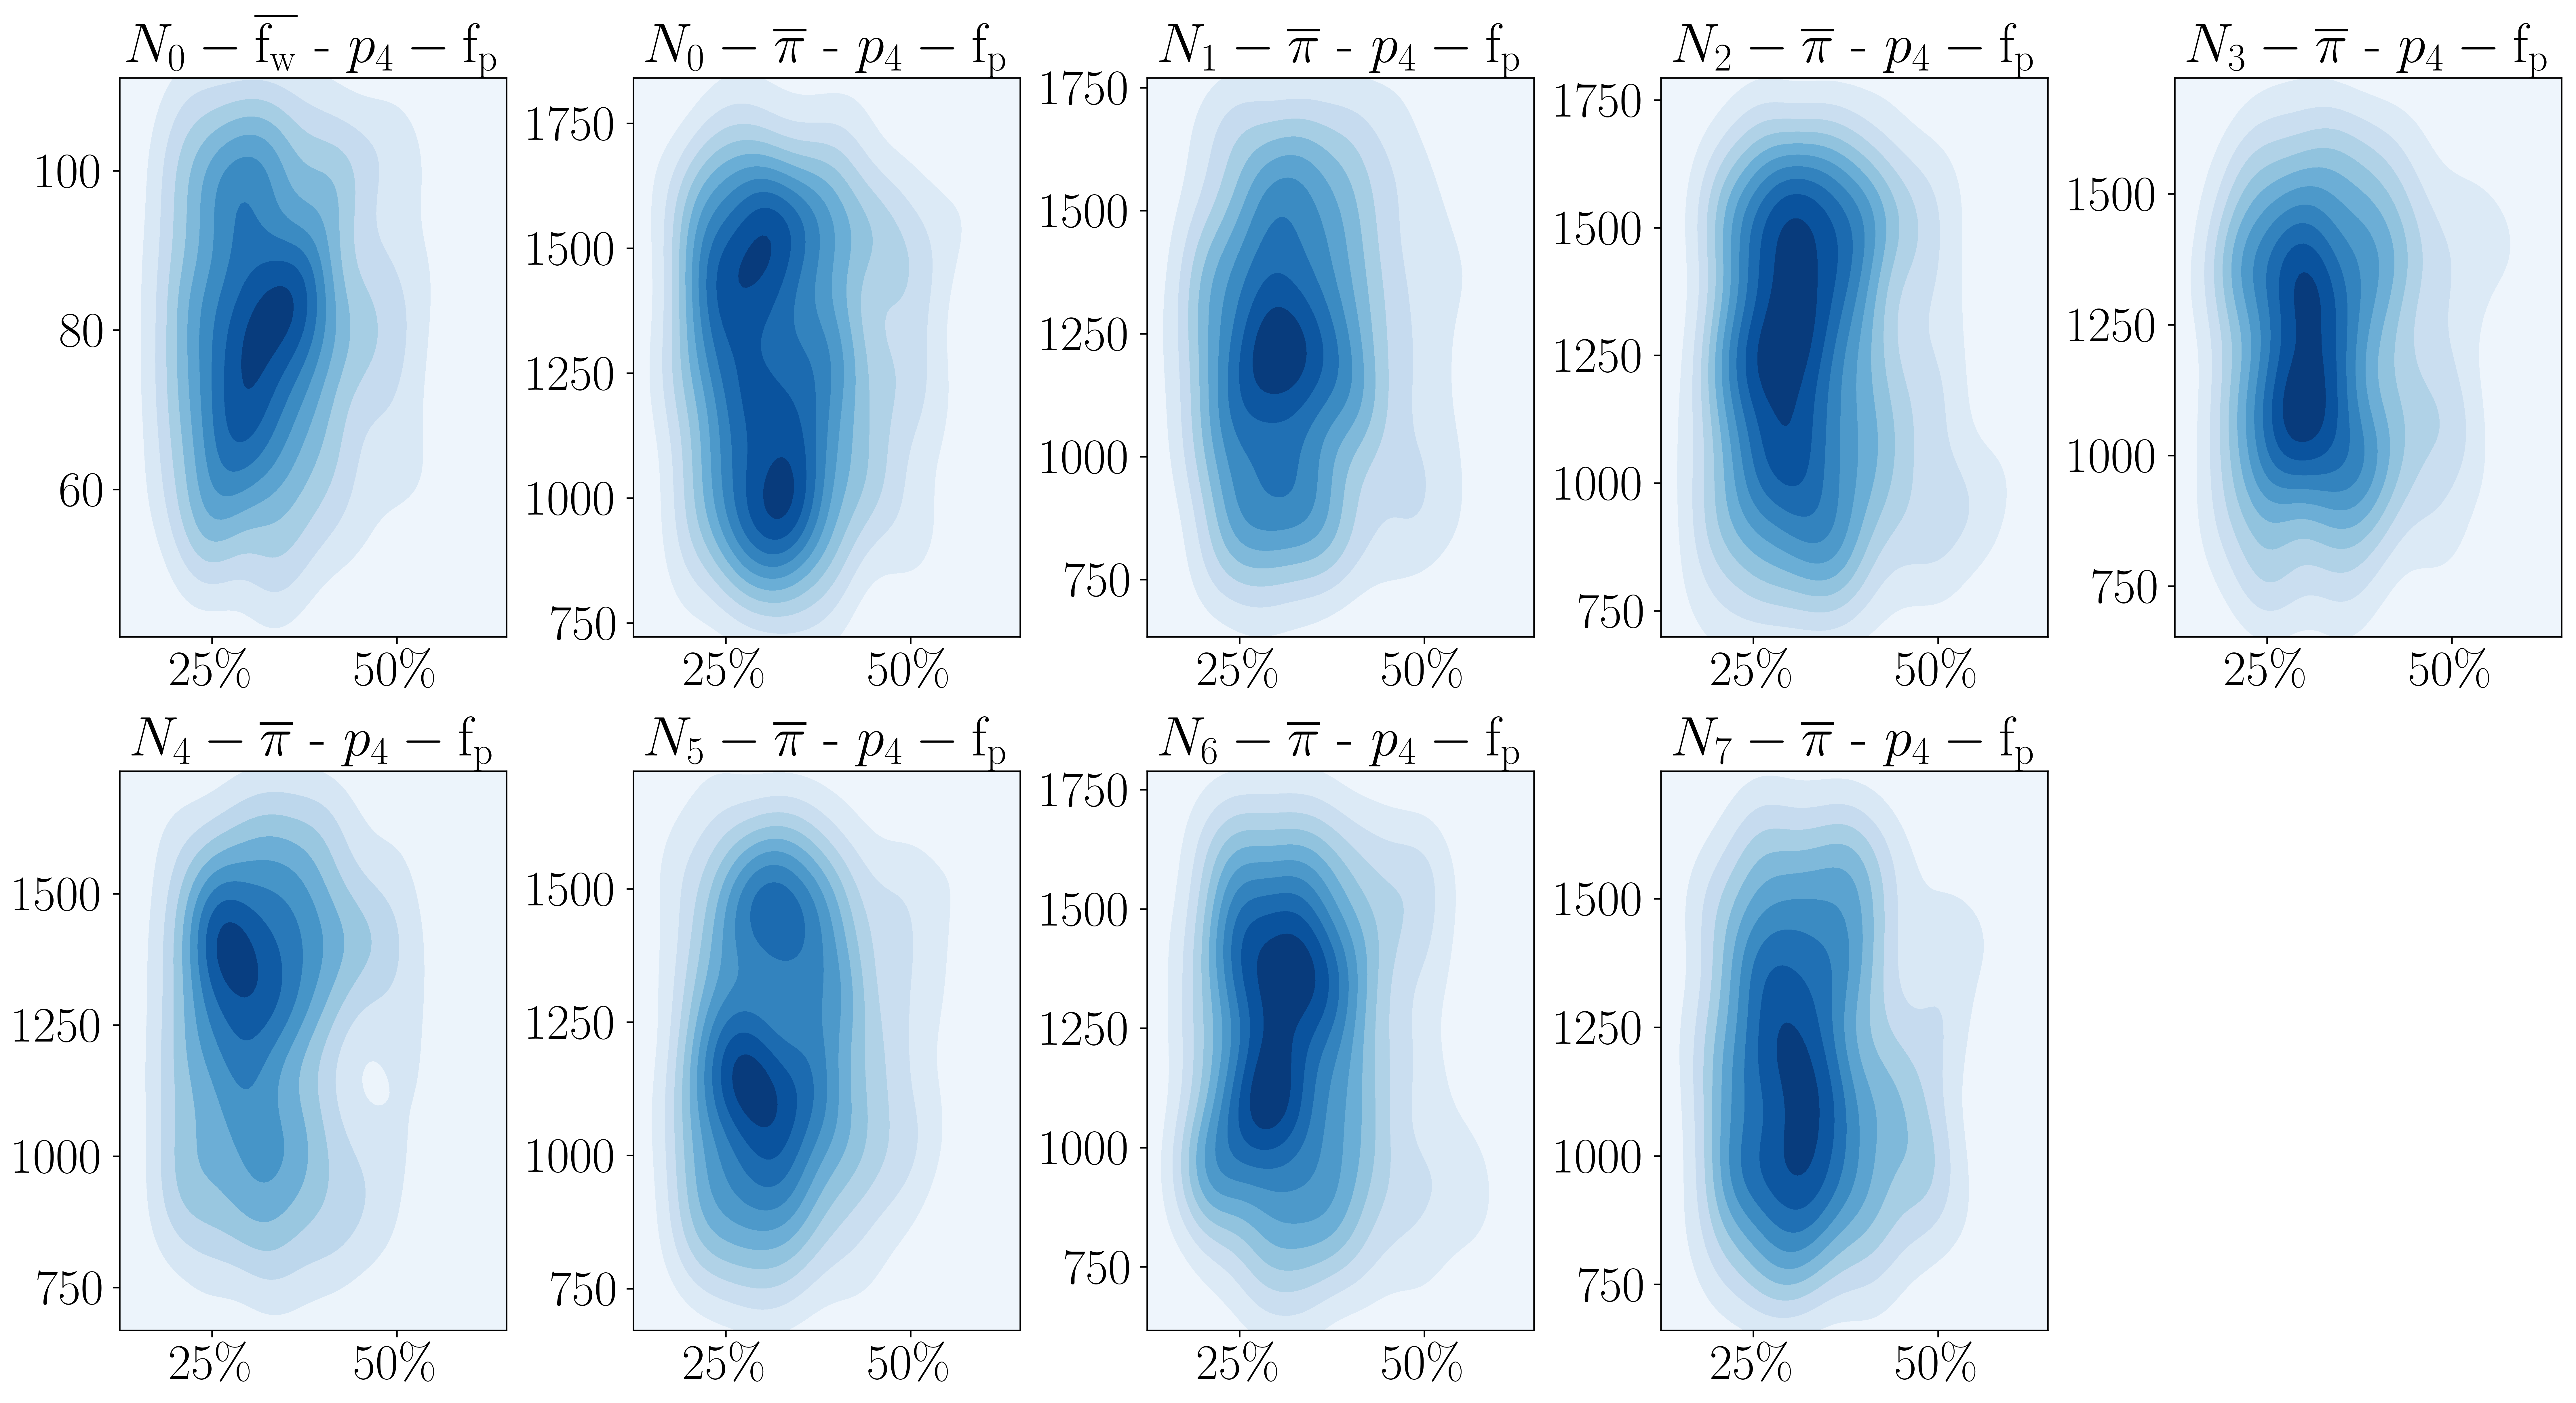
\includegraphics[width=0.7\textwidth]{figures/Chapter_NonLinealCensnet/inputs_outputs_1_KDE.png}
    %     \caption*{KDE samples confirm concentration of $p_4$ flow at 20--40\%.}
    % \end{figure}
\end{frame}

\begin{frame}{Linear Input--Output Relations}
\scriptsize
% Por revisar
    \begin{itemize}
        \item Positive correlation: demand bounds ($N_6$, $N_7$) vs. $p_4$--$p_7$ flows.
        \item Negative correlation: $N_7$ demand bound vs. $p_3$ flow.
        \item Shows network internalized optimizer’s allocation strategies.
    \end{itemize}
    \begin{figure}
        \includegraphics[width=0.5\textwidth]{figures/inputs_outputs_2.png}
        % \caption{\scriptsize Optimization model: linear input–output patterns.}
    \end{figure}
    % \begin{figure}
    %     \includegraphics[width=0.7\textwidth]{figures/Chapter_NonLinealCensnet/inputs_outputs_2_KDE.png}
    %     \caption*{KDE samples replicate both positive and negative correlations.}
    % \end{figure}
    \textbf{Results:}
    \begin{itemize}
        \item Log-likelihoods: $y_{\text{sample}} = -6.696 \times 10^6$, 
              $\bar{y}_{\text{train}} = -6.657 \times 10^6$.
        \item K–S test: $p > 0.44$ across all alternatives.
        \item $\Rightarrow$ Synthetic outputs statistically consistent with training outputs.
    \end{itemize}
%

\end{frame}

\section{Conclusions and Future Work}
\begin{frame}{Conclusions}
    \begin{itemize}
        \item \textbf{GNN-based prediction:} CensNet achieved accurate and scalable predictions for natural gas networks, with significant reductions in computation time compared to traditional optimization.
        \item \textbf{Optimization with MPCC:} Proposes a formulation to approximate Weymouth's restrictions, improving accuracy of pressure–flow representation and showing robustness in real-world scheduling tasks.
        \item \textbf{Stochastic modeling:} Physics-guided neural networks preserved structural dependencies and generalized reliably under uncertainty, validated through KDE sampling and K–S testing.
        \item \textbf{Overall:} Integrating physical constraints with GNNs yields efficient, accurate, and robust surrogates for optimization in natural gas systems.
    \end{itemize}
\end{frame}

% \begin{frame}{Future Work}
%     \begin{itemize}
%         \item Extend stochastic framework toward \textbf{full stochastic optimization} for gas–power coordination.
%         \item Explore \textbf{physics-informed neural operators} to improve learning of nonlinear constraints (e.g., Weymouth).
%         \item Incorporate \textbf{real operational data} from SCADA systems to validate scalability in live environments.
%         \item Investigate \textbf{transfer learning across networks}, enabling models trained on one topology to adapt to others with minimal retraining.
%         \item Apply developed methods to \textbf{decision-support tools} for dispatchers in interconnected energy systems.
%     \end{itemize}
% \end{frame}


\begin{frame}{Future Work}
\begin{itemize}
    \item Extend GNN-based models to capture \textbf{transient dynamics} and \textbf{operational uncertainty}.
    \item Develop \textbf{stochastic MPCC formulations} to handle variability from renewables and uncertain demand.
    % \item Design \textbf{physics-guided loss functions} (e.g., Weymouth) that balance accuracy and computational efficiency.
    % \item Test scalability and robustness using \textbf{real operational data}.
    \item Integrate with \textbf{climatological forecasting tools} to anticipate gas consumption and interactions with renewable energy sources.
\end{itemize}
\end{frame}



\begin{frame}{Products}
\footnotesize
\textbf{Publications}
\begin{itemize}
    \item \textbf{Paper A1:} \emph{Optimization of Interconnected Natural Gas and Power Systems Using Mathematical Programs with Complementarity Constraints}.\\
    Journal: \textit{Mathematics}.\\
    DOI: \href{https://doi.org/10.3390/math12142224}{10.3390/math12142224}.
    
    \item \textbf{Proceedings:} \emph{Approximation of Weymouth Equation Using Mathematical Programs with Complementarity Constraints for Natural Gas Transportation}.\\
    Journal: \textit{Engineering Proceedings}.\\
    DOI: \href{https://doi.org/10.3390/engproc2023039091}{10.3390/engproc2023039091}.
\end{itemize}

\vspace{0.6em}

\textbf{Software}
\begin{itemize}
    \item \emph{OPTIGASFLOW: Optimizando el Flujo de Gas Natural}.\\
    Libro - Tomo - Partida: 13-97-23. \\
    Registro: 01-dic.-2023.
\end{itemize}
\end{frame}



\begin{frame}{Acknowledgments}
    \begin{itemize}
        \item Gratitude to the Maestría en Ingenieríaa Eléctrica, graduate program of the Universidad Tecnológica de Pereira, for their support in the project E6-24-1.
        \item Special thanks to the Minciencias project: “Desarrollo de una herramienta para la planeación a largo plazo de la operación del sistema de transporte de gas natural de Colombia”—código de registro 69982—part of the ”CONVOCATORIA DE PROYECTOS CONECTANDO CONOCIMIENTO 2019 852-2019”.
        \item Acknowledgment to the Automatics Research Group of the Universidad Tecnológica de Pereira for their invaluable support in the development of the project outcomes.
    \end{itemize}

    \vfill % pushes logos to the bottom
    \begin{center}
        
\includegraphics[height=1.5cm]{figures/logos/minciencias_logo.png}
        
\includegraphics[height=1.5cm]{figures/logos/mie.jpg} 
        
\includegraphics[height=1.5cm]{figures/logos/automatica.jpeg}
    \end{center}
\end{frame}


% \section{Bibliography}
\begin{frame}[allowframebreaks]
        \frametitle{References}
        \bibliographystyle{apalike}
        \bibliography{biblio}
\end{frame}



\end{document}
